\documentclass[12pt]{report}
\usepackage[spanish]{babel}
\usepackage[a4paper, margin=1in]{geometry}
\usepackage{graphicx}
\graphicspath{{images/}}
\usepackage{times}
\usepackage{setspace}
\linespread{1.5}
\usepackage{tabularx}
\usepackage[colorlinks=true, linkcolor=black, citecolor=black, urlcolor=black]{hyperref}
\usepackage{apacite}
\bibliographystyle{apacite}
\setlength\extrarowheight{2pt}
\usepackage{longtable}
\usepackage{ltablex}
\usepackage{booktabs}
\usepackage{titlesec}
\usepackage{amsmath, amssymb}

\titlespacing{\chapter}{0pt}{0pt}{40pt}

% Formato para evitar la separación de palabras 
\tolerance=1
\emergencystretch=\maxdimen
\hyphenpenalty=10000
\hbadness=10000

% Formato de números de páginas
\usepackage{fancyhdr}
\fancyhf{}
\setlength{\headheight}{15pt}

\fancypagestyle{plain}{
    \fancyhf{}
    \fancyfoot[C]{\thepage}
    \renewcommand{\headrulewidth}{0pt}
    \renewcommand{\footrulewidth}{0pt}
}

\renewcommand{\headrulewidth}{0pt}
\renewcommand{\thechapter}{\Roman{chapter}}

% Formato de sangrías y listas
\usepackage{enumitem}
\renewcommand{\labelitemi}{$\bullet$}
\setlength{\parindent}{0.4in}
\setlist[itemize,1]{leftmargin=0.35in}
\setlist[itemize]{leftmargin=0.2in}

% Formato de la tabla de contenido
\usepackage{tocloft}
\addto\captionsspanish{
  \renewcommand{\contentsname}{Índice de Contenido}
  \renewcommand{\listfigurename}{Índice de Figuras}
  \renewcommand{\listtablename}{Índice de Tablas}
}
\renewcommand{\cfttoctitlefont}{\hfill\normalsize\bfseries}
\renewcommand{\cftaftertoctitle}{\hfill}
\renewcommand{\cftloftitlefont}{\hfill\normalsize\bfseries}
\renewcommand{\cftafterloftitle}{\hfill}
\renewcommand{\cftlottitlefont}{\hfill\normalsize\bfseries}
\renewcommand{\cftafterlottitle}{\hfill}
\setlength{\cftbeforetoctitleskip}{-20pt}
\setlength{\cftbeforeloftitleskip}{-20pt}
\setlength{\cftbeforelottitleskip}{-20pt}
\setcounter{secnumdepth}{4}
\setcounter{tocdepth}{4}


% TOC Chapter Style
\setlength{\cftbeforechapskip}{5pt}
\renewcommand{\cftchapdotsep}{\cftdotsep}

% TOC Sections Style
\setlength{\cftsecindent}{0pt}
\setlength{\cftsubsecindent}{1.5em}
\setlength{\cftsubsubsecindent}{3em}
\setlength{\cftparaindent}{4.5em}

% Formato de los diferentes niveles de secciones
\newcommand{\upper}[1]{\uppercase{#1}}
\usepackage{titlesec}
\titleformat{\chapter}
{\normalfont\fontsize{12}{15}\bfseries\centering}{}{0.3em}{}[\thispagestyle{empty}]
\titleformat{\section}
{\normalfont\fontsize{12}{15}\bfseries}{\thesection}{1em}{}
\titleformat{\subsection}
{\normalfont\fontsize{12}{15}\bfseries\narrower}{\thesubsection}{1em}{}
\titleformat{\subsubsection}
{\normalfont\fontsize{12}{15}\bfseries\itshape\narrower}{\thesubsubsection}{1em}{}
\titleformat{\paragraph}
{\normalfont\fontsize{12}{15}\itshape\narrower}{\theparagraph}{1em}{}

% Comandos para crear secciones no numeradas con entrada en el índice
\newcommand{\uchapter}[1]{
  \addtocounter{chapter}{1}
  \phantomsection
  \chapter*{Capítulo \thechapter. {#1}}
  \addcontentsline{toc}{chapter}{Capítulo \thechapter. {#1}}
}
\newcommand{\uextra}[2]{
  \addtocounter{chapter}{1}
  \phantomsection
  \chapter*{{#1} \thechapter. {#2}}
  \addcontentsline{toc}{chapter}{{#1} \thechapter. {#2}}
}
\newcommand{\usection}[1]{
  \phantomsection
  \section*{#1}
  \addcontentsline{toc}{section}{#1}
}
\newcommand{\usubsection}[1]{
  \phantomsection
  \subsection*{#1.}
  \addcontentsline{toc}{subsection}{#1}
}
\newcommand{\usubsubsection}[1]{
  \phantomsection
  \subsubsection*{#1.}
  \addcontentsline{toc}{subsubsection}{#1}
}
\newcommand{\uparagraph}[1]{
  \phantomsection
  \paragraph*{#1.}
  \addcontentsline{toc}{paragraph}{#1}
}

\newcommand{\listequationsname}{Índice de Ecuaciones}
\newlistof{myequations}{equ}{\listequationsname}
\newcommand{\myequations}[1]{
  \addcontentsline{equ}{myequations}{\protect\numberline{\theequation} #1}\par
}

\makeatletter
\renewcommand{\listofmyequations}{%
  \section*{\hfill\normalsize\bfseries Índice de Fórmulas\hfill}%
  \vspace{-20pt}
  \vspace{4em}
  \@starttoc{equ}
}
\makeatother

\usepackage{calc}
\renewcommand{\cftfigpresnum}{Figura~}
\setlength{\cftfignumwidth}{\widthof{Figura IV.1 }}

\renewcommand{\cfttabpresnum}{Tabla~}
\setlength{\cfttabnumwidth}{\widthof{Tabla IV.1 }}

\renewcommand{\cftmyequationspresnum}{Fórmula }
\setlength{\cftmyequationsindent}{1.5em}
\setlength{\cftmyequationsnumwidth}{\widthof{Fórmula IV.1 }}

\begin{document}

\pagenumbering{gobble}
\titleformat{\chapter}
{\normalfont\fontsize{12}{15}\centering}{Anexos \thechapter.}{0.3em}{}[]

\clearpage
\thispagestyle{empty}
\begin{center}
  \vspace*{\fill}
  \phantomsection
  Apéndices
  \addcontentsline{toc}{chapter}{Anexos}
  \vspace*{\fill}
\end{center}
\clearpage

\appendix
% \uextra{Apendice}{Dispositivo Raspberry Pi 4 Model B}
% \begin{figure}[ht!]
%   \centering
%   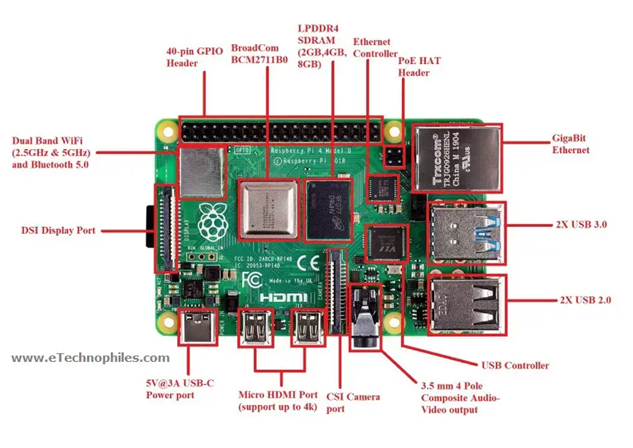
\includegraphics[width=0.95\textwidth]{Anexos/1.arquitectura-raspberry.png}
%   \caption{Arquitectura del Raspberry Pi 4 Model B}
%   \label{fig:raspberry-architecture}
% \end{figure}

\uextra{Apendice}{Representación cíclica del tiempo mediante funciones trigonométricas}
\begin{figure}[ht!]
  \centering
  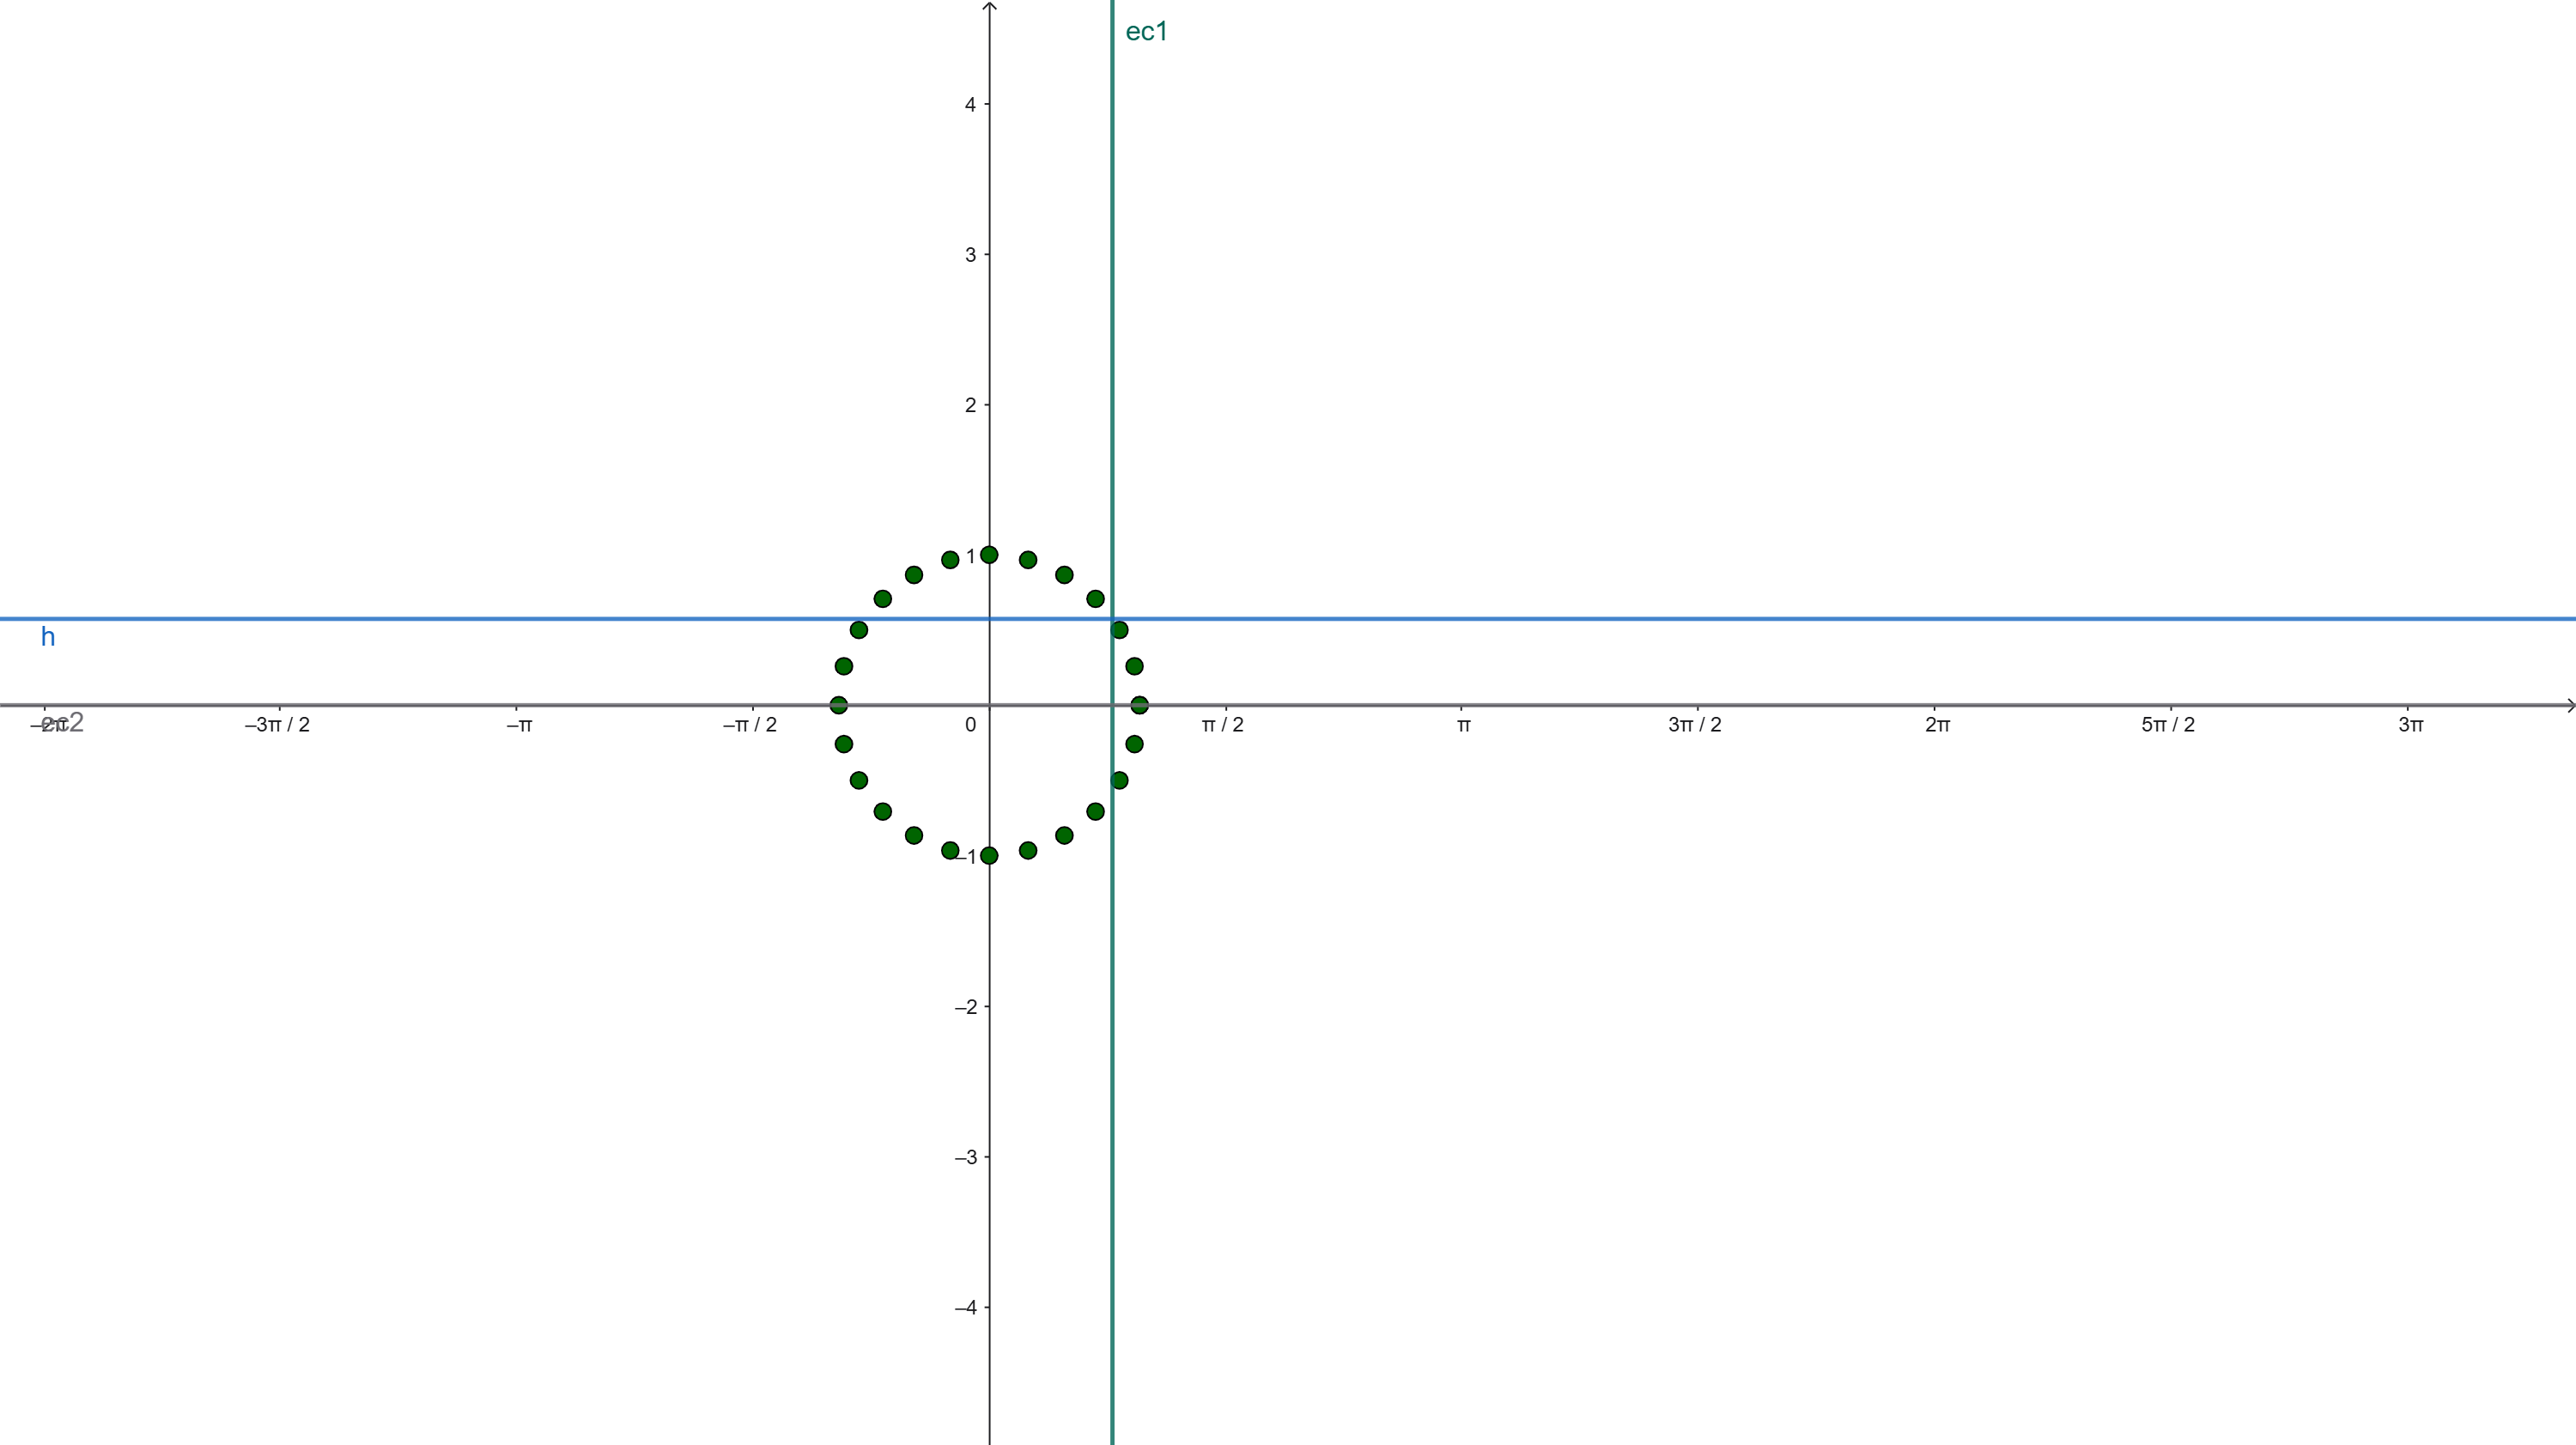
\includegraphics[width=0.55\textwidth]{Apendices/rc.png}
  \caption{Visualización discreta del comportamiento cíclico del tiempo} 
  \caption*{GeoGebra: Generación de puntos discretos sobre la circunferencia usando la expresión: \newline
  \texttt{Sequence((cos(2$\pi$ * n / 86400), sin(2$\pi$ * n / 86400)), n, 0, 86400, 3600)}}
  \caption*{La figura incluye dos líneas auxiliares que recorren la circunferencia: una horizontal (coseno) y una vertical (seno), generadas dinámicamente mediante un deslizador \( t \) con paso de 600 segundos. Estas líneas intersectan en el punto \( (x, y) \), representando la posición temporal proyectada en coordenadas trigonométricas.}
  \label{fig:representacion-ciclica-tiempo}
\end{figure}

\begin{figure}[ht!]
  \centering
  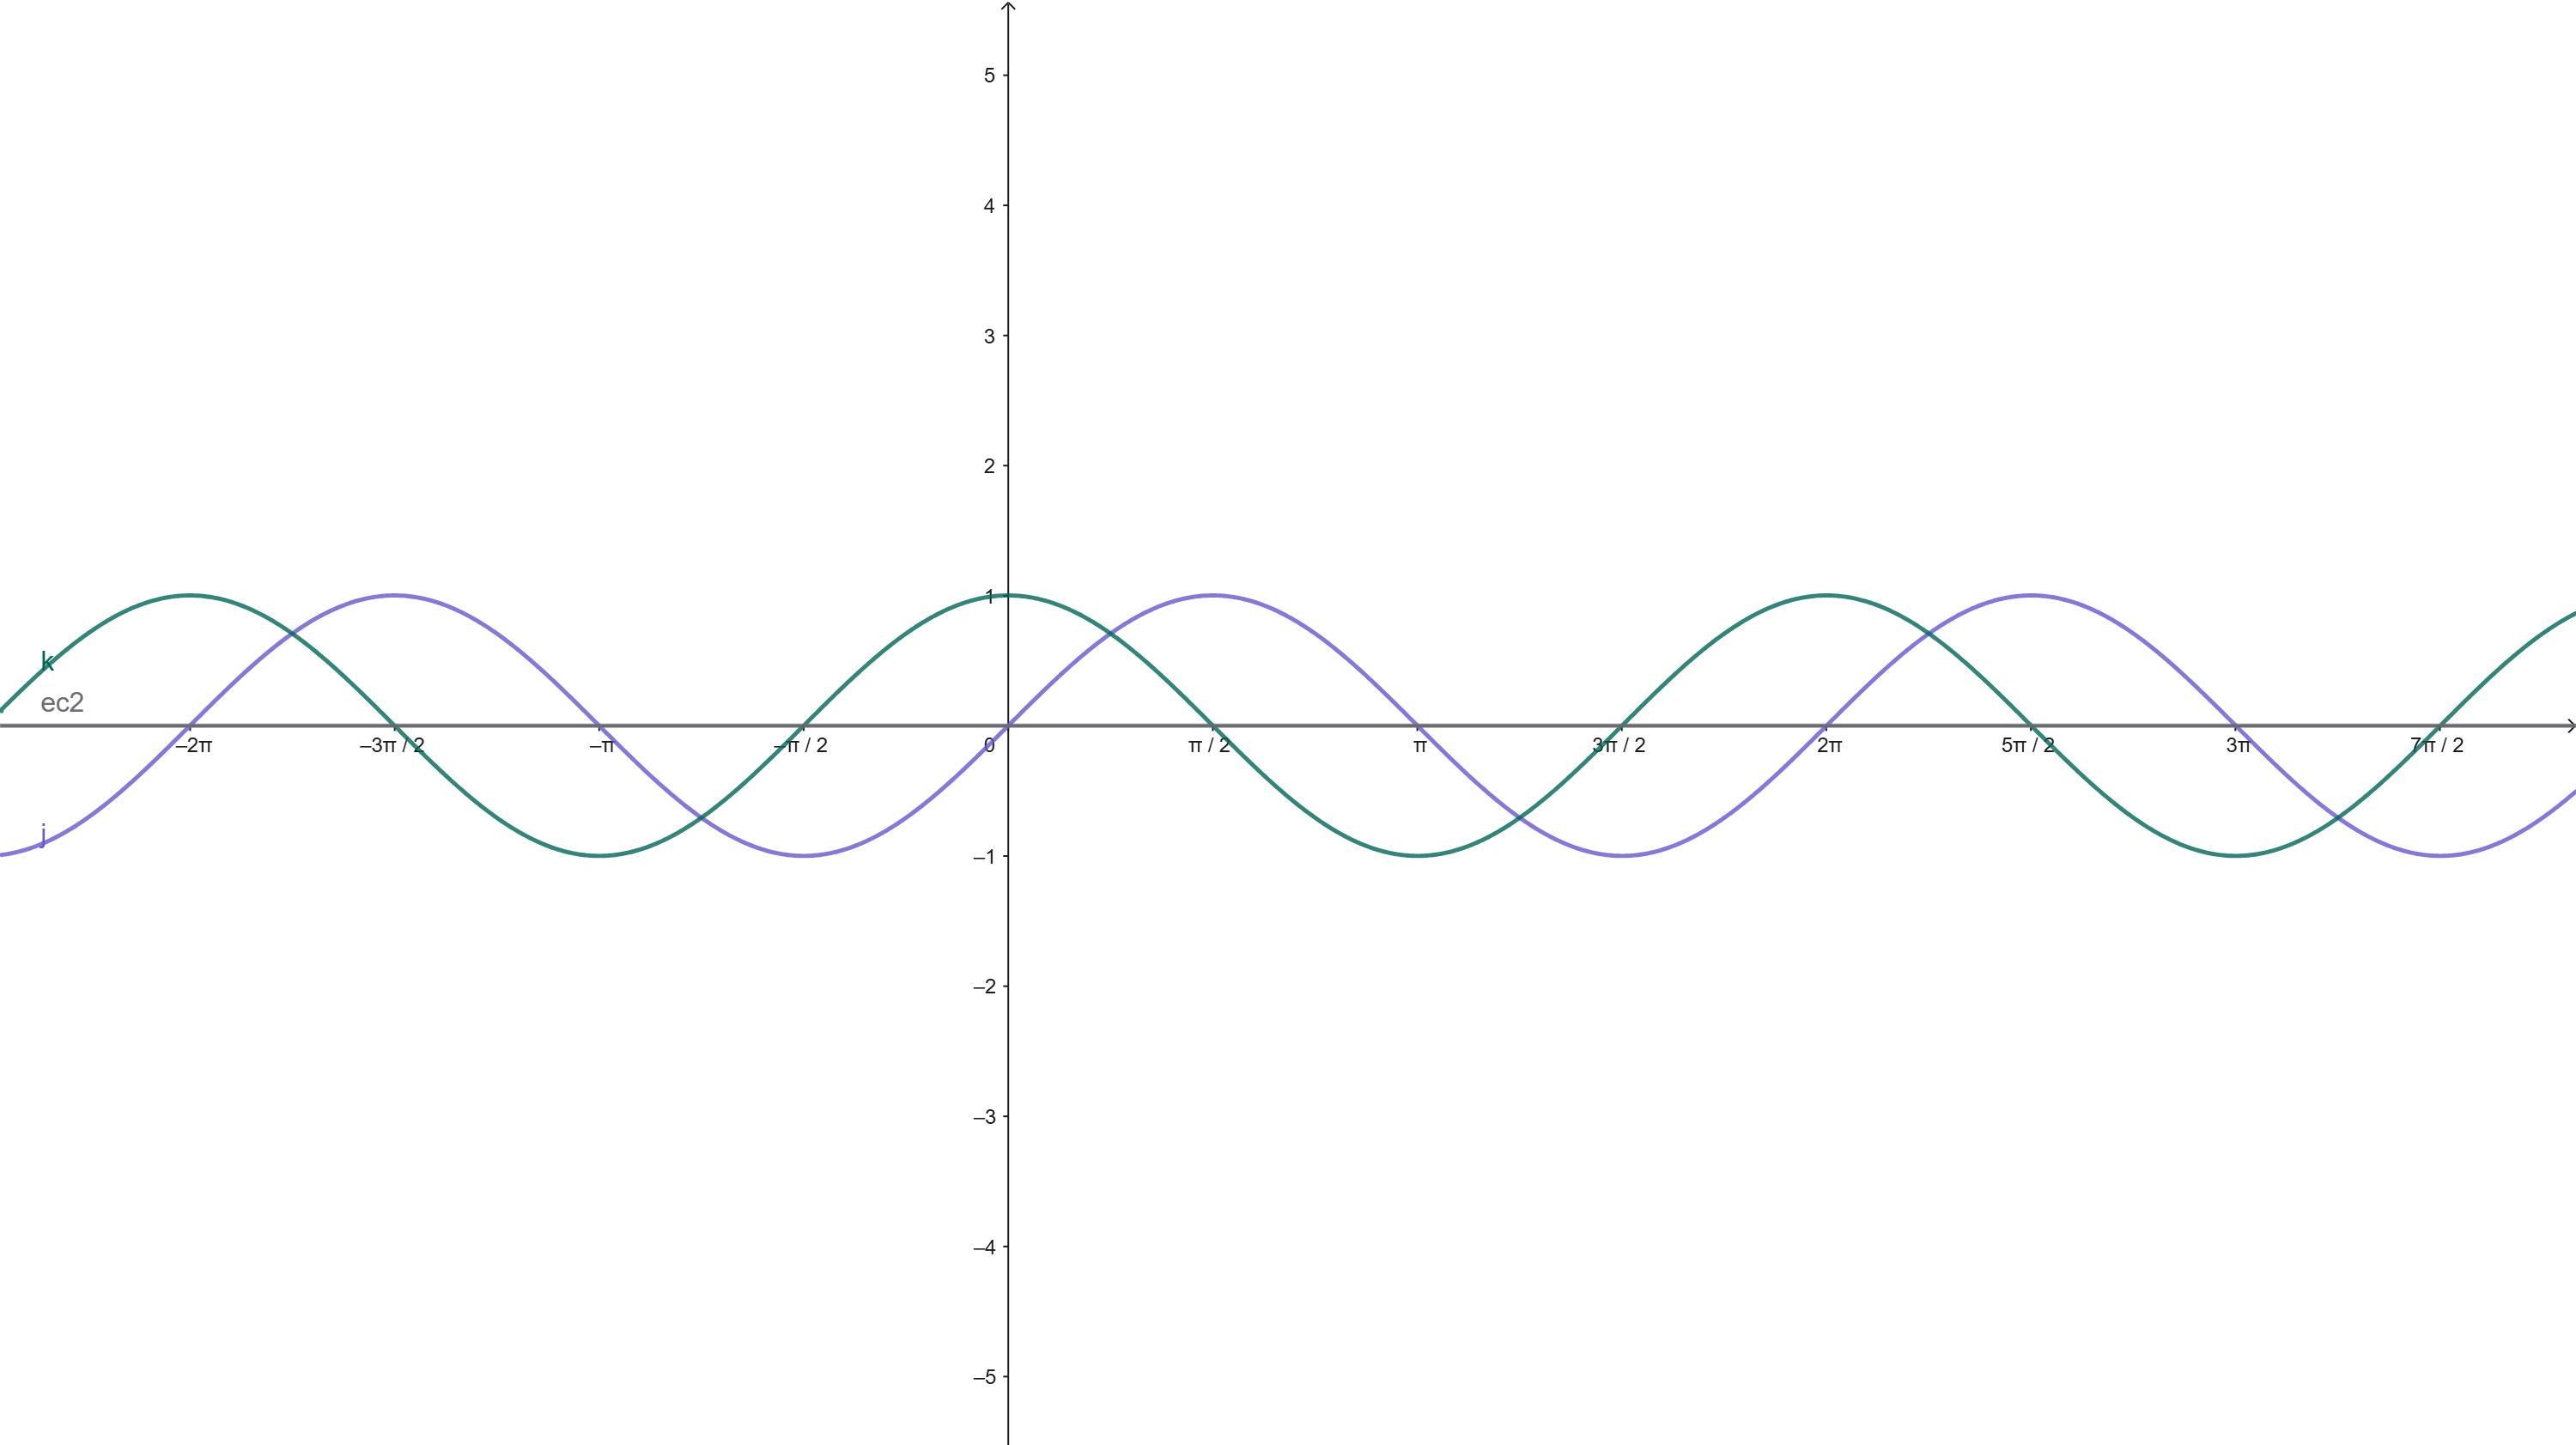
\includegraphics[width=0.55\textwidth]{Apendices/sencos.png}
  \caption{Visualización de las funciones seno y coseno  } 
  \caption*{GeoGebra: Generación de las funciones seno y coseno usando las expresiones: \newline
  \texttt{Sequence((x, sin(x)), x, 0, 2$\pi$, $\pi$/6)} y \newline
  \texttt{Sequence((x, cos(x)), x, 0, 2$\pi$, $\pi$/6)}}
  \label{fig: seno-coseno}
\end{figure}

\begin{figure}[ht!]
  \centering
  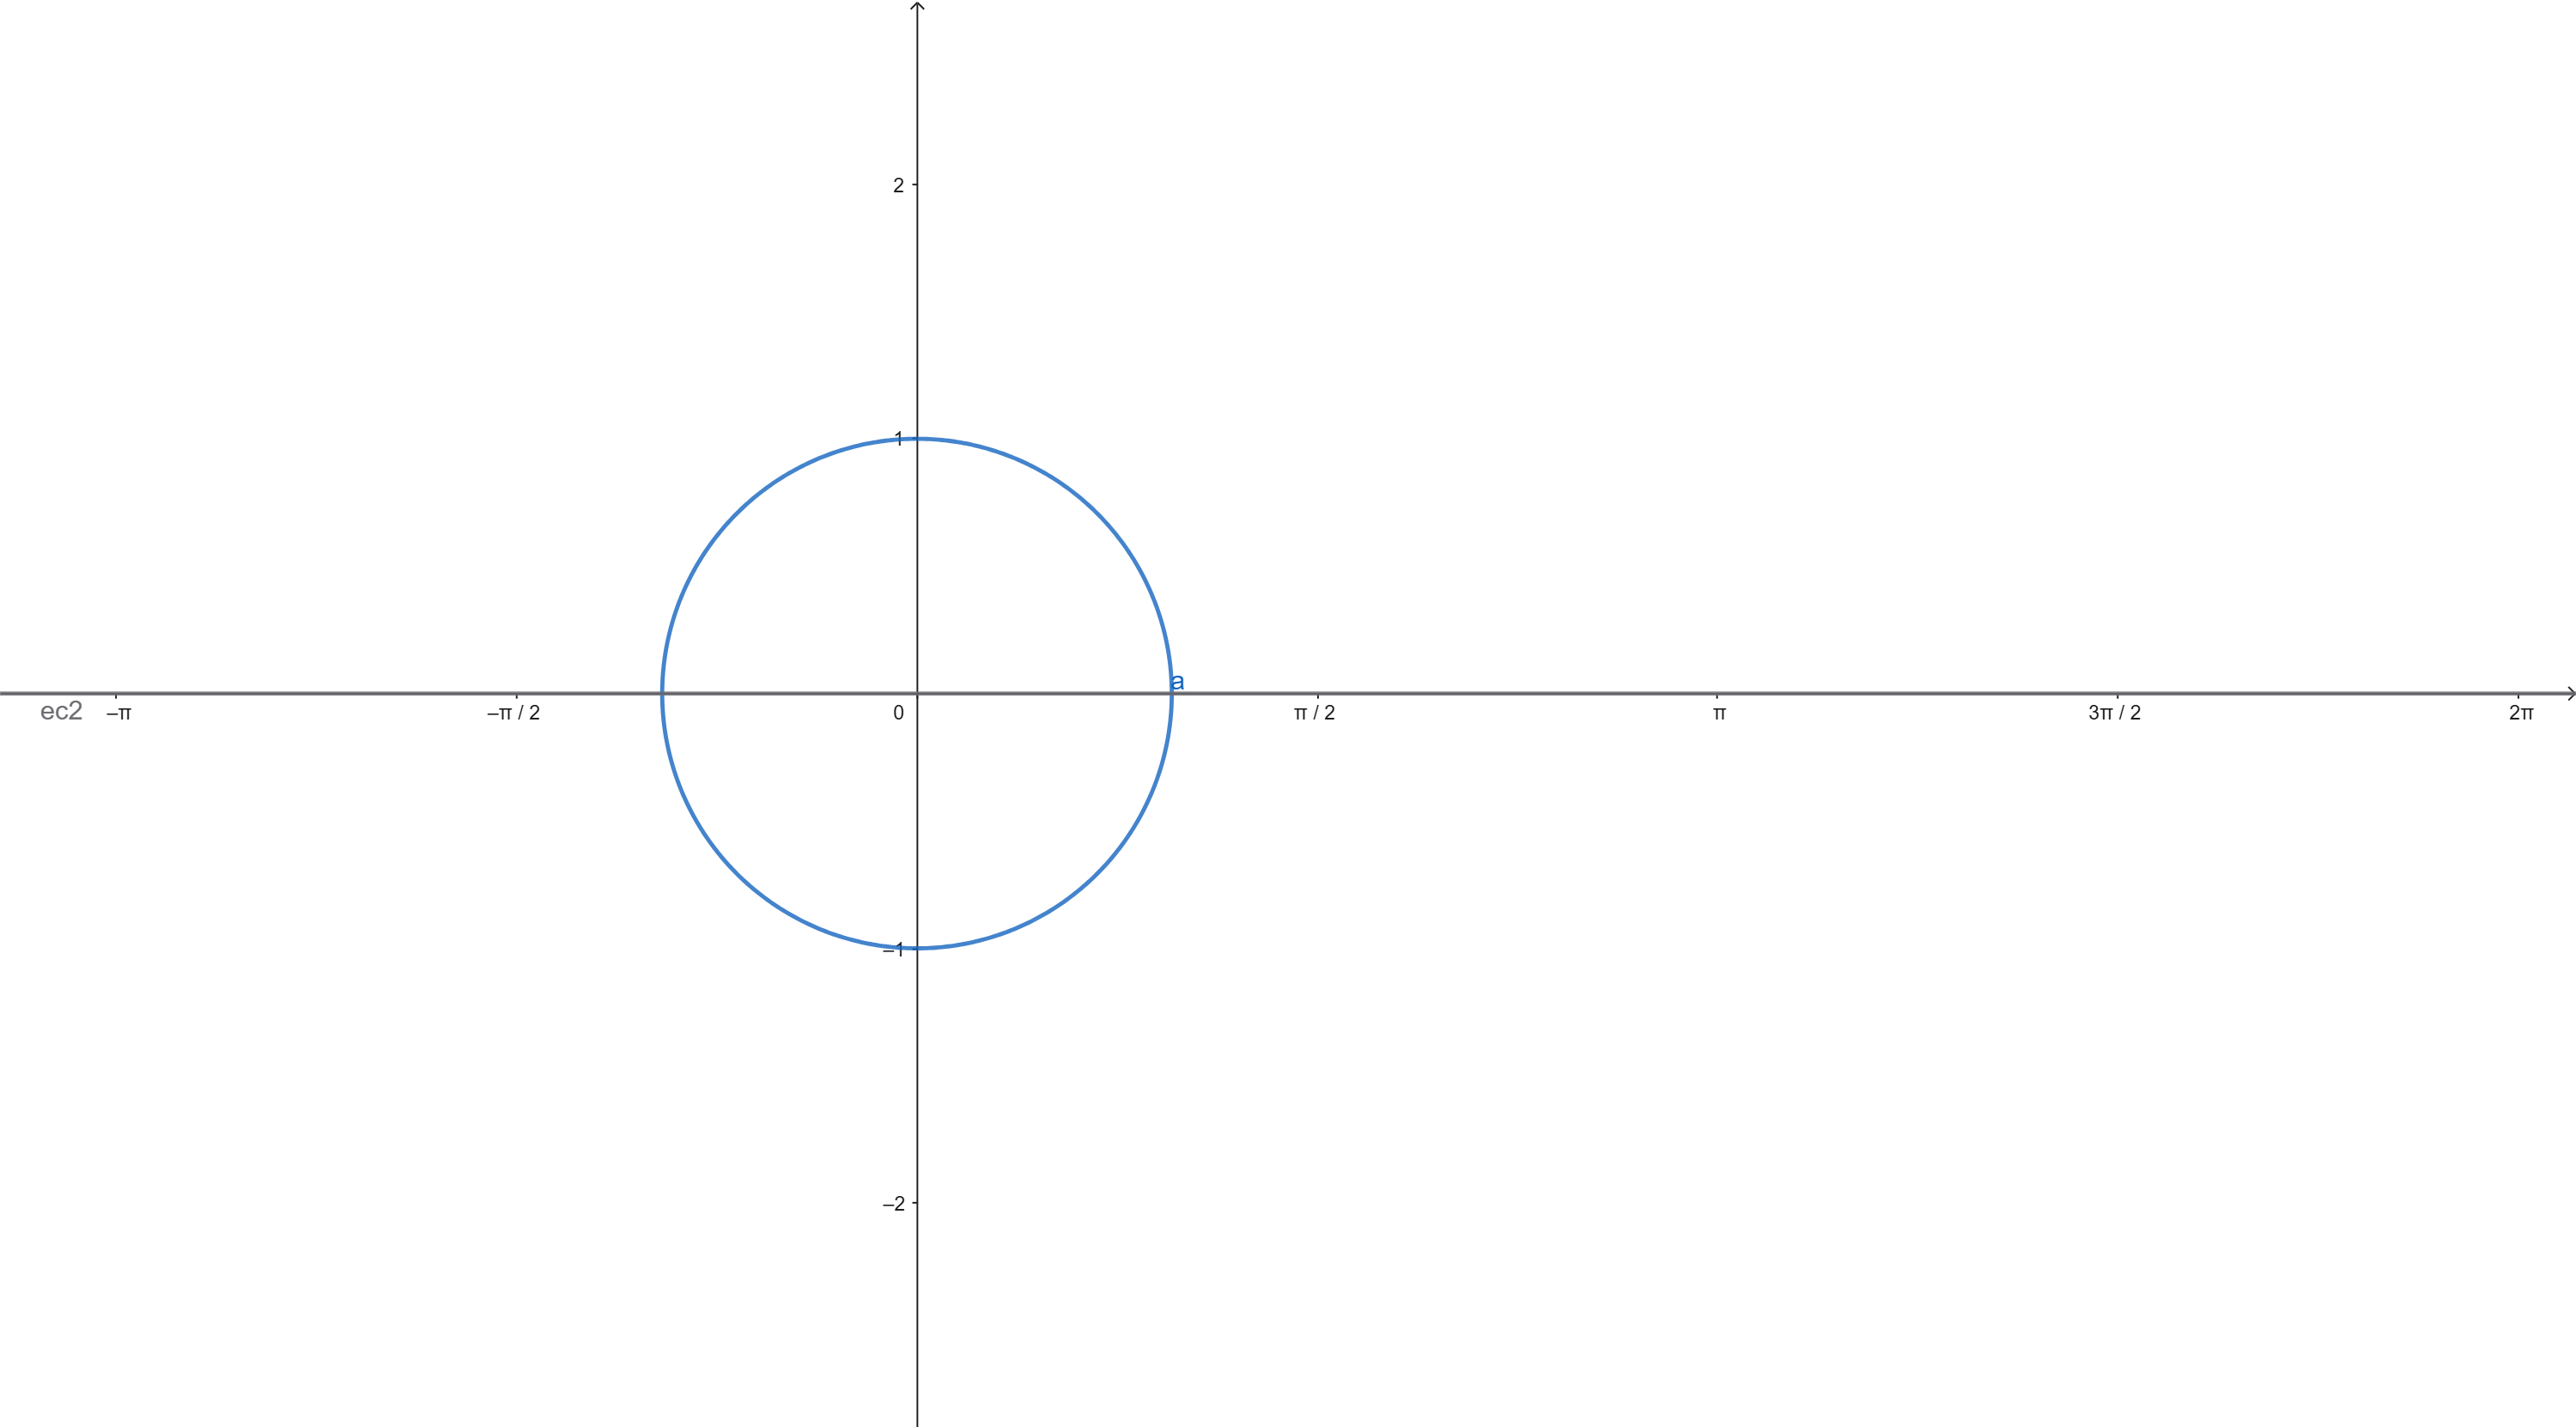
\includegraphics[width=0.55\textwidth]{Apendices/curve.png}
  \caption{Curva paramétrica continua del tiempo sobre el círculo unitario}
  \caption*{GeoGebra: Generación de la curva mediante las expresiones: \newline
  \texttt{x(t) = cos(2$\pi$ * t / 86400)}, \quad
  \texttt{y(t) = sin(2$\pi$ * t / 86400)}, \quad
  \texttt{Curve(x(t), y(t), t, 0, 86400)}}
  \caption*{La figura muestra una curva paramétrica continua que representa el tiempo sobre el círculo unitario mediante funciones trigonométricas. Cada instante se proyecta como un punto único definido por \( x(t) = \cos\left(\frac{2\pi t}{86400}\right) \) y \( y(t) = \sin\left(\frac{2\pi t}{86400}\right) \), donde \( t \) es el número de segundos desde las 00:00. Esta codificación garantiza continuidad angular, permitiendo que modelos de simulación o aprendizaje automático interpreten correctamente la naturaleza cíclica del tiempo sin ambigüedades en los extremos del día.}
  \label{fig:curva-tiempo-circular}
\end{figure}
\uextra{Apendice}{Verificación del sistema de monitoreo acústico}

{\small
  \begin{longtable}[c]{c p{3.5cm} p{2.2cm} p{2.2cm} p{3.5cm}}
    \hline
    \textbf{Requerimiento} & \textbf{Descripción}                                                                                    & \textbf{Entrada}                                                  & \textbf{Salida}                                                       & \textbf{Criterio de Aceptación}                                                       \\
    \hline
    \endfirsthead

    \hline
    \textbf{Requerimiento} & \textbf{Descripción}                                                                                    & \textbf{Entrada}                                                  & \textbf{Salida}                                                       & \textbf{Criterio de Aceptación}                                                       \\
    \hline
    \endhead
    \endfoot
    \endlastfoot

    R1                     & Captura continua del audio ambiental a través de micrófonos.                                            & Señales de audio del entorno a través del hardware del micrófono. & Eventos discretos etiquedados del audio.                              & El sistema debe estar activo y registrando datos en todo momento.                     \\
    \addlinespace
    R2                     & Procesamiento del audio para clasificarlo en eventos sonoros predefinidos.                              & Flujo de datos de audio.                                          & Clasificación del sonido (ej. voz, silencio, golpe).                  & El sistema debe etiquetar correctamente la señal de audio que recibe en todo momento. \\
    \addlinespace
    R3                     & El sistema debe conocer en todo momento el estado de actividad del entorno.                             & Señal de audio.                                                   & Hay ruido o silencio.                                                 & El sistema reconoce cuando hay ruido o silencio.                                      \\
    \addlinespace
    R4                     & Comparación de la actividad en tiempo real con el perfil de normalidad para detectar patrones anómalos. & Secuencia de eventos en tiempo real                               & Identificación de una anomalía o evento atípico.                      & Detectar si una secuencia de eventos es normal o anómala.                             \\
    \addlinespace
    R5                     & El sistema realiza una consulta verbal al usuario al detectar una anomalía.                             & Señal de audio.                                                   & Emisión de una pregunta de voz pregrabada (ej. ``¿Está todo bien?''). & El sistema consulta el estado del usuario antes de enviar una alerta.                 \\
    \addlinespace
    R6                     & Permitir cancelar una alerta de emergencia por comando de voz.                                          & Respuesta de voz del usuario (ej. ``Estoy bien'').                & No se envía alerta.                                                   & El sistema cancela la alerta.                                                         \\
    \addlinespace
    R7                     & El sistema envía notificaciones de emergencia si la anomalía es crítica o el usuario no responde.       & Falta de respuesta del usuario o gravedad de la anomalía          & Envío de notificaciones.                                              & El sistema es capaz de enviar una alerta sin la intervención del usuario.             \\
    \bottomrule
    \addlinespace

    \caption{Requerimientos del sistema acústico}
    \label{tab:requerimientos_sistema_acustico}
  \end{longtable}
}


\clearpage

% Guardar el número de página actual
\newcounter{pags}
\setcounter{pags}{\value{page}}

\pagestyle{plain}

\pagenumbering{roman}
\setcounter{page}{\value{pags}}
\tableofcontents
\clearpage
\listoftables
\clearpage
\listoffigures
\clearpage
\listofmyequations
\clearpage

\newcounter{abstractpage}
\setcounter{abstractpage}{\value{page}}

% Keywords command
\providecommand{\keywords}[1]
{
  \small
  \textbf{\textit{Palabras clave---}} #1
}

\begin{abstract}
  \thispagestyle{plain}
  \setcounter{page}{\value{abstractpage}}
  Este trabajo presenta el desarrollo de un sistema de monitoreo acústico basado en inteligencia artificial, orientado a clasificar sonidos ambientales y generar alertas de emergencia al identificar eventos anómalos en tiempo real que podrían implicar que individuos se encuentren vulnerables. La creciente adopción de tecnologías para el hogar inteligente crea el ecosistema ideal para desarrollar soluciones avanzadas de monitoreo no invasivo. En este marco, el proyecto aborda la detección de eventos críticos, como cambios en la rutina o gritos de auxilio, con el fin de ofrecer una herramienta de alerta temprana ante situaciones de vulnerabilidad que, en el pasado, han derivado en tragedias por falta de detección. El sistema fue desarrollado utilizando dispositivos Edge como Raspberry Pi, integrando modelos preentrenados como YAMNet para clasificación de sonidos y Vosk para detección de palabras clave con modelos propios que perfilan el comportamiento acústico con Isolation Forest, LSTM y Transformers. La metodología empleada está basada en el modelo de desarrollo en espiral, lo cual permitió ciclos iterativos de análisis, diseño, implementación y validación, adaptándose a desafíos técnicos como la variabilidad del entorno sonoro y las limitaciones de hardware. En el desarrollo, se exploraron distintos enfoques: se evaluaron modelos de series temporales como ARIMA y Prophet, así como cadenas de Markov para analizar anomalías basadas en cambios de estado. Se determinó que estos modelos, si bien podían identificar ciertos eventos puntuales, carecían de la robustez necesaria para modelar la complejidad del entorno acústico en tiempo real. Los resultados evidencian que el sistema es capaz de identificar patrones anómalos de sonido en tiempo real y generar notificaciones automáticas a contactos de emergencia. La solución, cumple con normas legales sobre privacidad al no almacenar audios y procesar todo localmente. Se concluye que este sistema representa una herramienta ética para el monitoreo de entornos domésticos, alineándose con los Objetivos de Desarrollo Sostenible en salud, bienestar e inclusión tecnológica.

  \keywords{alertas de emergencia, dispositivos Edge, inteligencia artificial, monitoreo acústico, Raspberry Pi.}
\end{abstract}

\clearpage


\fancypagestyle{plain}{
  \fancyhf{}
  \fancyhead[R]{\thepage}
}
\pagestyle{plain}
\pagenumbering{arabic}
\setcounter{page}{1}
\phantomsection
\chapter*{Introducción}
\addcontentsline{toc}{chapter}{Introducción}

Este trabajo aborda el desarrollo de un sistema distribuido que, mediante el uso de inteligencia artificial, permite la detección de anomalías acústicas como herramienta de apoyo para la alerta temprana ante posibles emergencias. El sistema está enfocado en servir no solo a personas mayores o con discapacidades, sino también a cualquier individuo que se encuentre en una condición de vulnerabilidad. Su funcionamiento se basa en dispositivos que primero clasifican los sonidos ambientales en tiempo real para, posteriormente, analizar la secuencia de dichas clasificaciones. Este análisis permite al sistema caracterizar el comportamiento acústico “normal” de un entorno y, en consecuencia, identificar eventos que se desvían de esa normalidad para generar una alerta a contactos predefinidos. La importancia de este proyecto radica en su capacidad de alertar sobre situaciones anormales que podrían indicar una situación de emergencia, ofreciendo un sistema de alerta temprana que respeta la privacidad. Además, tiene el potencial de beneficiar a familias, cuidadores e instituciones y facilitar una intervención más oportuna de los servicios de emergencia, incluso en casos de violencia doméstica o el monitoreo de personas con depresión. A través de la identificación de situaciones anormales y la emisión de alertas, este sistema contribuye a una mejor calidad de vida.

Para el desarrollo del sistema, se empleó una metodología basada en el modelo de desarrollo en espiral, que permite un enfoque iterativo y flexible. Cada ciclo del proceso abarca fases de planificación, análisis de riesgos, desarrollo y evaluación, permitiendo ajustes continuos en el diseño y la implementación del sistema. Esta metodología es adecuada para proyectos con incertidumbre, ya que facilita la evolución del sistema según la retroalimentación obtenida, asegurando su mejora progresiva a lo largo del desarrollo.

El presente trabajo está estructurado en cinco capítulos, En el Capítulo I, referido al Planteamiento del Problema, se describe la problemática, se establecen los objetivos, justificación, alcance y limitaciones del proyecto. En el Capítulo II, se expone el Marco Teórico donde se recopilan los antecedentes y las bases teóricas que sustentan el trabajo. En el Capítulo III, se presenta el Marco Metodológico, que describe el tipo de investigación, técnicas e instrumentos de recolección de datos, metodología de desarrollo y el procedimiento metodológico. En el Capítulo IV, se expone el Desarrollo y Resultados, donde se describe como el procedimiento metodológico dio respuesta a cada uno de los objetivos planteados, y en el Capítulo V, se presentan las conclusiones y recomendaciones sobre el trabajo realizado. Finalmente se listan las referencias bibliográficas utilizadas, seguidas de los anexos y apéndices.

\clearpage

\titleformat{\chapter}
{\normalfont\fontsize{12}{15}\centering}{Anexos \thechapter.}{0.3em}{}[]

\clearpage
\thispagestyle{empty}
\begin{center}
  \vspace*{\fill}
  \phantomsection
  Apéndices
  \addcontentsline{toc}{chapter}{Anexos}
  \vspace*{\fill}
\end{center}
\clearpage

\appendix
% \uextra{Apendice}{Dispositivo Raspberry Pi 4 Model B}
% \begin{figure}[ht!]
%   \centering
%   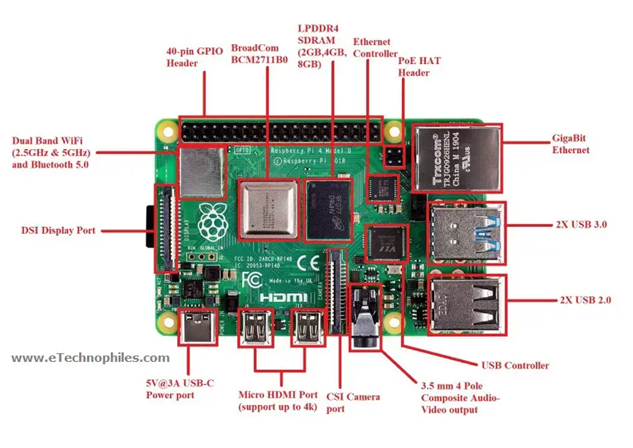
\includegraphics[width=0.95\textwidth]{Anexos/1.arquitectura-raspberry.png}
%   \caption{Arquitectura del Raspberry Pi 4 Model B}
%   \label{fig:raspberry-architecture}
% \end{figure}

\uextra{Apendice}{Representación cíclica del tiempo mediante funciones trigonométricas}
\begin{figure}[ht!]
  \centering
  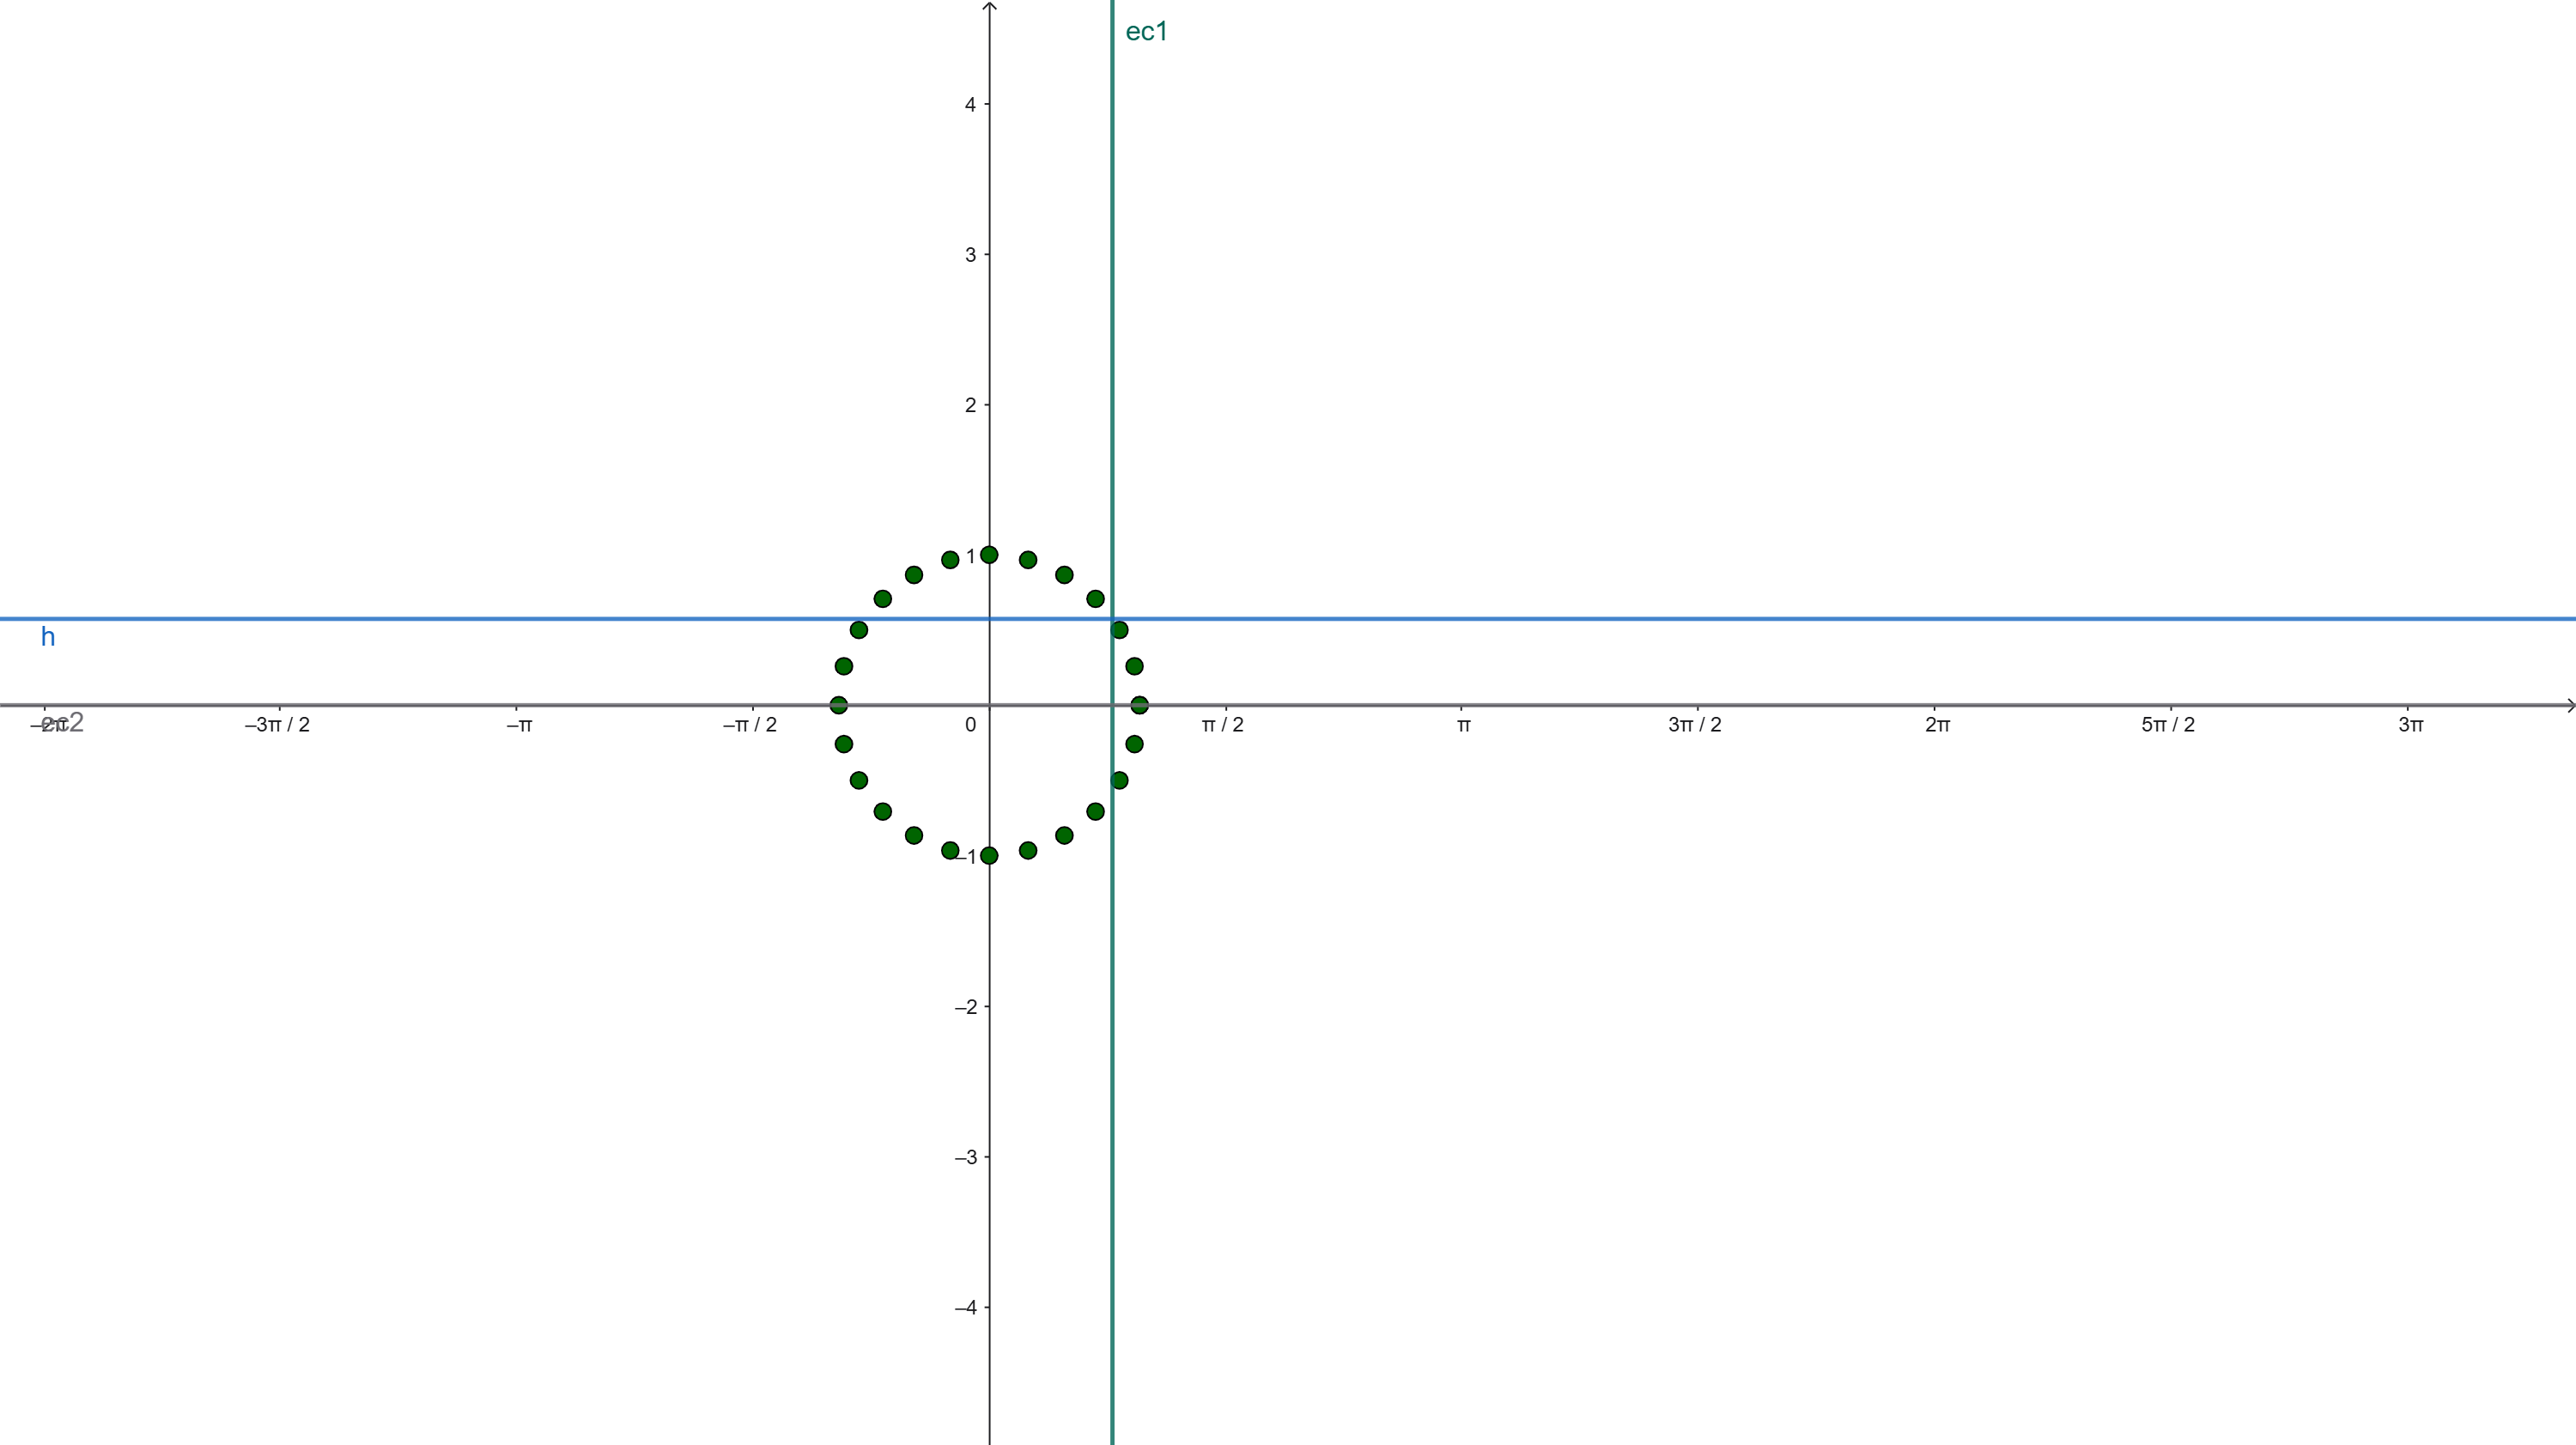
\includegraphics[width=0.55\textwidth]{Apendices/rc.png}
  \caption{Visualización discreta del comportamiento cíclico del tiempo} 
  \caption*{GeoGebra: Generación de puntos discretos sobre la circunferencia usando la expresión: \newline
  \texttt{Sequence((cos(2$\pi$ * n / 86400), sin(2$\pi$ * n / 86400)), n, 0, 86400, 3600)}}
  \caption*{La figura incluye dos líneas auxiliares que recorren la circunferencia: una horizontal (coseno) y una vertical (seno), generadas dinámicamente mediante un deslizador \( t \) con paso de 600 segundos. Estas líneas intersectan en el punto \( (x, y) \), representando la posición temporal proyectada en coordenadas trigonométricas.}
  \label{fig:representacion-ciclica-tiempo}
\end{figure}

\begin{figure}[ht!]
  \centering
  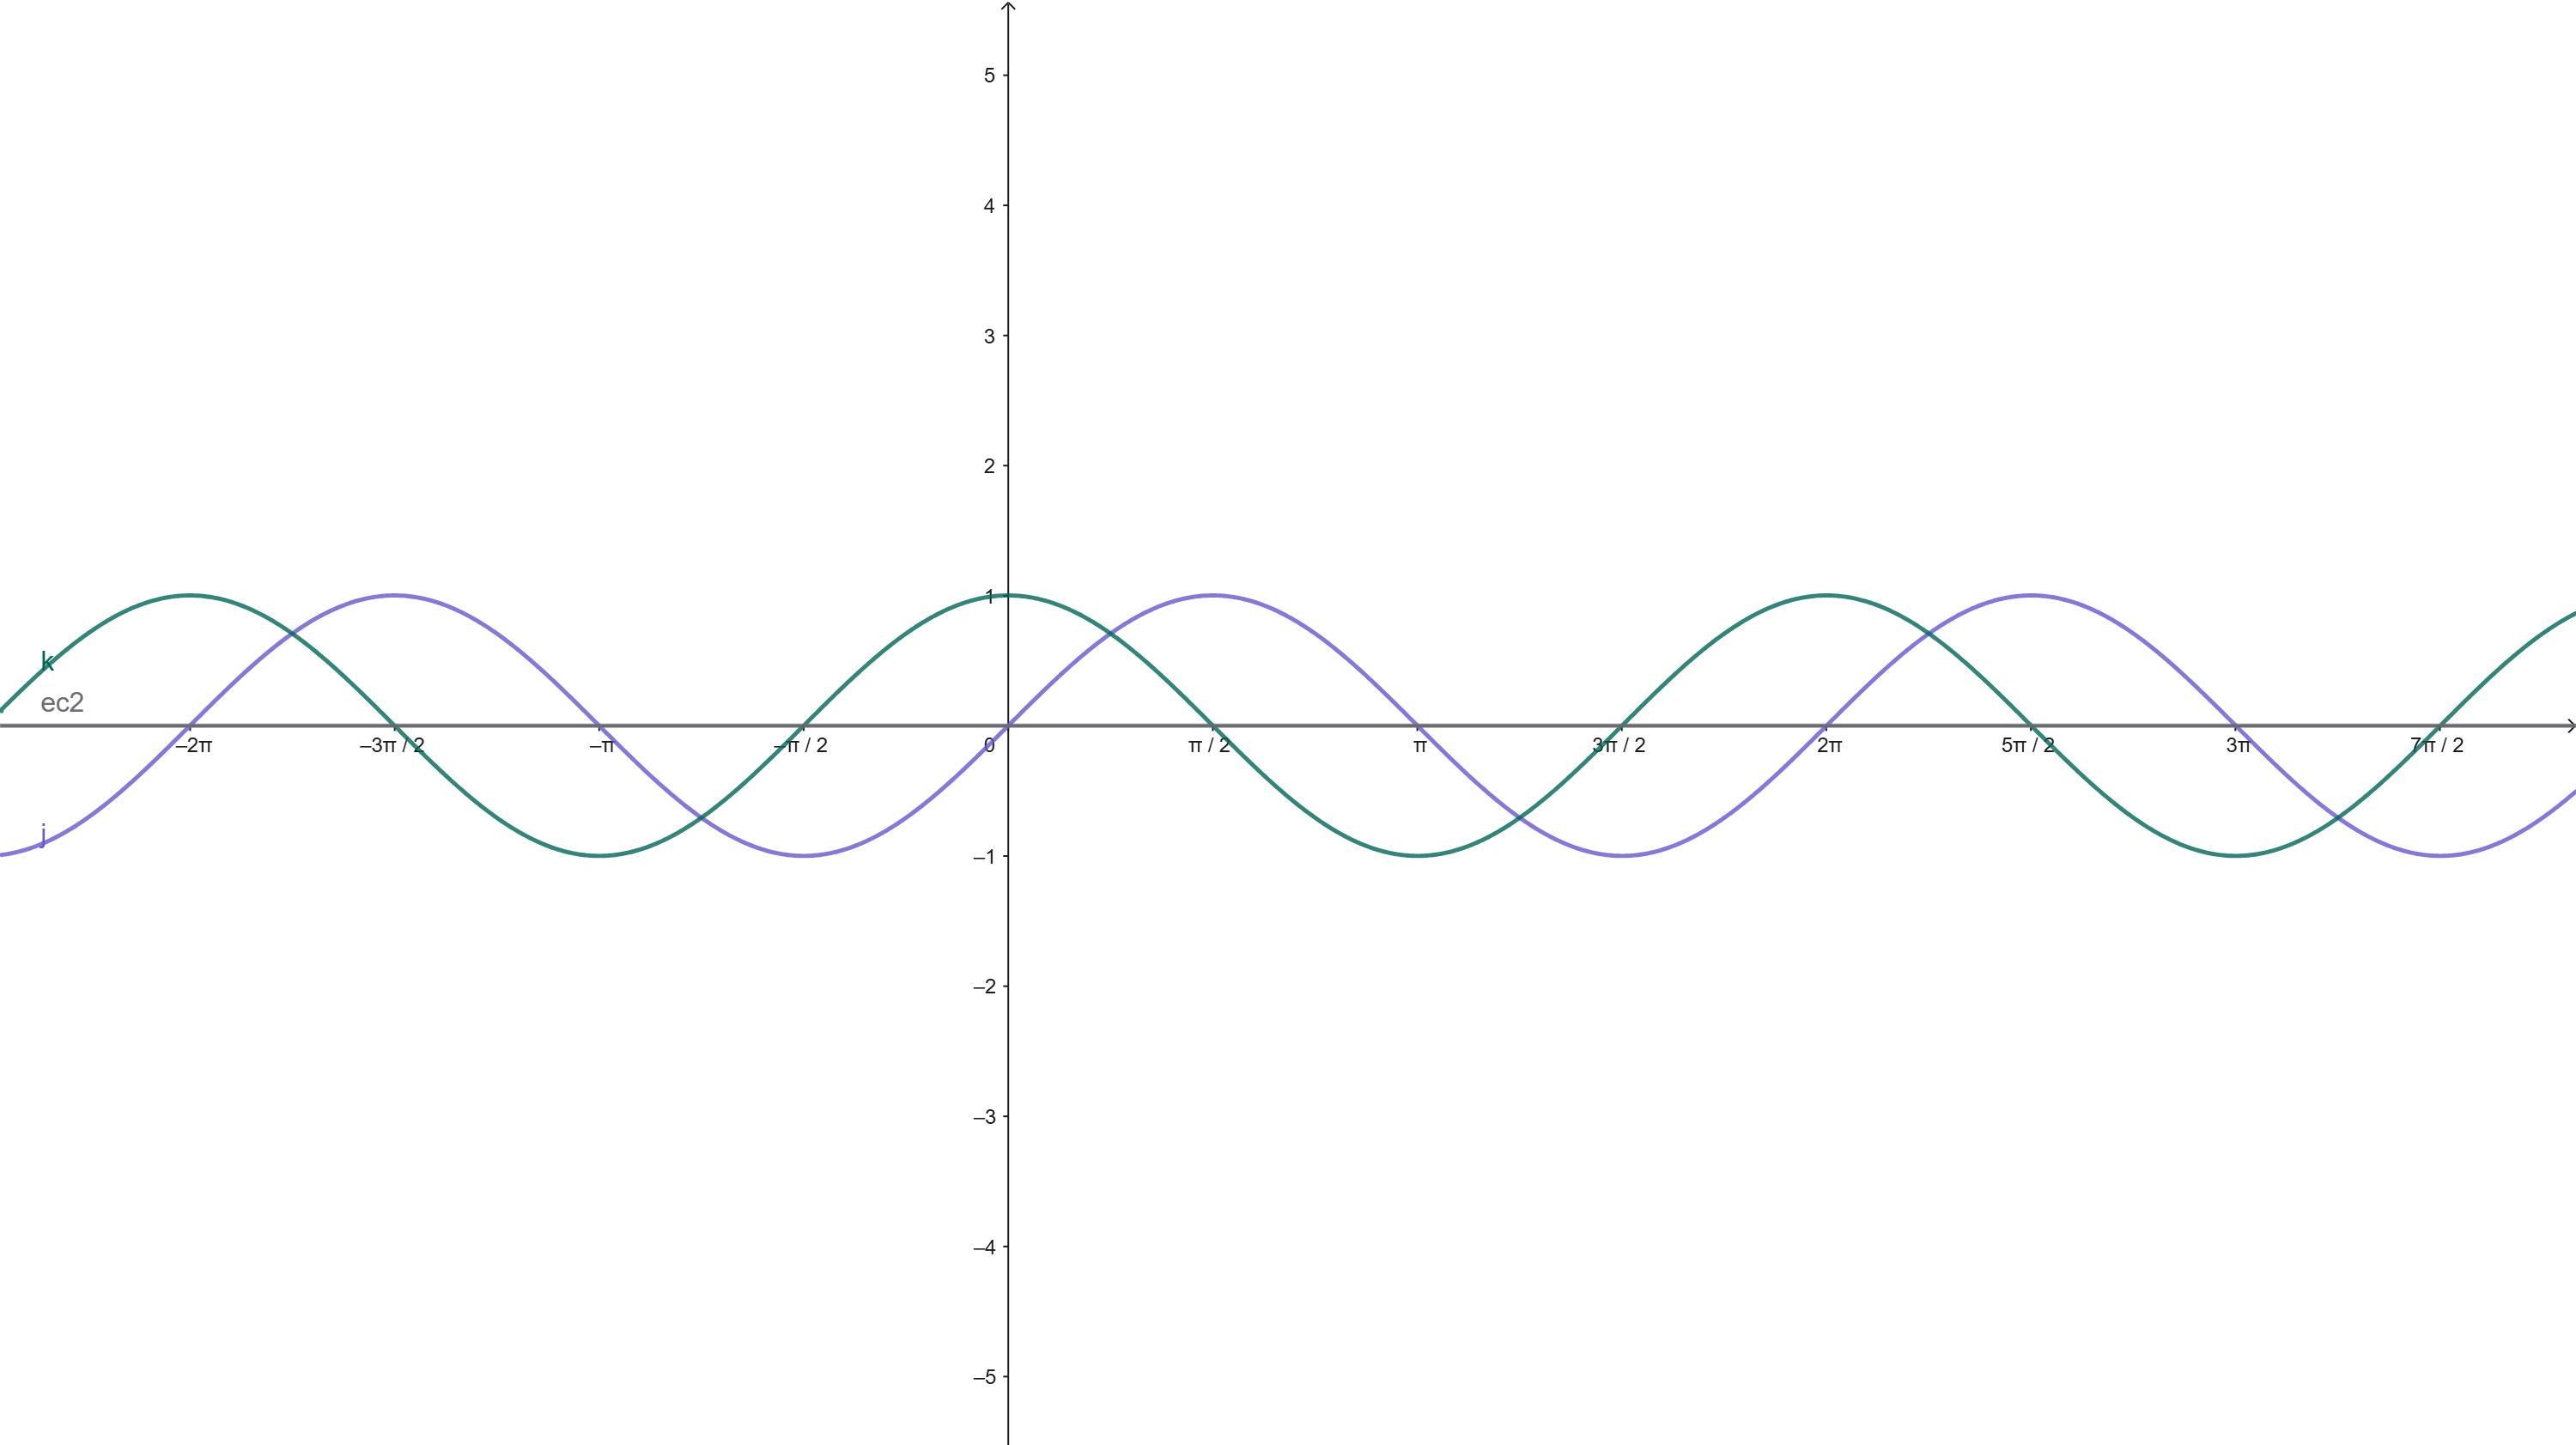
\includegraphics[width=0.55\textwidth]{Apendices/sencos.png}
  \caption{Visualización de las funciones seno y coseno  } 
  \caption*{GeoGebra: Generación de las funciones seno y coseno usando las expresiones: \newline
  \texttt{Sequence((x, sin(x)), x, 0, 2$\pi$, $\pi$/6)} y \newline
  \texttt{Sequence((x, cos(x)), x, 0, 2$\pi$, $\pi$/6)}}
  \label{fig: seno-coseno}
\end{figure}

\begin{figure}[ht!]
  \centering
  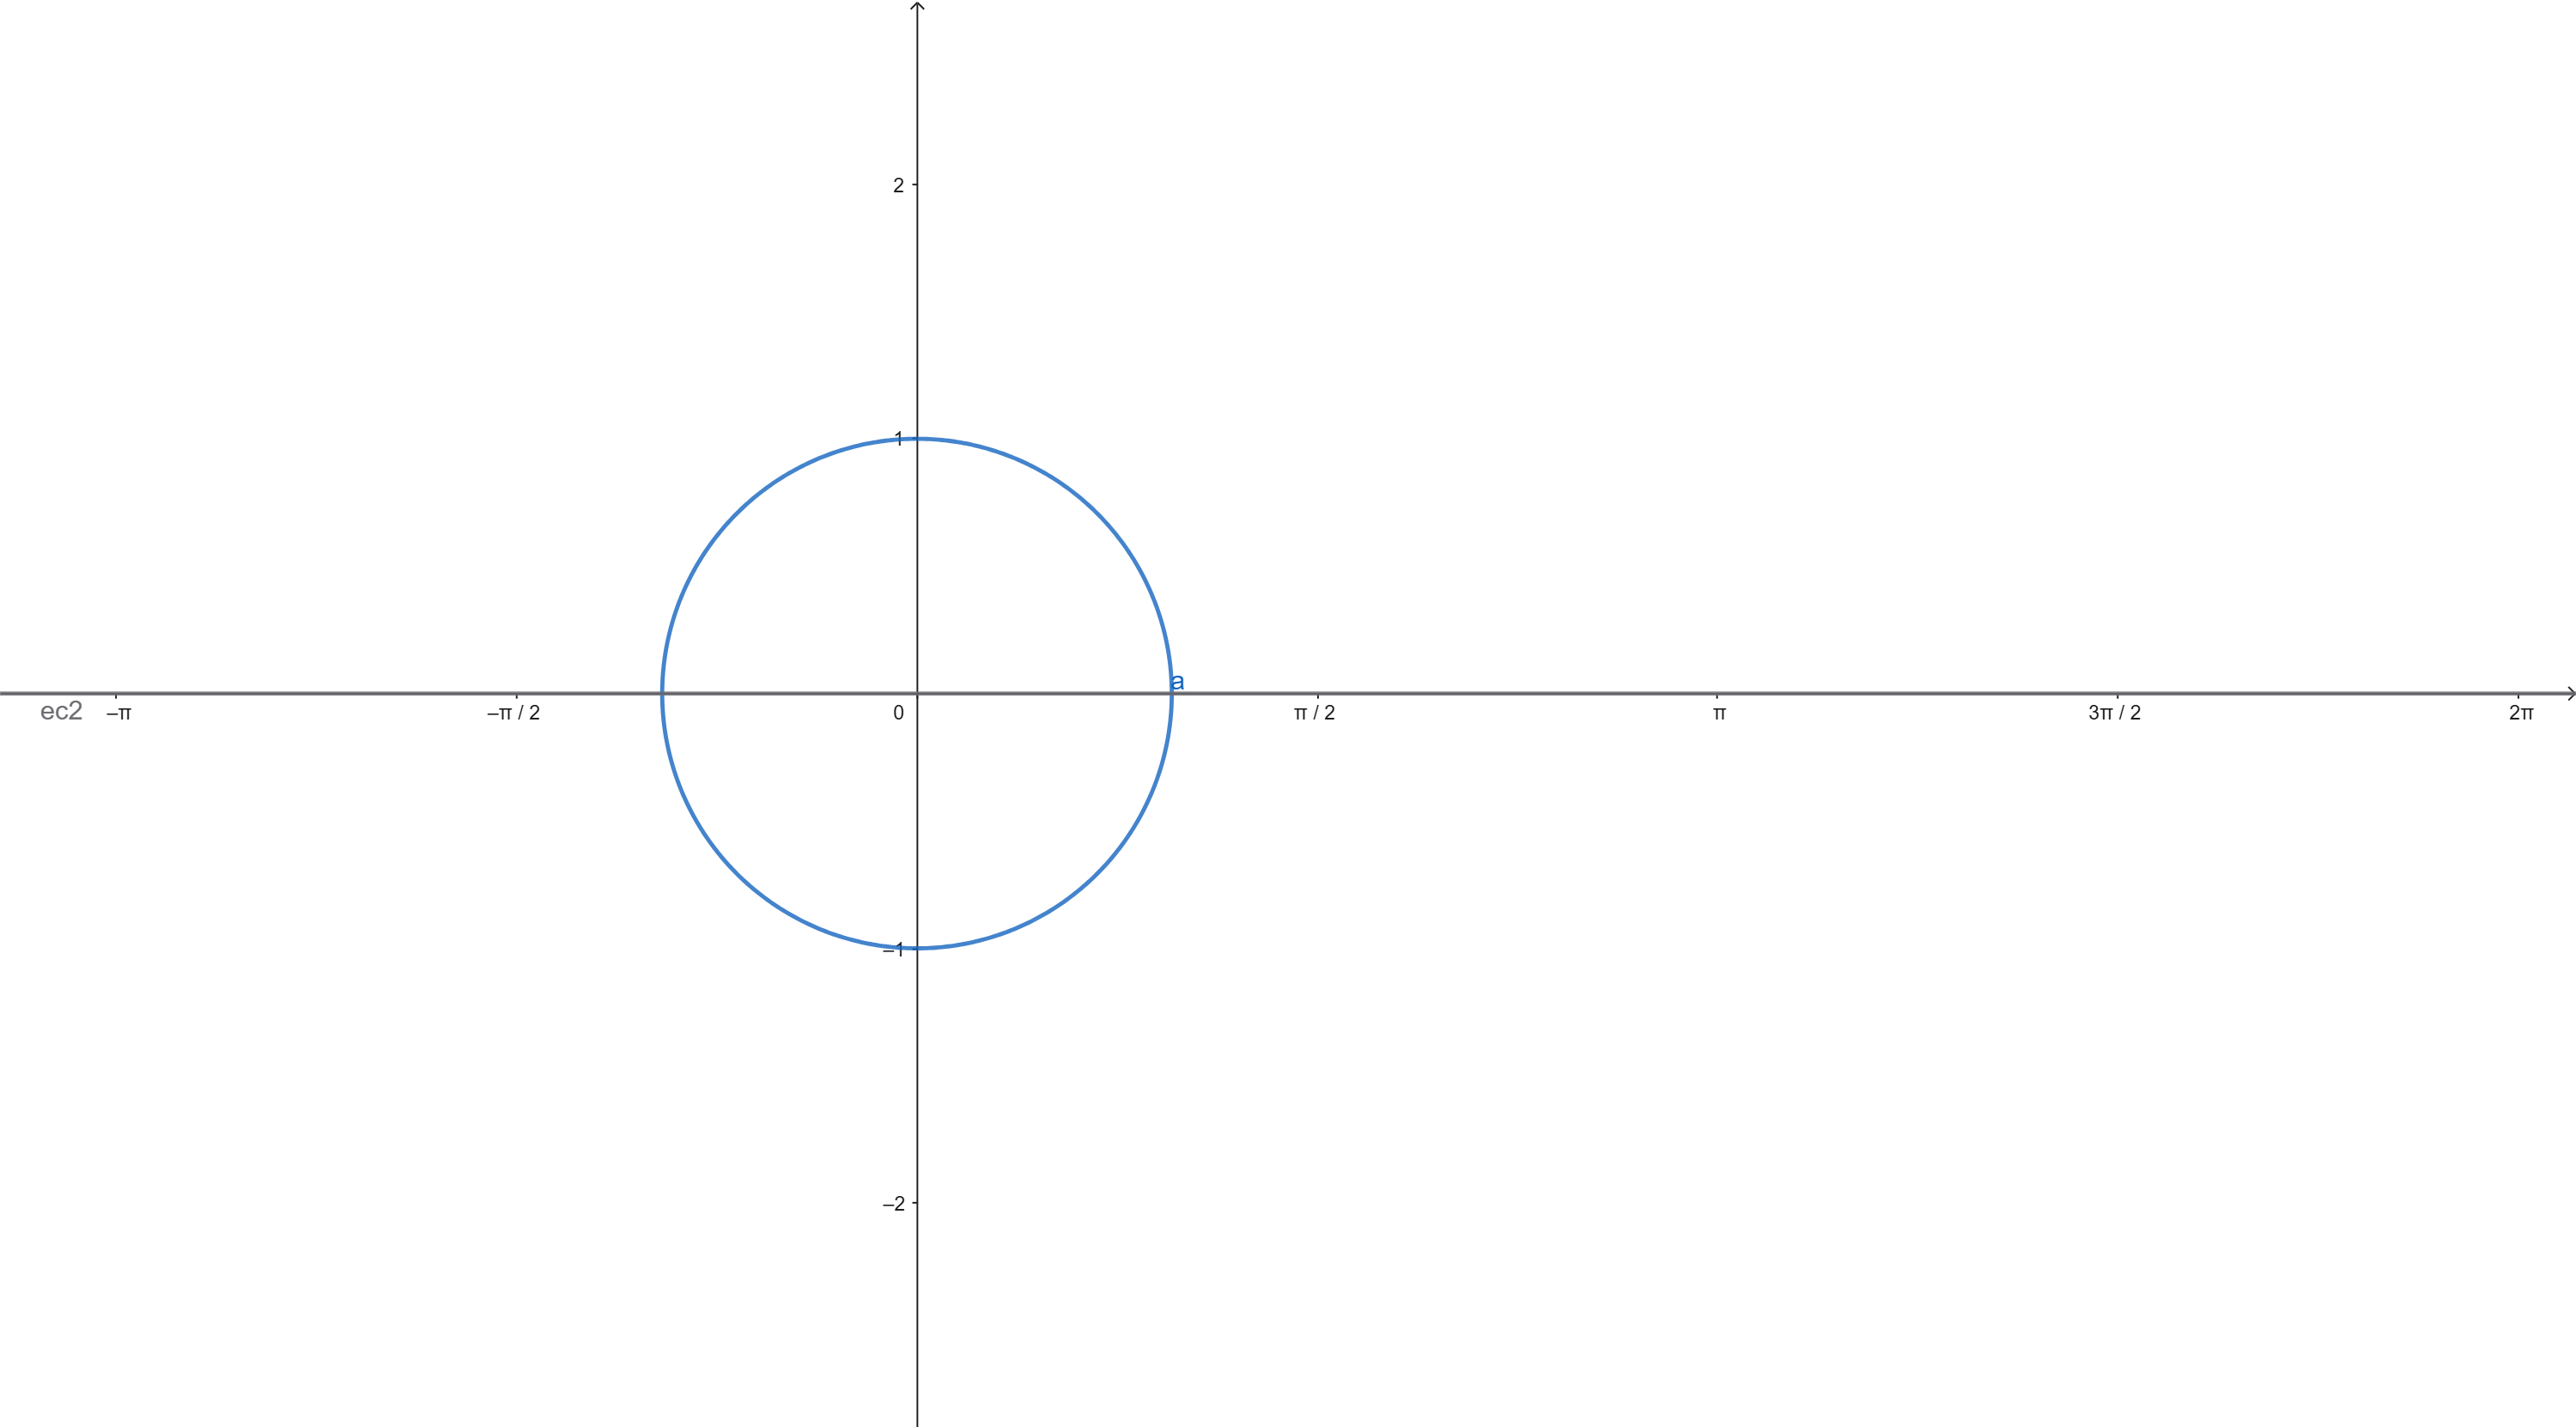
\includegraphics[width=0.55\textwidth]{Apendices/curve.png}
  \caption{Curva paramétrica continua del tiempo sobre el círculo unitario}
  \caption*{GeoGebra: Generación de la curva mediante las expresiones: \newline
  \texttt{x(t) = cos(2$\pi$ * t / 86400)}, \quad
  \texttt{y(t) = sin(2$\pi$ * t / 86400)}, \quad
  \texttt{Curve(x(t), y(t), t, 0, 86400)}}
  \caption*{La figura muestra una curva paramétrica continua que representa el tiempo sobre el círculo unitario mediante funciones trigonométricas. Cada instante se proyecta como un punto único definido por \( x(t) = \cos\left(\frac{2\pi t}{86400}\right) \) y \( y(t) = \sin\left(\frac{2\pi t}{86400}\right) \), donde \( t \) es el número de segundos desde las 00:00. Esta codificación garantiza continuidad angular, permitiendo que modelos de simulación o aprendizaje automático interpreten correctamente la naturaleza cíclica del tiempo sin ambigüedades en los extremos del día.}
  \label{fig:curva-tiempo-circular}
\end{figure}
\uextra{Apendice}{Verificación del sistema de monitoreo acústico}

{\small
  \begin{longtable}[c]{c p{3.5cm} p{2.2cm} p{2.2cm} p{3.5cm}}
    \hline
    \textbf{Requerimiento} & \textbf{Descripción}                                                                                    & \textbf{Entrada}                                                  & \textbf{Salida}                                                       & \textbf{Criterio de Aceptación}                                                       \\
    \hline
    \endfirsthead

    \hline
    \textbf{Requerimiento} & \textbf{Descripción}                                                                                    & \textbf{Entrada}                                                  & \textbf{Salida}                                                       & \textbf{Criterio de Aceptación}                                                       \\
    \hline
    \endhead
    \endfoot
    \endlastfoot

    R1                     & Captura continua del audio ambiental a través de micrófonos.                                            & Señales de audio del entorno a través del hardware del micrófono. & Eventos discretos etiquedados del audio.                              & El sistema debe estar activo y registrando datos en todo momento.                     \\
    \addlinespace
    R2                     & Procesamiento del audio para clasificarlo en eventos sonoros predefinidos.                              & Flujo de datos de audio.                                          & Clasificación del sonido (ej. voz, silencio, golpe).                  & El sistema debe etiquetar correctamente la señal de audio que recibe en todo momento. \\
    \addlinespace
    R3                     & El sistema debe conocer en todo momento el estado de actividad del entorno.                             & Señal de audio.                                                   & Hay ruido o silencio.                                                 & El sistema reconoce cuando hay ruido o silencio.                                      \\
    \addlinespace
    R4                     & Comparación de la actividad en tiempo real con el perfil de normalidad para detectar patrones anómalos. & Secuencia de eventos en tiempo real                               & Identificación de una anomalía o evento atípico.                      & Detectar si una secuencia de eventos es normal o anómala.                             \\
    \addlinespace
    R5                     & El sistema realiza una consulta verbal al usuario al detectar una anomalía.                             & Señal de audio.                                                   & Emisión de una pregunta de voz pregrabada (ej. ``¿Está todo bien?''). & El sistema consulta el estado del usuario antes de enviar una alerta.                 \\
    \addlinespace
    R6                     & Permitir cancelar una alerta de emergencia por comando de voz.                                          & Respuesta de voz del usuario (ej. ``Estoy bien'').                & No se envía alerta.                                                   & El sistema cancela la alerta.                                                         \\
    \addlinespace
    R7                     & El sistema envía notificaciones de emergencia si la anomalía es crítica o el usuario no responde.       & Falta de respuesta del usuario o gravedad de la anomalía          & Envío de notificaciones.                                              & El sistema es capaz de enviar una alerta sin la intervención del usuario.             \\
    \bottomrule
    \addlinespace

    \caption{Requerimientos del sistema acústico}
    \label{tab:requerimientos_sistema_acustico}
  \end{longtable}
}

\titleformat{\chapter}
{\normalfont\fontsize{12}{15}\centering}{Anexos \thechapter.}{0.3em}{}[]

\clearpage
\thispagestyle{empty}
\begin{center}
  \vspace*{\fill}
  \phantomsection
  Apéndices
  \addcontentsline{toc}{chapter}{Anexos}
  \vspace*{\fill}
\end{center}
\clearpage

\appendix
% \uextra{Apendice}{Dispositivo Raspberry Pi 4 Model B}
% \begin{figure}[ht!]
%   \centering
%   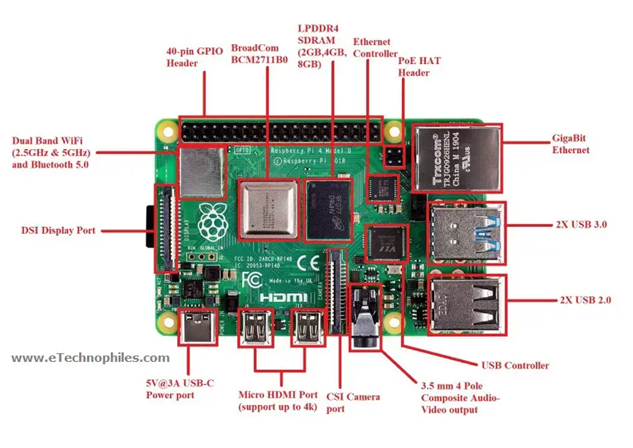
\includegraphics[width=0.95\textwidth]{Anexos/1.arquitectura-raspberry.png}
%   \caption{Arquitectura del Raspberry Pi 4 Model B}
%   \label{fig:raspberry-architecture}
% \end{figure}

\uextra{Apendice}{Representación cíclica del tiempo mediante funciones trigonométricas}
\begin{figure}[ht!]
  \centering
  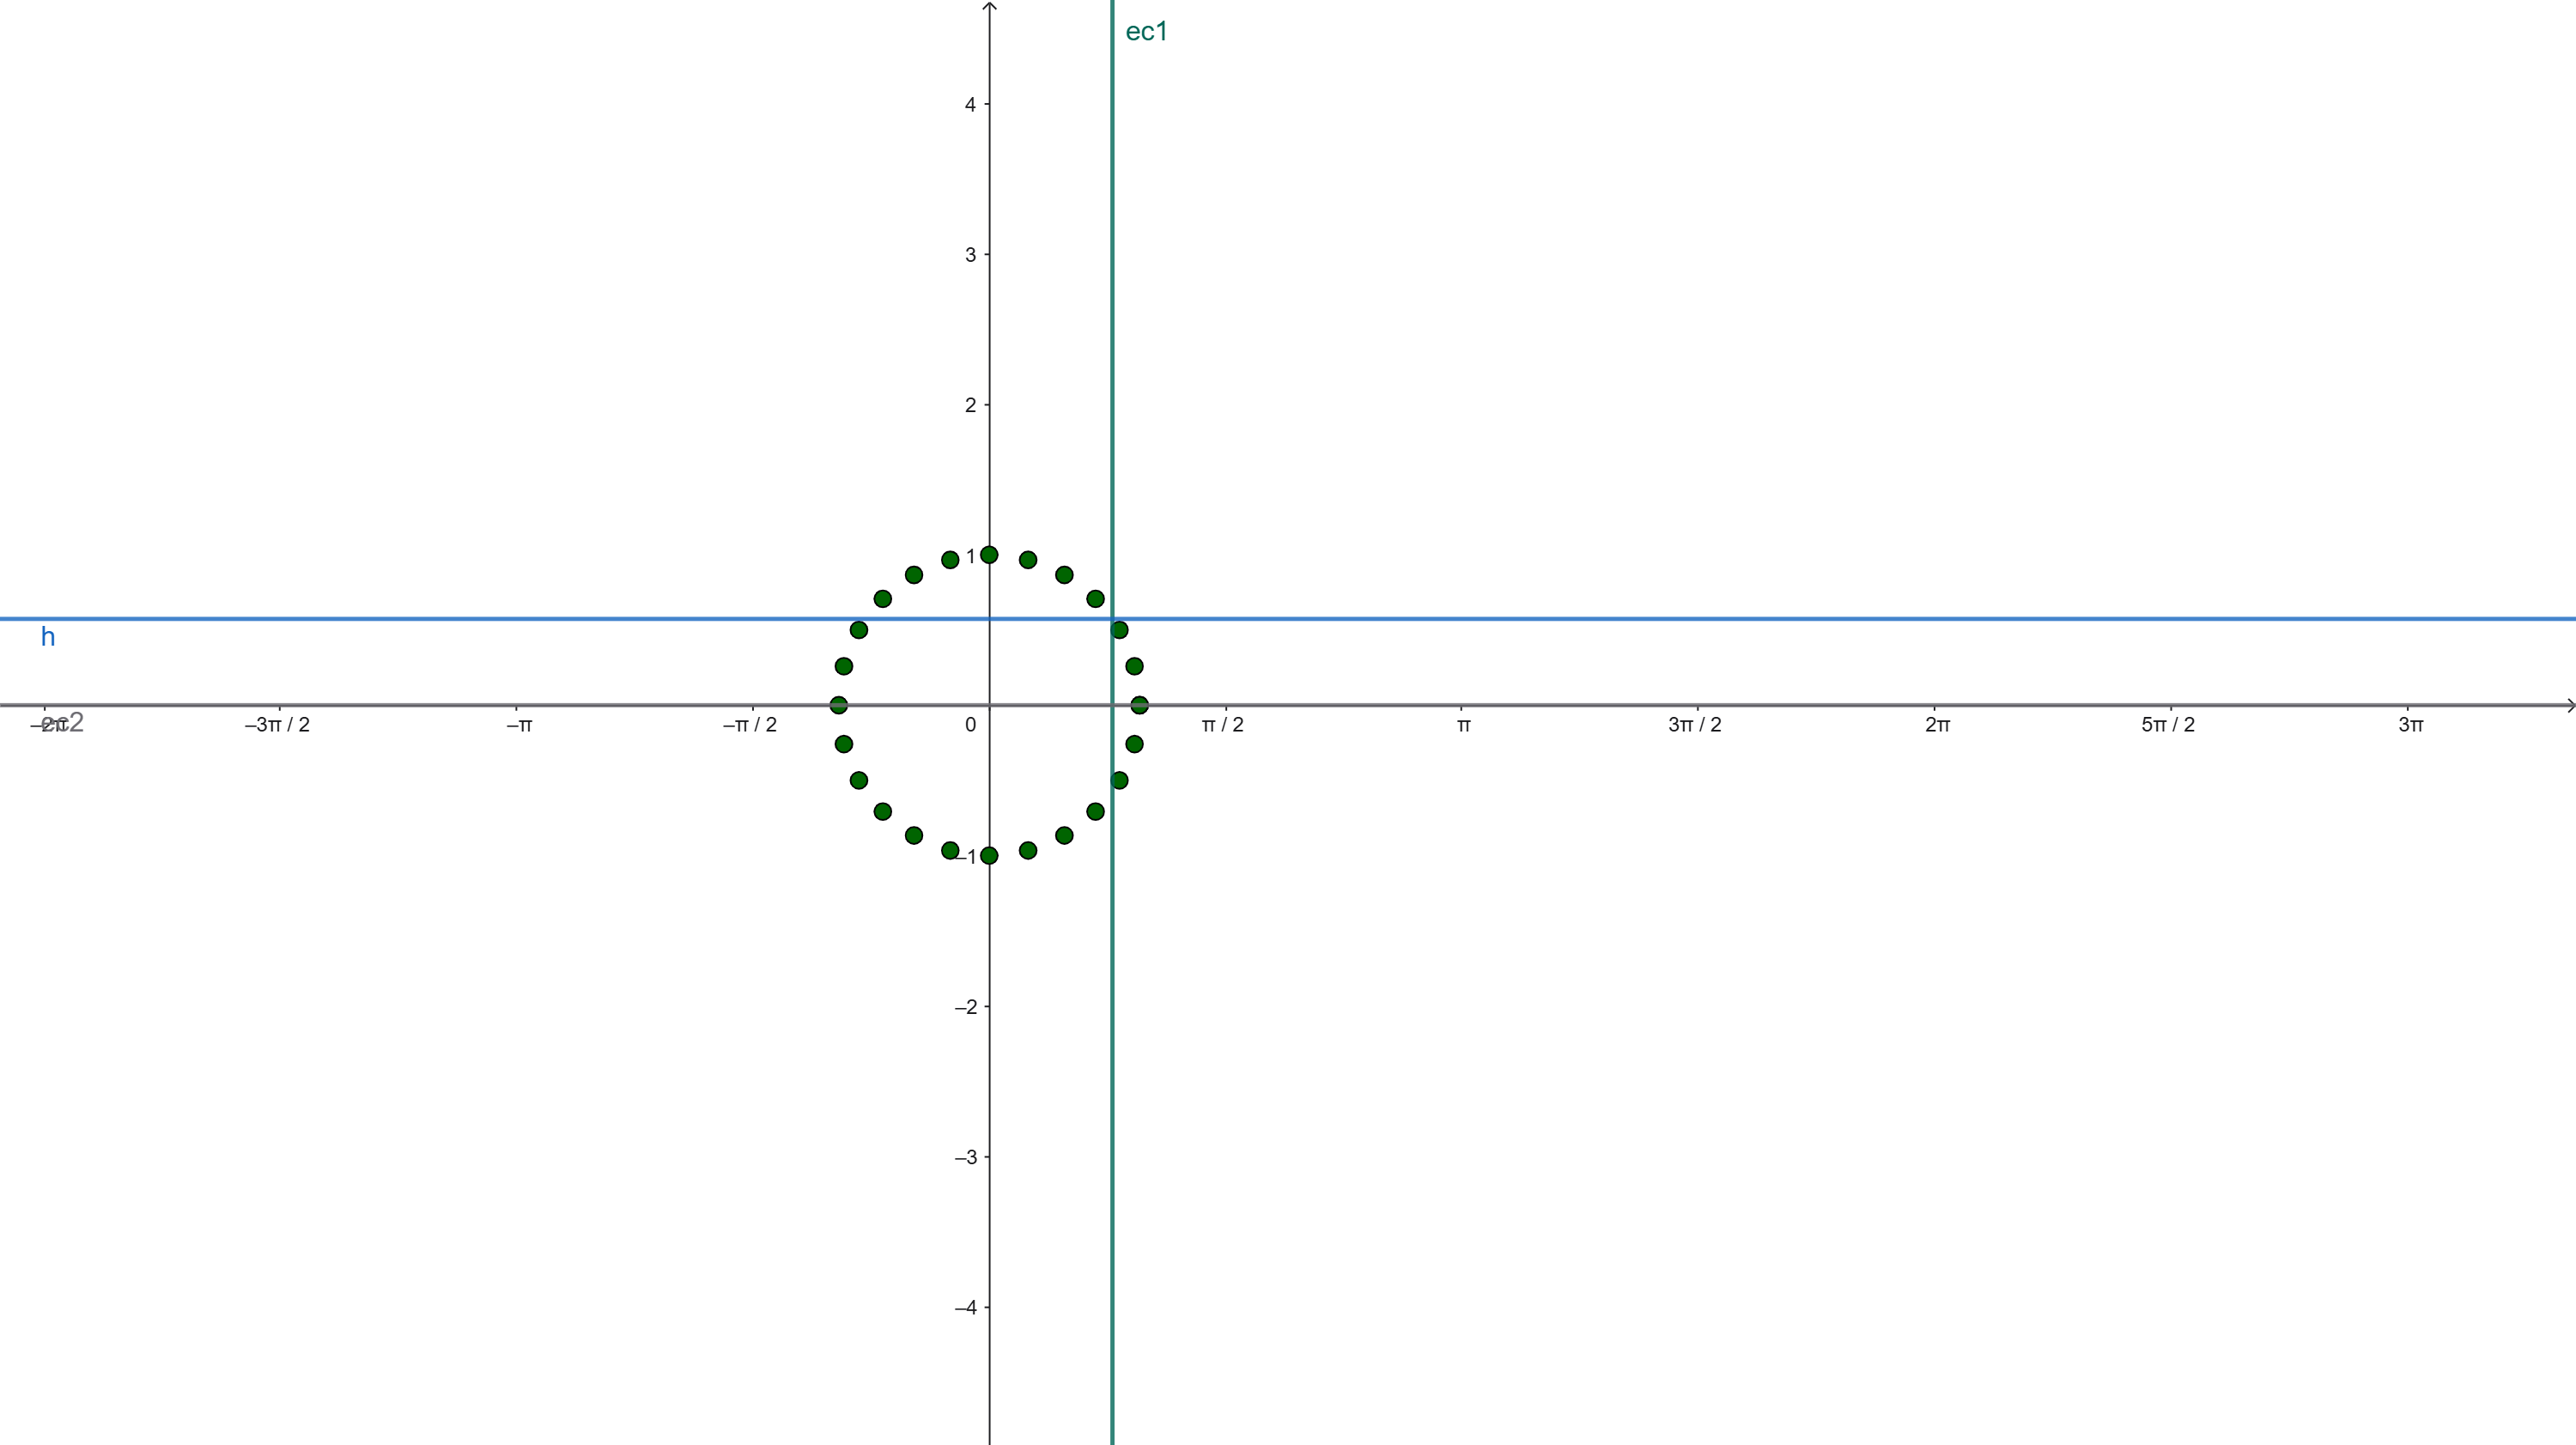
\includegraphics[width=0.55\textwidth]{Apendices/rc.png}
  \caption{Visualización discreta del comportamiento cíclico del tiempo} 
  \caption*{GeoGebra: Generación de puntos discretos sobre la circunferencia usando la expresión: \newline
  \texttt{Sequence((cos(2$\pi$ * n / 86400), sin(2$\pi$ * n / 86400)), n, 0, 86400, 3600)}}
  \caption*{La figura incluye dos líneas auxiliares que recorren la circunferencia: una horizontal (coseno) y una vertical (seno), generadas dinámicamente mediante un deslizador \( t \) con paso de 600 segundos. Estas líneas intersectan en el punto \( (x, y) \), representando la posición temporal proyectada en coordenadas trigonométricas.}
  \label{fig:representacion-ciclica-tiempo}
\end{figure}

\begin{figure}[ht!]
  \centering
  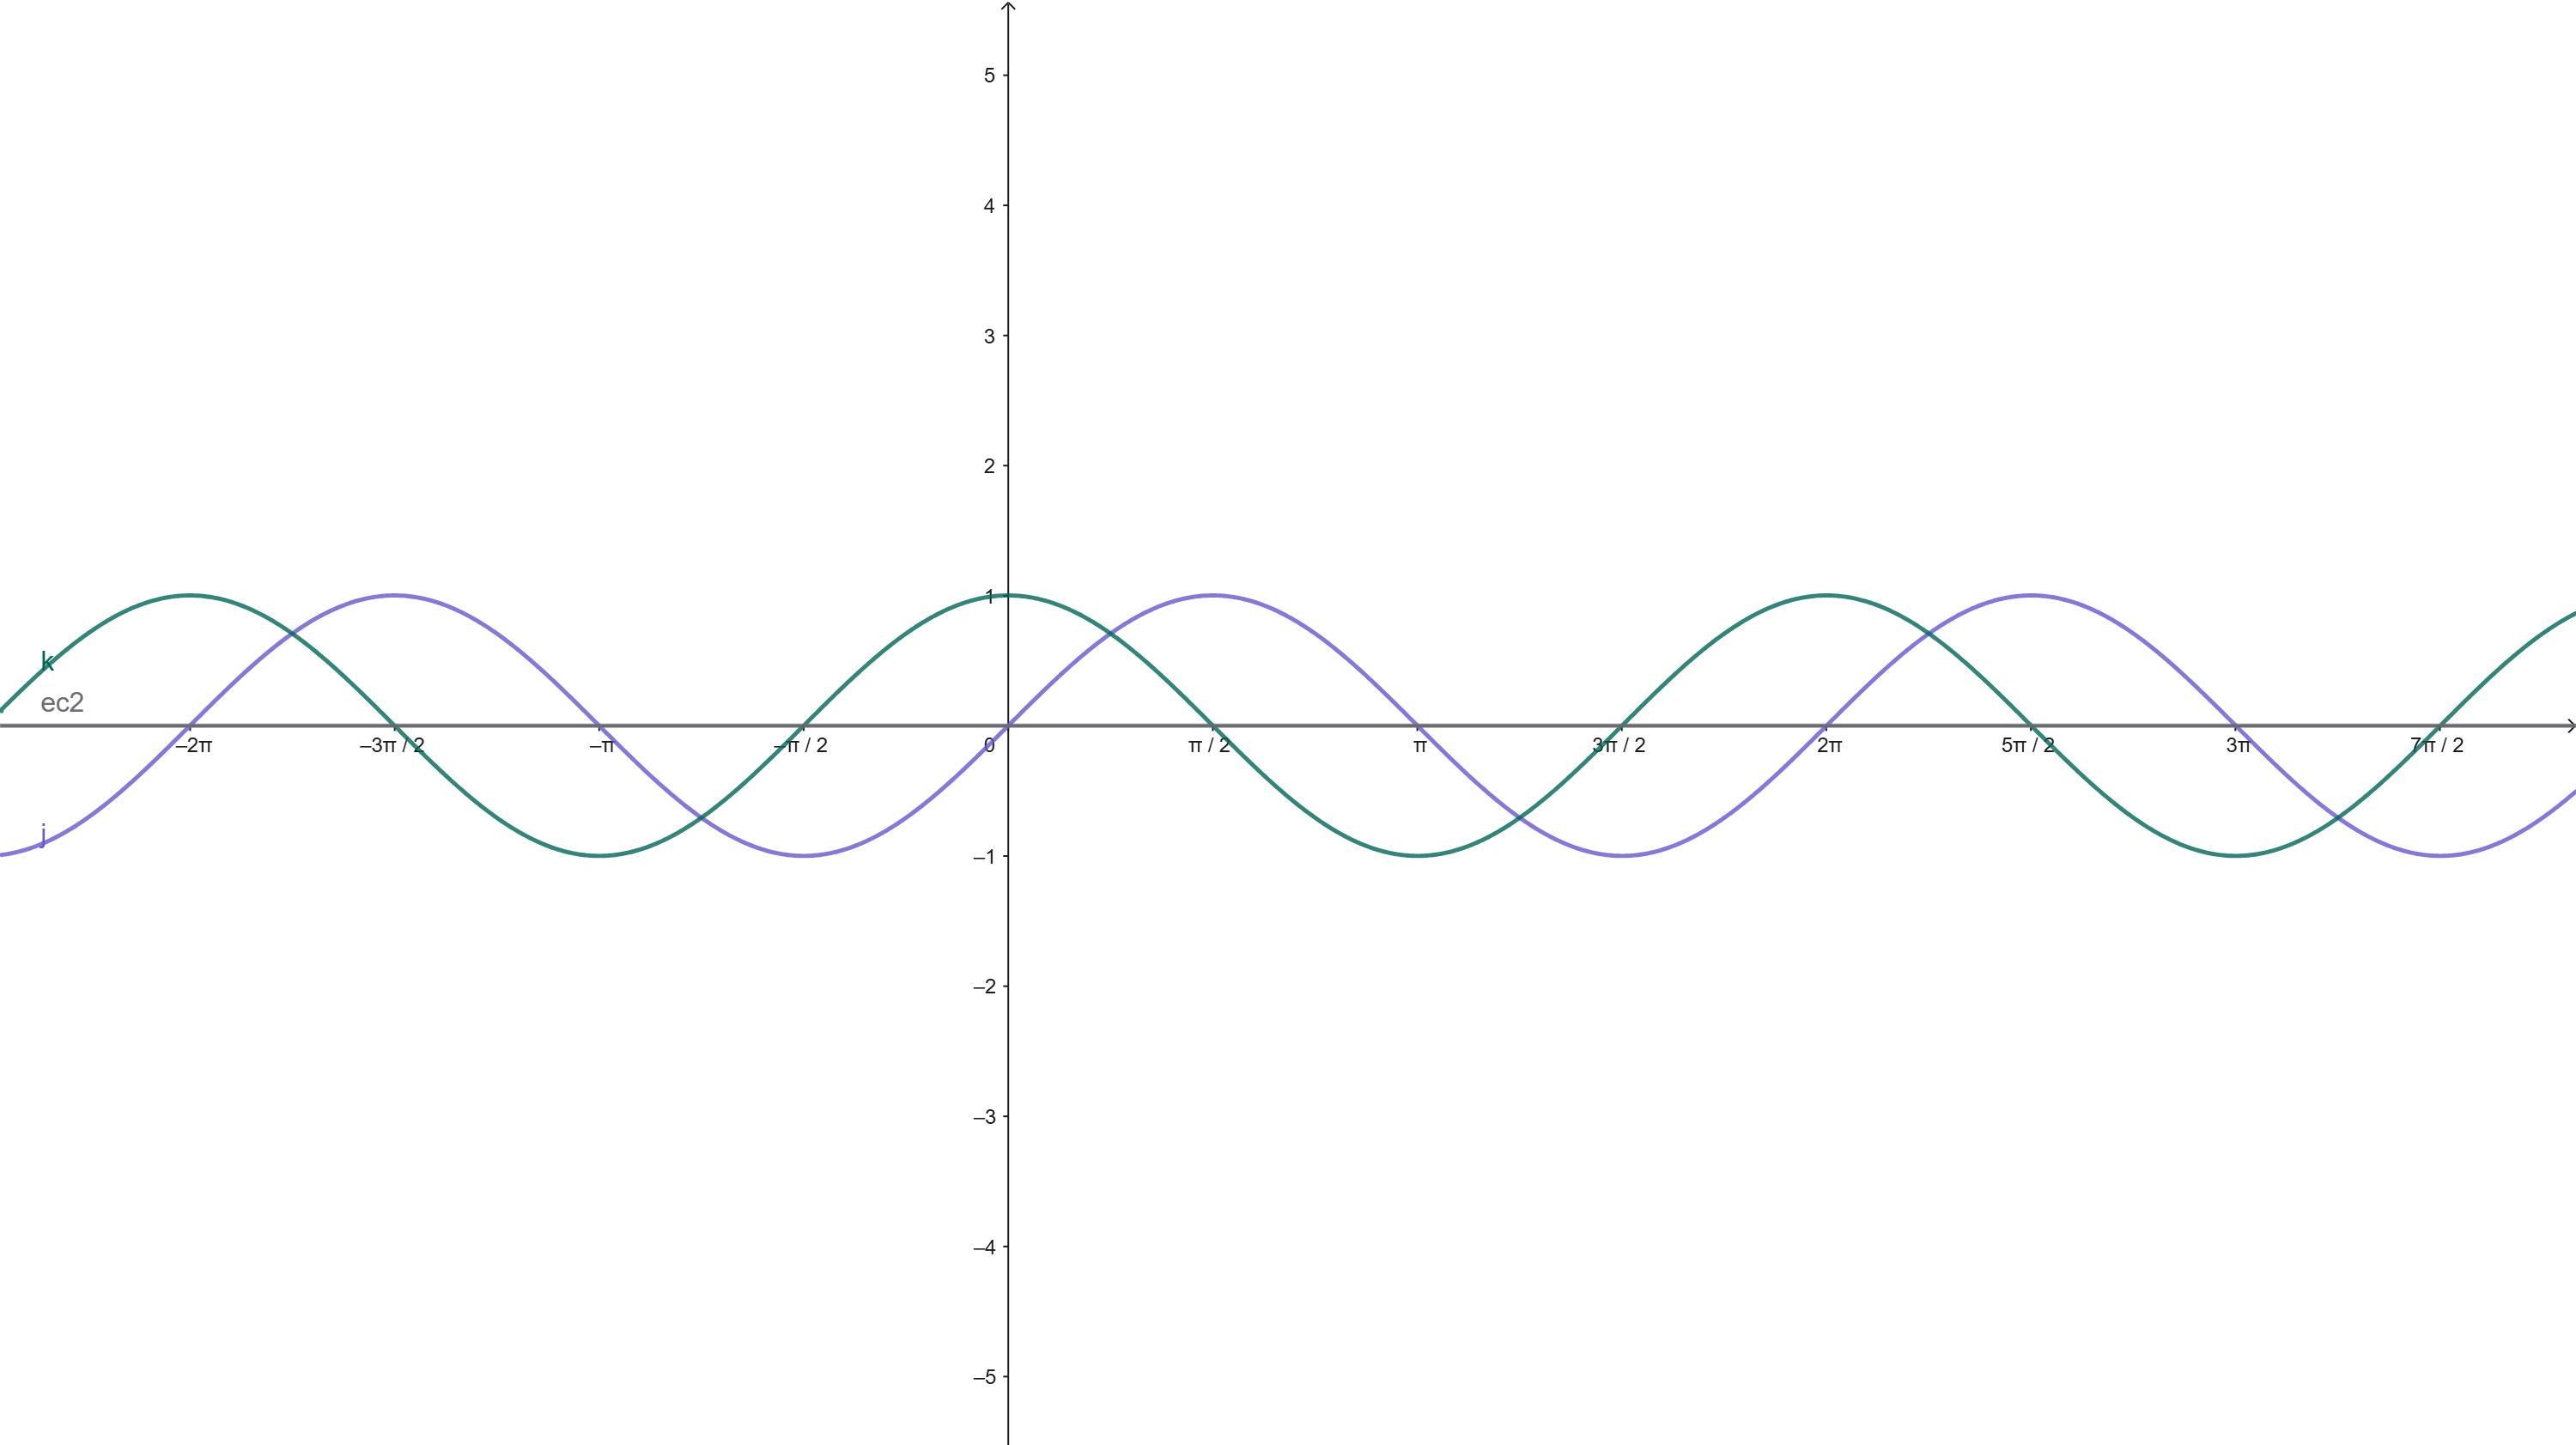
\includegraphics[width=0.55\textwidth]{Apendices/sencos.png}
  \caption{Visualización de las funciones seno y coseno  } 
  \caption*{GeoGebra: Generación de las funciones seno y coseno usando las expresiones: \newline
  \texttt{Sequence((x, sin(x)), x, 0, 2$\pi$, $\pi$/6)} y \newline
  \texttt{Sequence((x, cos(x)), x, 0, 2$\pi$, $\pi$/6)}}
  \label{fig: seno-coseno}
\end{figure}

\begin{figure}[ht!]
  \centering
  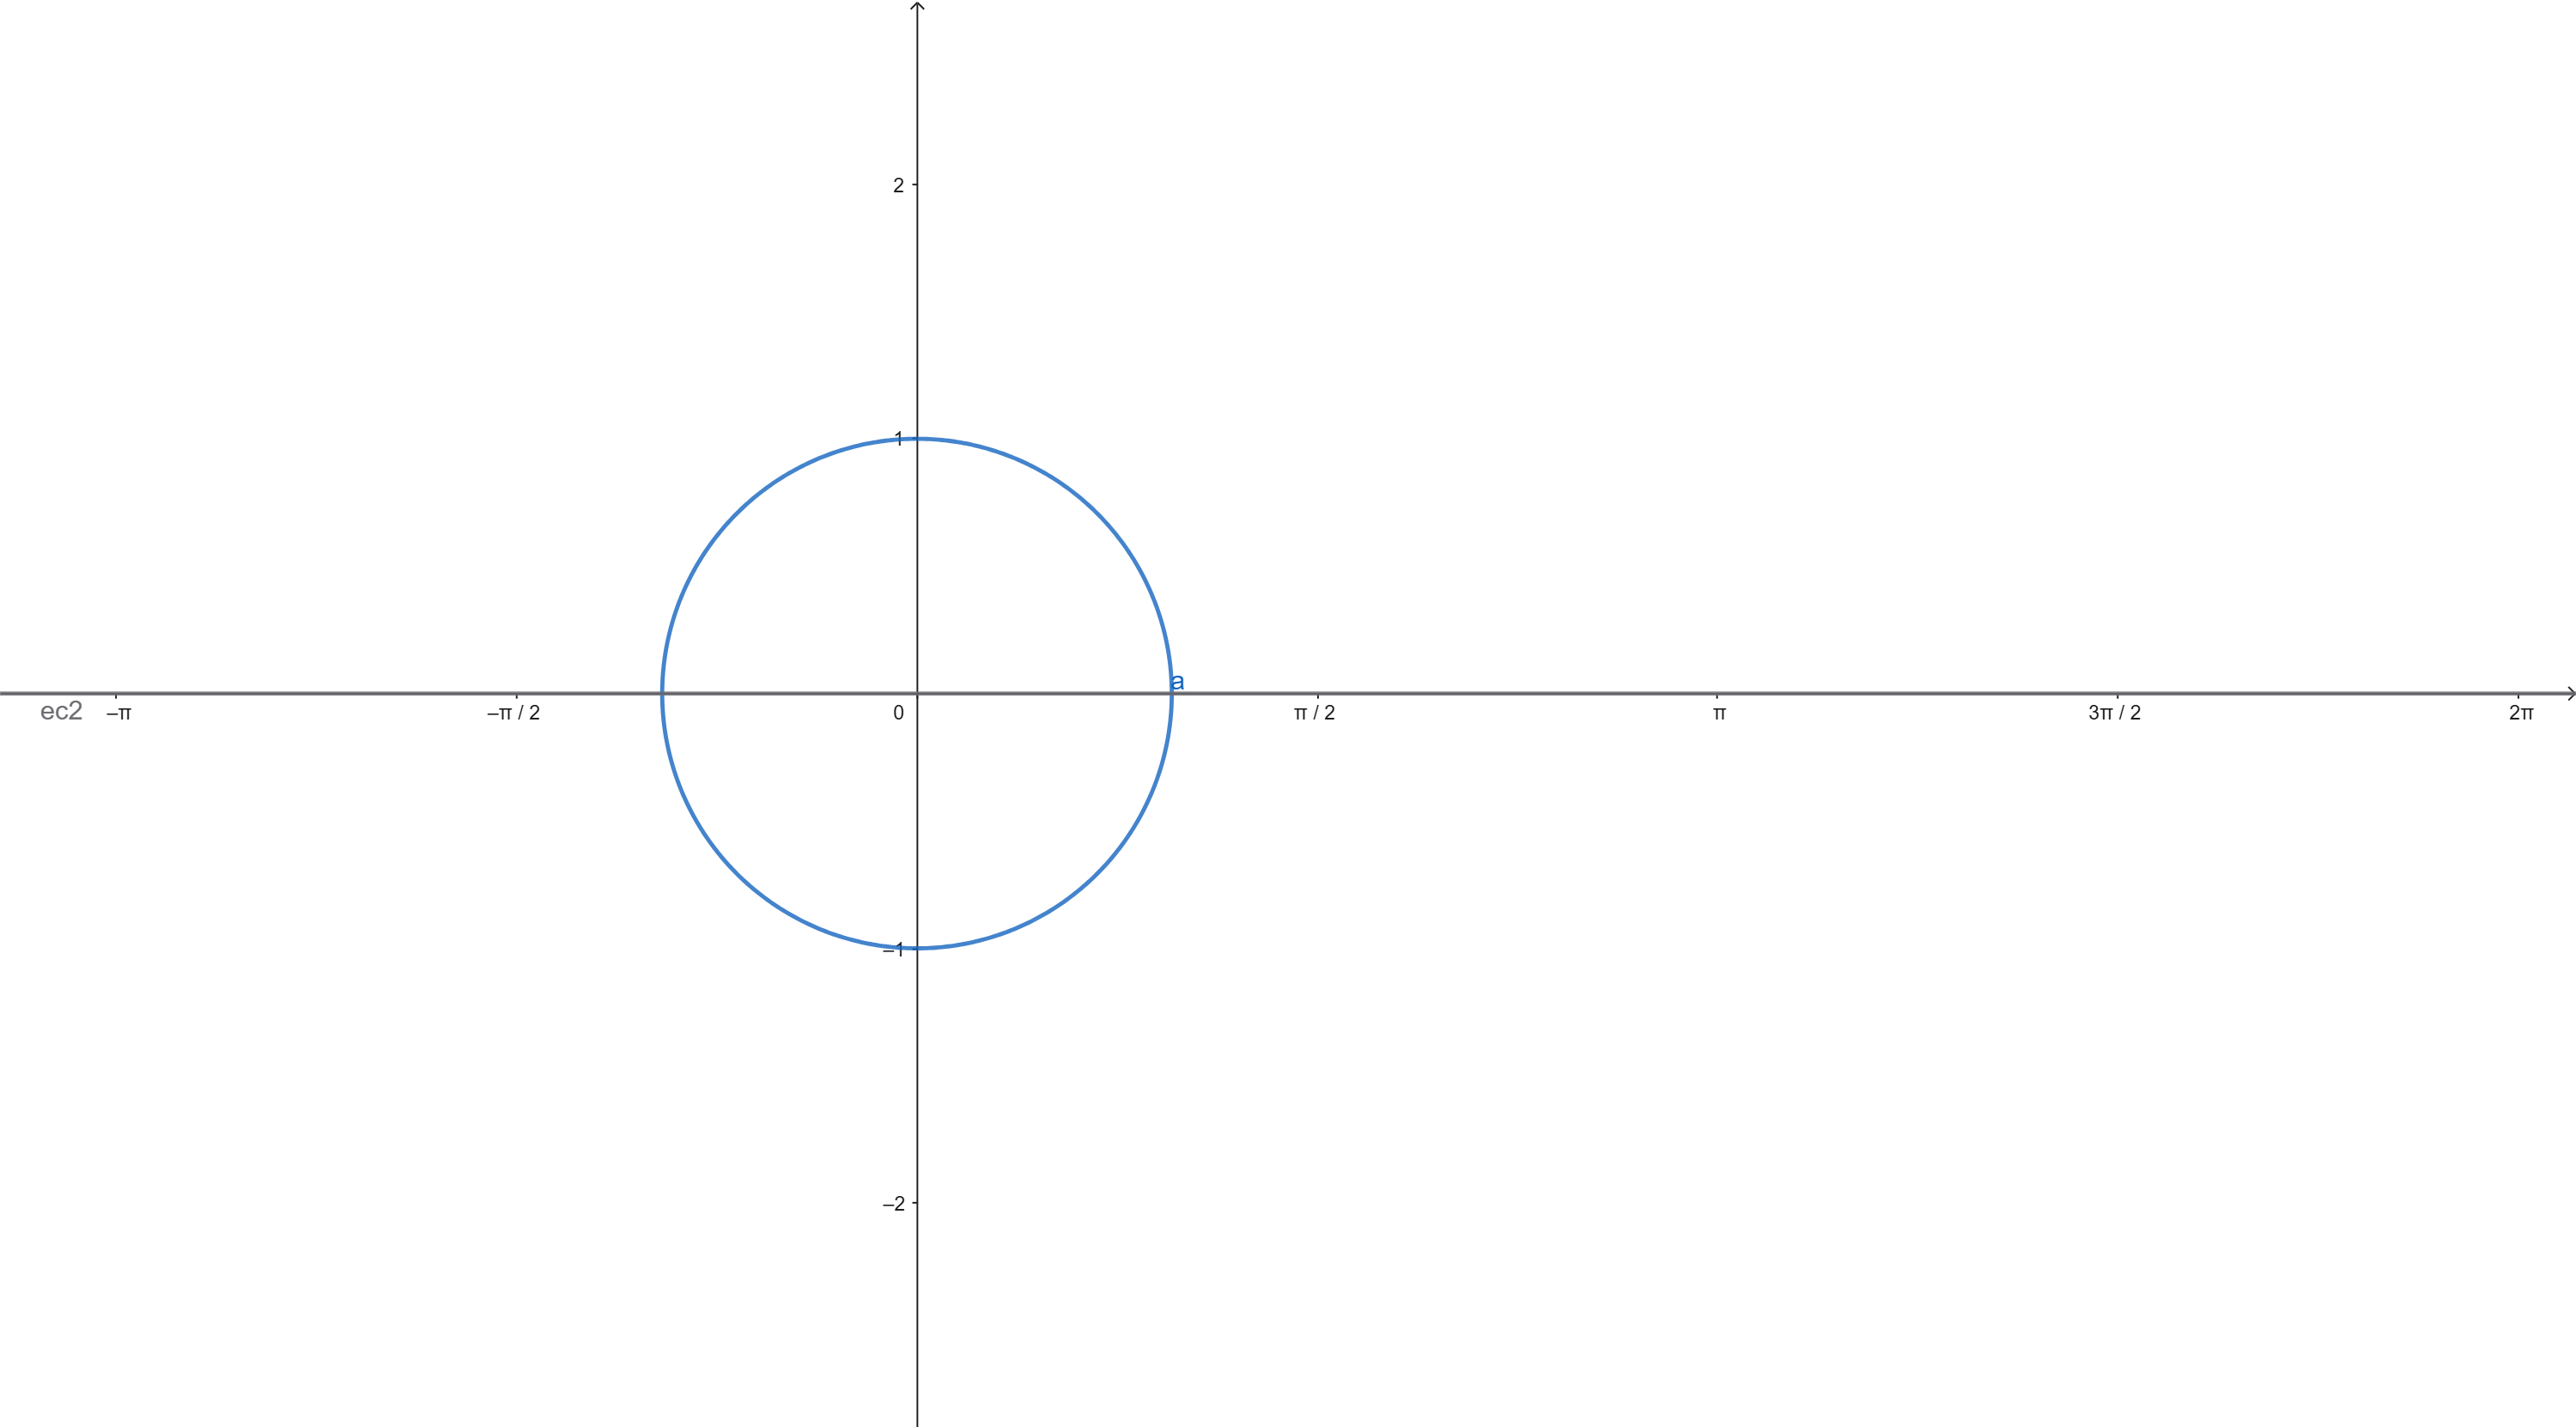
\includegraphics[width=0.55\textwidth]{Apendices/curve.png}
  \caption{Curva paramétrica continua del tiempo sobre el círculo unitario}
  \caption*{GeoGebra: Generación de la curva mediante las expresiones: \newline
  \texttt{x(t) = cos(2$\pi$ * t / 86400)}, \quad
  \texttt{y(t) = sin(2$\pi$ * t / 86400)}, \quad
  \texttt{Curve(x(t), y(t), t, 0, 86400)}}
  \caption*{La figura muestra una curva paramétrica continua que representa el tiempo sobre el círculo unitario mediante funciones trigonométricas. Cada instante se proyecta como un punto único definido por \( x(t) = \cos\left(\frac{2\pi t}{86400}\right) \) y \( y(t) = \sin\left(\frac{2\pi t}{86400}\right) \), donde \( t \) es el número de segundos desde las 00:00. Esta codificación garantiza continuidad angular, permitiendo que modelos de simulación o aprendizaje automático interpreten correctamente la naturaleza cíclica del tiempo sin ambigüedades en los extremos del día.}
  \label{fig:curva-tiempo-circular}
\end{figure}
\uextra{Apendice}{Verificación del sistema de monitoreo acústico}

{\small
  \begin{longtable}[c]{c p{3.5cm} p{2.2cm} p{2.2cm} p{3.5cm}}
    \hline
    \textbf{Requerimiento} & \textbf{Descripción}                                                                                    & \textbf{Entrada}                                                  & \textbf{Salida}                                                       & \textbf{Criterio de Aceptación}                                                       \\
    \hline
    \endfirsthead

    \hline
    \textbf{Requerimiento} & \textbf{Descripción}                                                                                    & \textbf{Entrada}                                                  & \textbf{Salida}                                                       & \textbf{Criterio de Aceptación}                                                       \\
    \hline
    \endhead
    \endfoot
    \endlastfoot

    R1                     & Captura continua del audio ambiental a través de micrófonos.                                            & Señales de audio del entorno a través del hardware del micrófono. & Eventos discretos etiquedados del audio.                              & El sistema debe estar activo y registrando datos en todo momento.                     \\
    \addlinespace
    R2                     & Procesamiento del audio para clasificarlo en eventos sonoros predefinidos.                              & Flujo de datos de audio.                                          & Clasificación del sonido (ej. voz, silencio, golpe).                  & El sistema debe etiquetar correctamente la señal de audio que recibe en todo momento. \\
    \addlinespace
    R3                     & El sistema debe conocer en todo momento el estado de actividad del entorno.                             & Señal de audio.                                                   & Hay ruido o silencio.                                                 & El sistema reconoce cuando hay ruido o silencio.                                      \\
    \addlinespace
    R4                     & Comparación de la actividad en tiempo real con el perfil de normalidad para detectar patrones anómalos. & Secuencia de eventos en tiempo real                               & Identificación de una anomalía o evento atípico.                      & Detectar si una secuencia de eventos es normal o anómala.                             \\
    \addlinespace
    R5                     & El sistema realiza una consulta verbal al usuario al detectar una anomalía.                             & Señal de audio.                                                   & Emisión de una pregunta de voz pregrabada (ej. ``¿Está todo bien?''). & El sistema consulta el estado del usuario antes de enviar una alerta.                 \\
    \addlinespace
    R6                     & Permitir cancelar una alerta de emergencia por comando de voz.                                          & Respuesta de voz del usuario (ej. ``Estoy bien'').                & No se envía alerta.                                                   & El sistema cancela la alerta.                                                         \\
    \addlinespace
    R7                     & El sistema envía notificaciones de emergencia si la anomalía es crítica o el usuario no responde.       & Falta de respuesta del usuario o gravedad de la anomalía          & Envío de notificaciones.                                              & El sistema es capaz de enviar una alerta sin la intervención del usuario.             \\
    \bottomrule
    \addlinespace

    \caption{Requerimientos del sistema acústico}
    \label{tab:requerimientos_sistema_acustico}
  \end{longtable}
}

\titleformat{\chapter}
{\normalfont\fontsize{12}{15}\centering}{Anexos \thechapter.}{0.3em}{}[]

\clearpage
\thispagestyle{empty}
\begin{center}
  \vspace*{\fill}
  \phantomsection
  Apéndices
  \addcontentsline{toc}{chapter}{Anexos}
  \vspace*{\fill}
\end{center}
\clearpage

\appendix
% \uextra{Apendice}{Dispositivo Raspberry Pi 4 Model B}
% \begin{figure}[ht!]
%   \centering
%   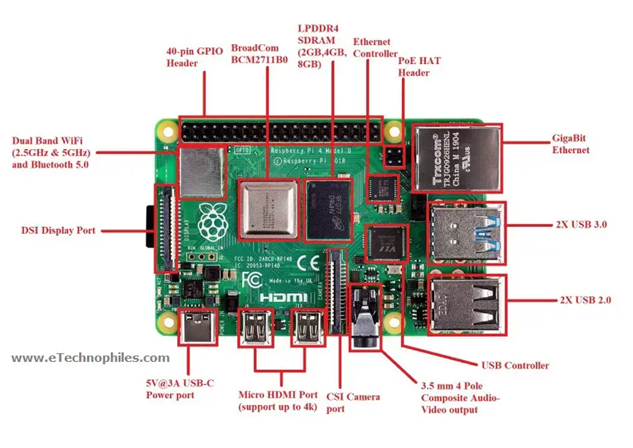
\includegraphics[width=0.95\textwidth]{Anexos/1.arquitectura-raspberry.png}
%   \caption{Arquitectura del Raspberry Pi 4 Model B}
%   \label{fig:raspberry-architecture}
% \end{figure}

\uextra{Apendice}{Representación cíclica del tiempo mediante funciones trigonométricas}
\begin{figure}[ht!]
  \centering
  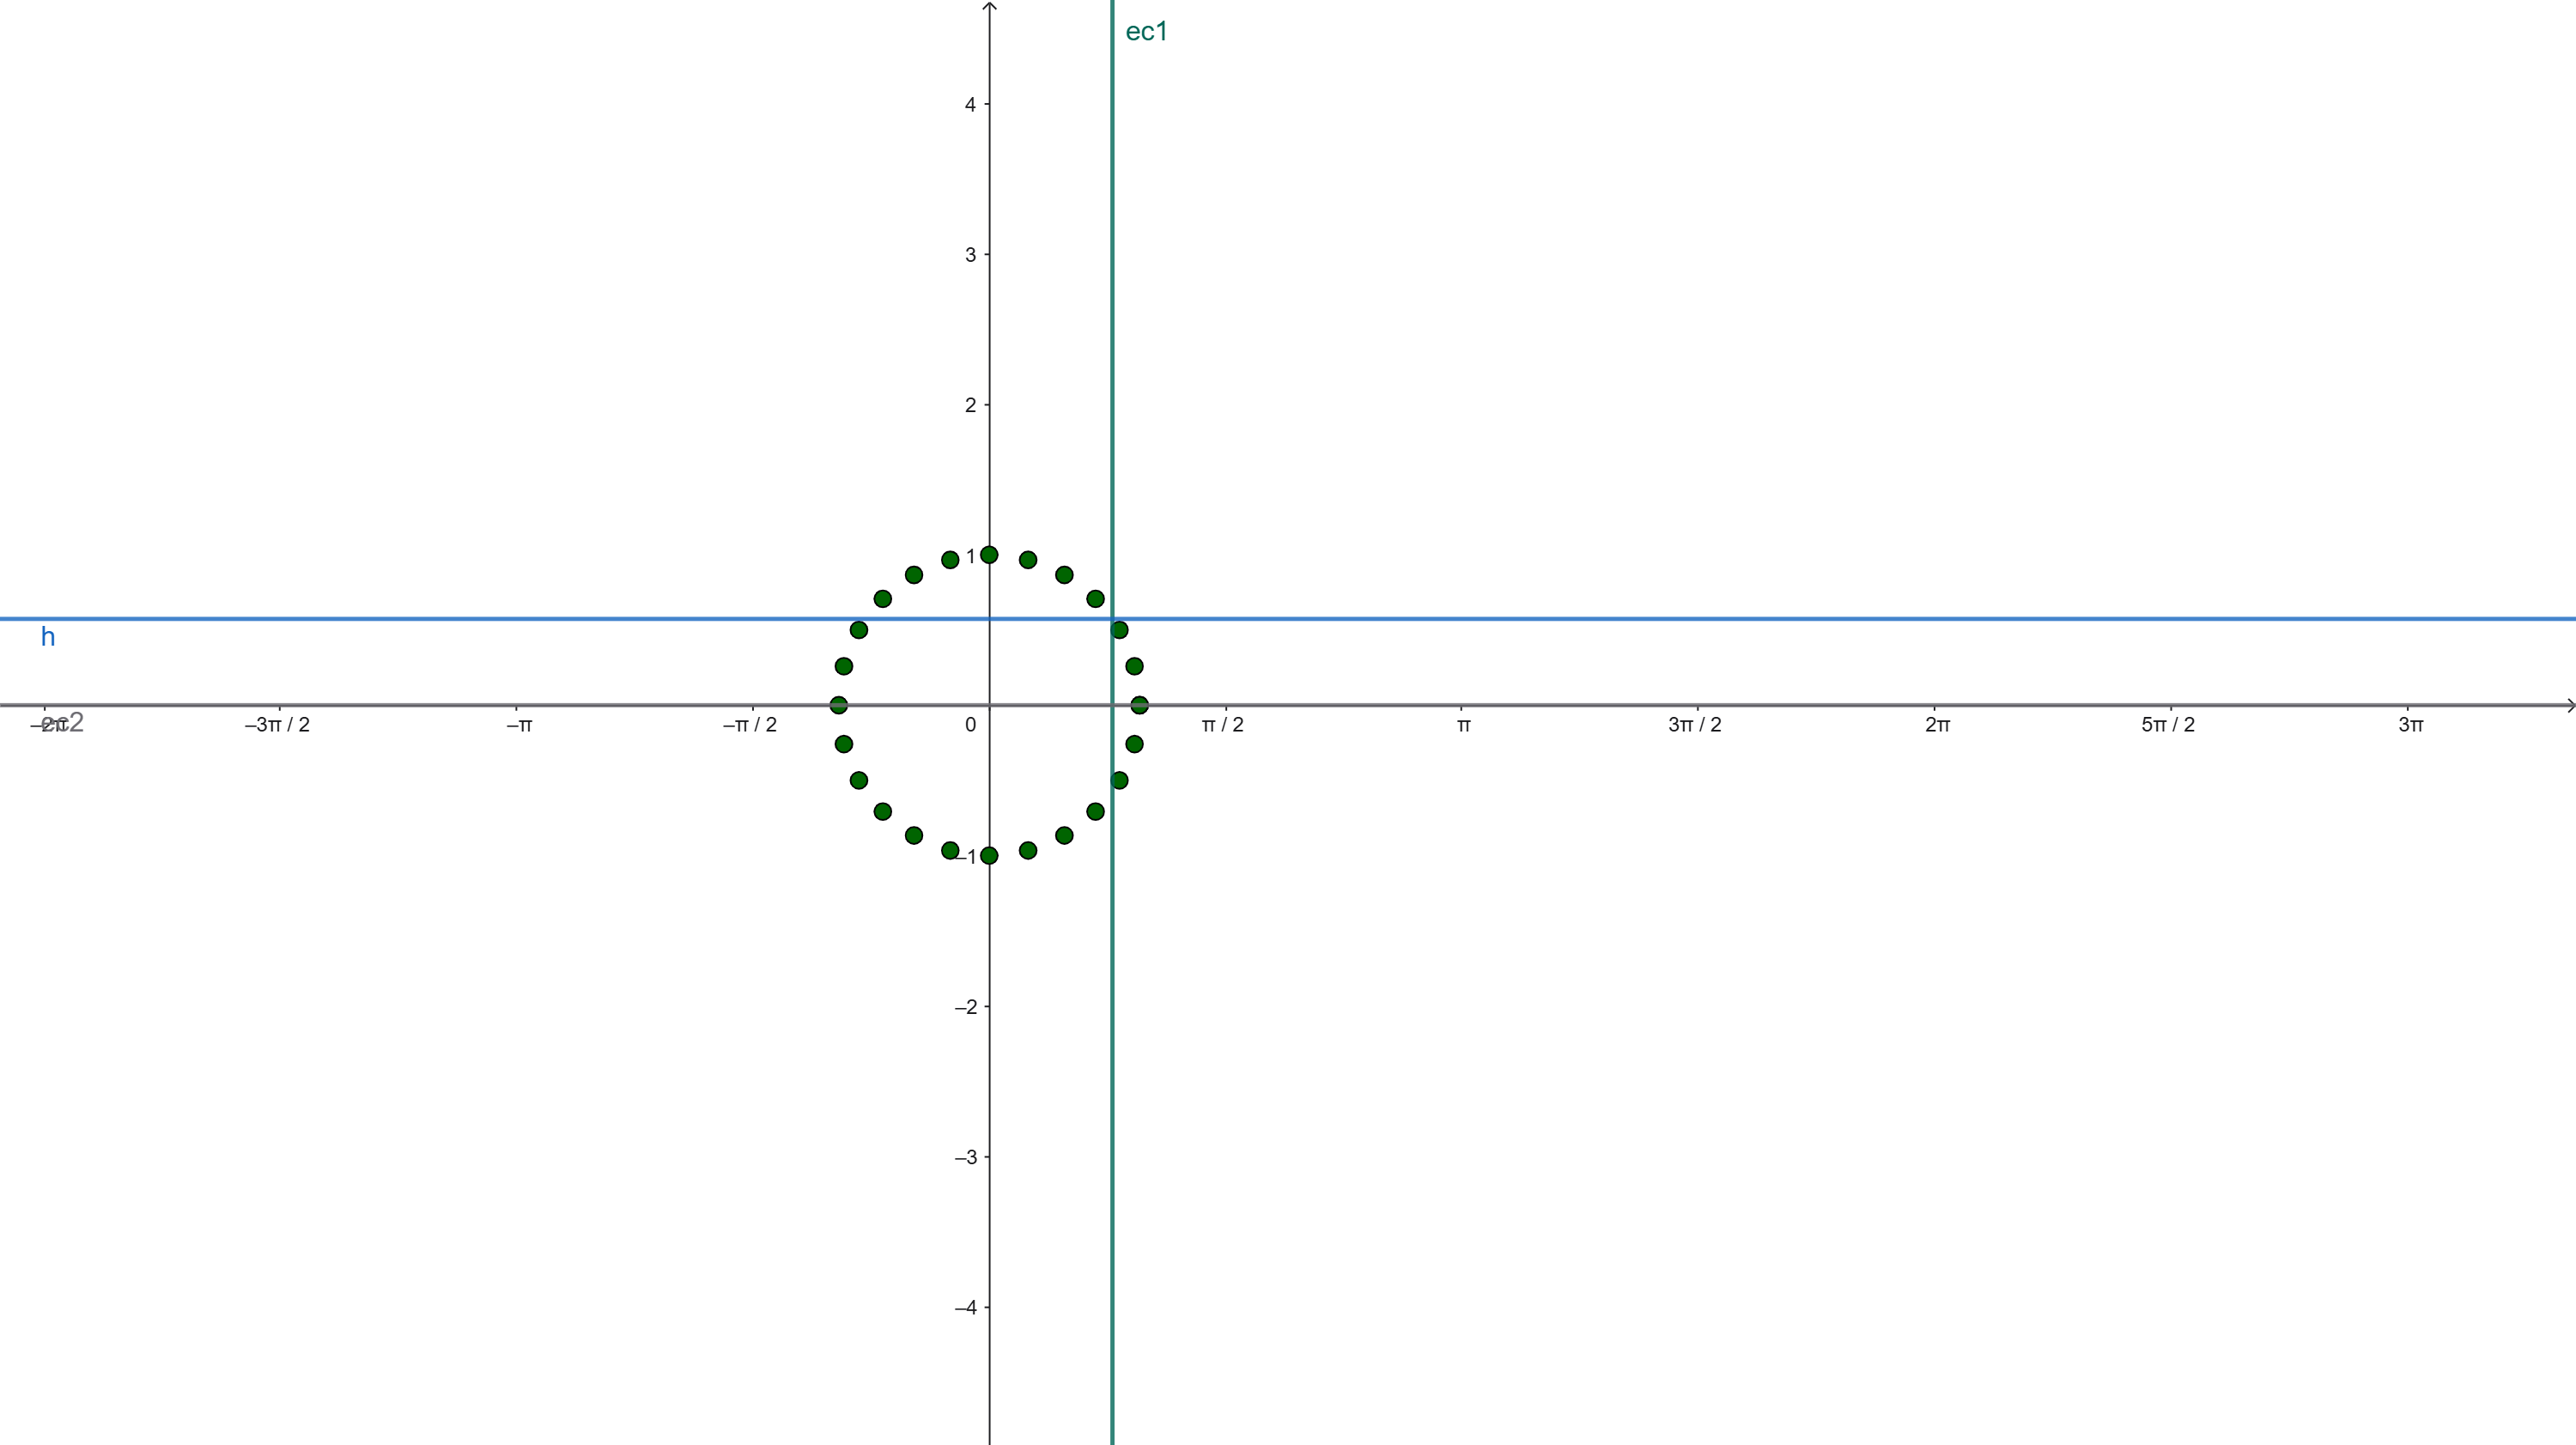
\includegraphics[width=0.55\textwidth]{Apendices/rc.png}
  \caption{Visualización discreta del comportamiento cíclico del tiempo} 
  \caption*{GeoGebra: Generación de puntos discretos sobre la circunferencia usando la expresión: \newline
  \texttt{Sequence((cos(2$\pi$ * n / 86400), sin(2$\pi$ * n / 86400)), n, 0, 86400, 3600)}}
  \caption*{La figura incluye dos líneas auxiliares que recorren la circunferencia: una horizontal (coseno) y una vertical (seno), generadas dinámicamente mediante un deslizador \( t \) con paso de 600 segundos. Estas líneas intersectan en el punto \( (x, y) \), representando la posición temporal proyectada en coordenadas trigonométricas.}
  \label{fig:representacion-ciclica-tiempo}
\end{figure}

\begin{figure}[ht!]
  \centering
  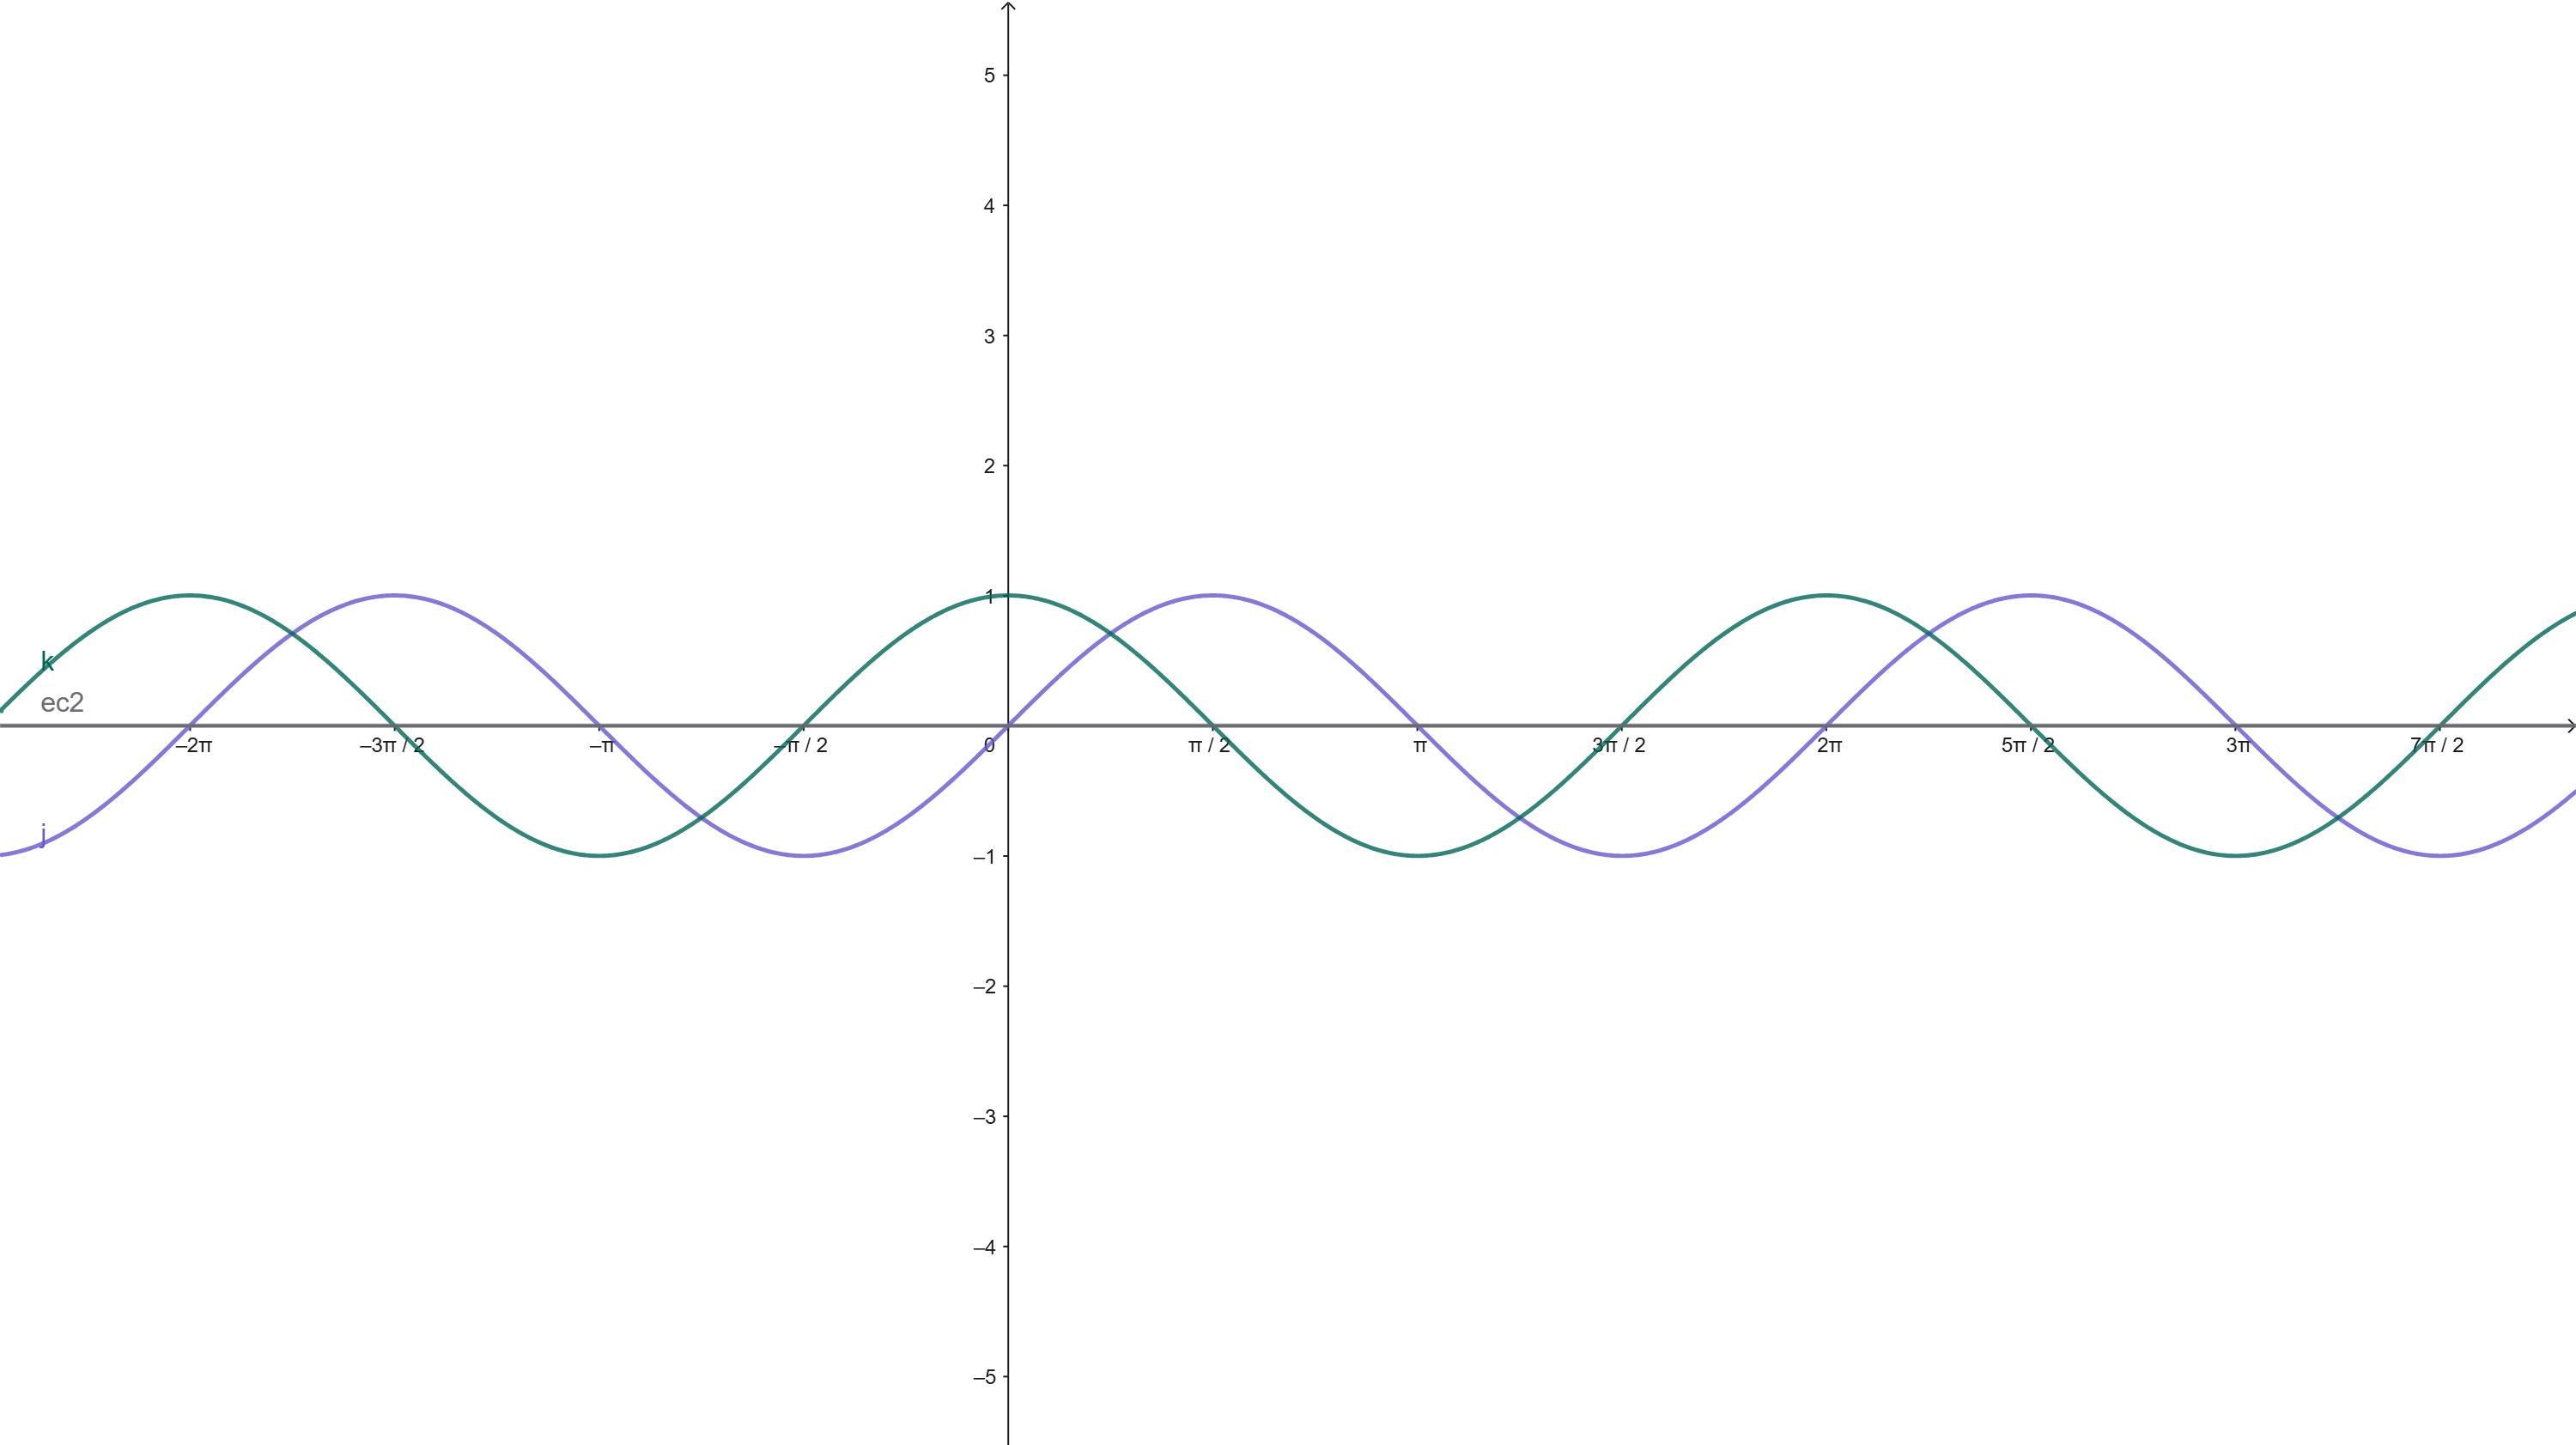
\includegraphics[width=0.55\textwidth]{Apendices/sencos.png}
  \caption{Visualización de las funciones seno y coseno  } 
  \caption*{GeoGebra: Generación de las funciones seno y coseno usando las expresiones: \newline
  \texttt{Sequence((x, sin(x)), x, 0, 2$\pi$, $\pi$/6)} y \newline
  \texttt{Sequence((x, cos(x)), x, 0, 2$\pi$, $\pi$/6)}}
  \label{fig: seno-coseno}
\end{figure}

\begin{figure}[ht!]
  \centering
  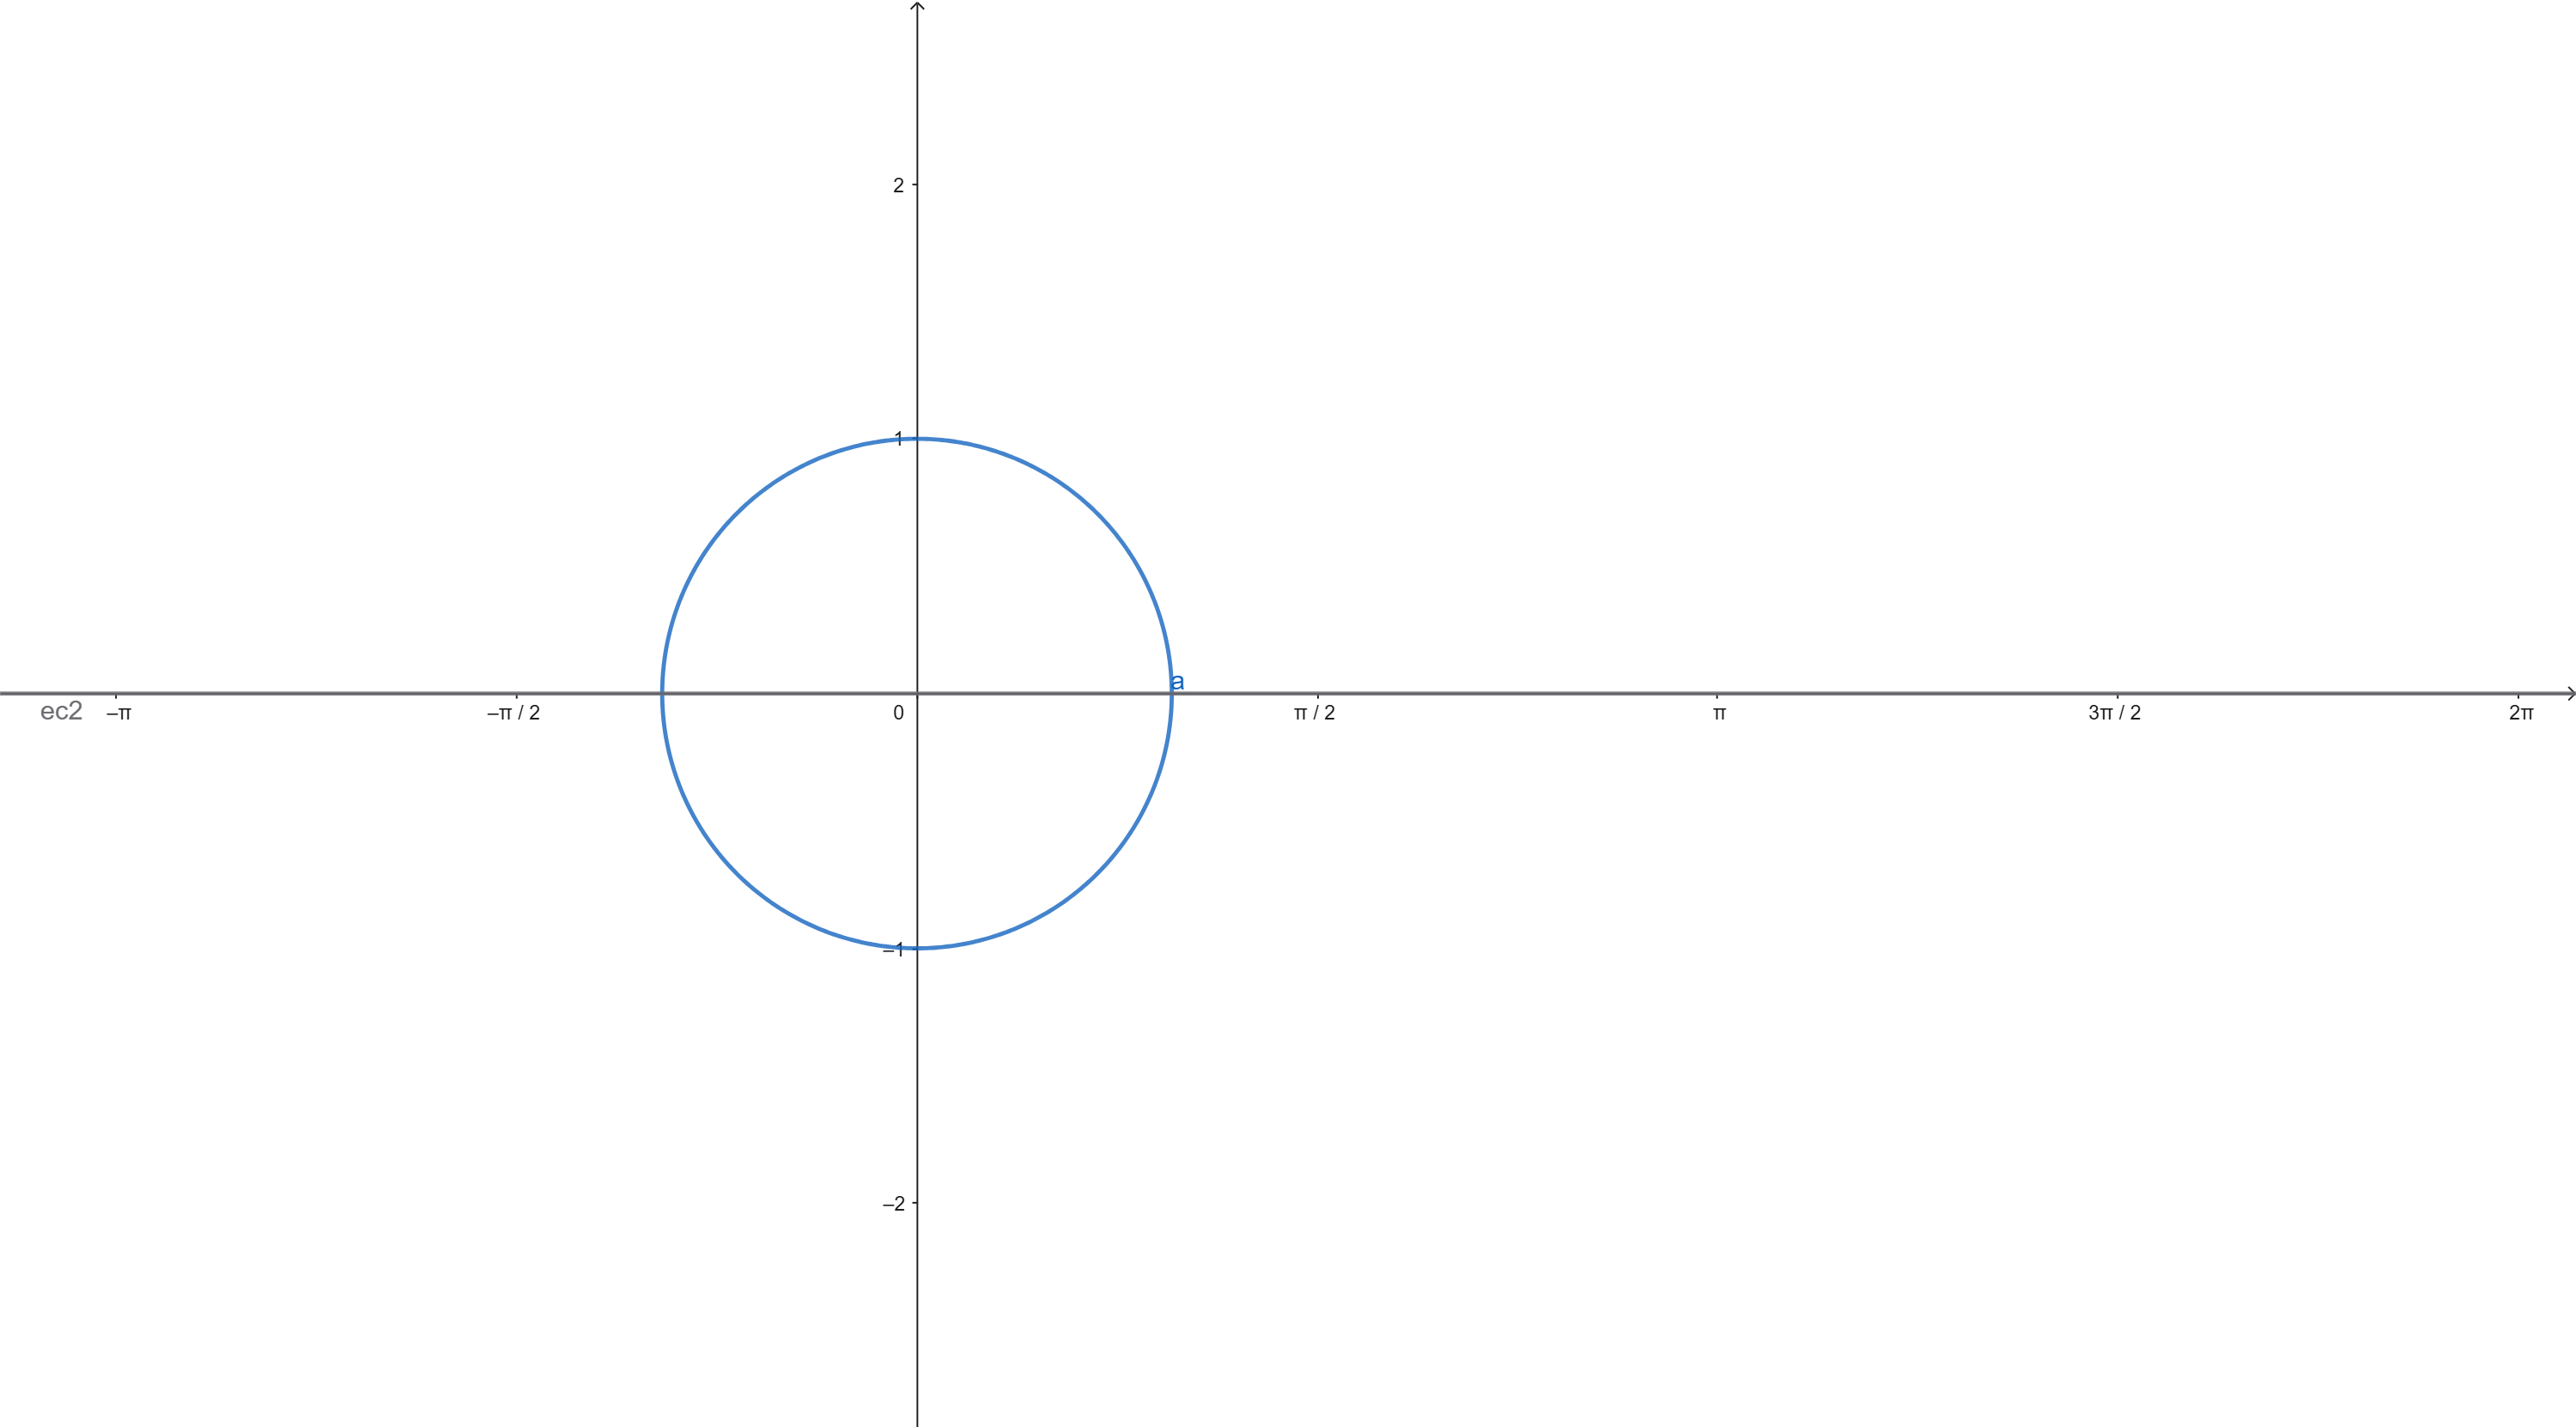
\includegraphics[width=0.55\textwidth]{Apendices/curve.png}
  \caption{Curva paramétrica continua del tiempo sobre el círculo unitario}
  \caption*{GeoGebra: Generación de la curva mediante las expresiones: \newline
  \texttt{x(t) = cos(2$\pi$ * t / 86400)}, \quad
  \texttt{y(t) = sin(2$\pi$ * t / 86400)}, \quad
  \texttt{Curve(x(t), y(t), t, 0, 86400)}}
  \caption*{La figura muestra una curva paramétrica continua que representa el tiempo sobre el círculo unitario mediante funciones trigonométricas. Cada instante se proyecta como un punto único definido por \( x(t) = \cos\left(\frac{2\pi t}{86400}\right) \) y \( y(t) = \sin\left(\frac{2\pi t}{86400}\right) \), donde \( t \) es el número de segundos desde las 00:00. Esta codificación garantiza continuidad angular, permitiendo que modelos de simulación o aprendizaje automático interpreten correctamente la naturaleza cíclica del tiempo sin ambigüedades en los extremos del día.}
  \label{fig:curva-tiempo-circular}
\end{figure}
\uextra{Apendice}{Verificación del sistema de monitoreo acústico}

{\small
  \begin{longtable}[c]{c p{3.5cm} p{2.2cm} p{2.2cm} p{3.5cm}}
    \hline
    \textbf{Requerimiento} & \textbf{Descripción}                                                                                    & \textbf{Entrada}                                                  & \textbf{Salida}                                                       & \textbf{Criterio de Aceptación}                                                       \\
    \hline
    \endfirsthead

    \hline
    \textbf{Requerimiento} & \textbf{Descripción}                                                                                    & \textbf{Entrada}                                                  & \textbf{Salida}                                                       & \textbf{Criterio de Aceptación}                                                       \\
    \hline
    \endhead
    \endfoot
    \endlastfoot

    R1                     & Captura continua del audio ambiental a través de micrófonos.                                            & Señales de audio del entorno a través del hardware del micrófono. & Eventos discretos etiquedados del audio.                              & El sistema debe estar activo y registrando datos en todo momento.                     \\
    \addlinespace
    R2                     & Procesamiento del audio para clasificarlo en eventos sonoros predefinidos.                              & Flujo de datos de audio.                                          & Clasificación del sonido (ej. voz, silencio, golpe).                  & El sistema debe etiquetar correctamente la señal de audio que recibe en todo momento. \\
    \addlinespace
    R3                     & El sistema debe conocer en todo momento el estado de actividad del entorno.                             & Señal de audio.                                                   & Hay ruido o silencio.                                                 & El sistema reconoce cuando hay ruido o silencio.                                      \\
    \addlinespace
    R4                     & Comparación de la actividad en tiempo real con el perfil de normalidad para detectar patrones anómalos. & Secuencia de eventos en tiempo real                               & Identificación de una anomalía o evento atípico.                      & Detectar si una secuencia de eventos es normal o anómala.                             \\
    \addlinespace
    R5                     & El sistema realiza una consulta verbal al usuario al detectar una anomalía.                             & Señal de audio.                                                   & Emisión de una pregunta de voz pregrabada (ej. ``¿Está todo bien?''). & El sistema consulta el estado del usuario antes de enviar una alerta.                 \\
    \addlinespace
    R6                     & Permitir cancelar una alerta de emergencia por comando de voz.                                          & Respuesta de voz del usuario (ej. ``Estoy bien'').                & No se envía alerta.                                                   & El sistema cancela la alerta.                                                         \\
    \addlinespace
    R7                     & El sistema envía notificaciones de emergencia si la anomalía es crítica o el usuario no responde.       & Falta de respuesta del usuario o gravedad de la anomalía          & Envío de notificaciones.                                              & El sistema es capaz de enviar una alerta sin la intervención del usuario.             \\
    \bottomrule
    \addlinespace

    \caption{Requerimientos del sistema acústico}
    \label{tab:requerimientos_sistema_acustico}
  \end{longtable}
}

\titleformat{\chapter}
{\normalfont\fontsize{12}{15}\centering}{Anexos \thechapter.}{0.3em}{}[]

\clearpage
\thispagestyle{empty}
\begin{center}
  \vspace*{\fill}
  \phantomsection
  Apéndices
  \addcontentsline{toc}{chapter}{Anexos}
  \vspace*{\fill}
\end{center}
\clearpage

\appendix
% \uextra{Apendice}{Dispositivo Raspberry Pi 4 Model B}
% \begin{figure}[ht!]
%   \centering
%   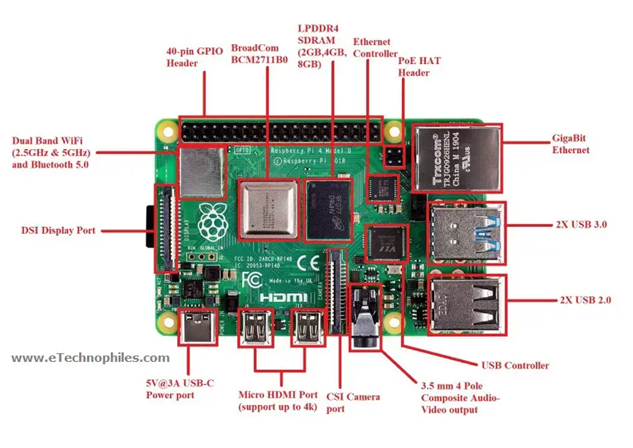
\includegraphics[width=0.95\textwidth]{Anexos/1.arquitectura-raspberry.png}
%   \caption{Arquitectura del Raspberry Pi 4 Model B}
%   \label{fig:raspberry-architecture}
% \end{figure}

\uextra{Apendice}{Representación cíclica del tiempo mediante funciones trigonométricas}
\begin{figure}[ht!]
  \centering
  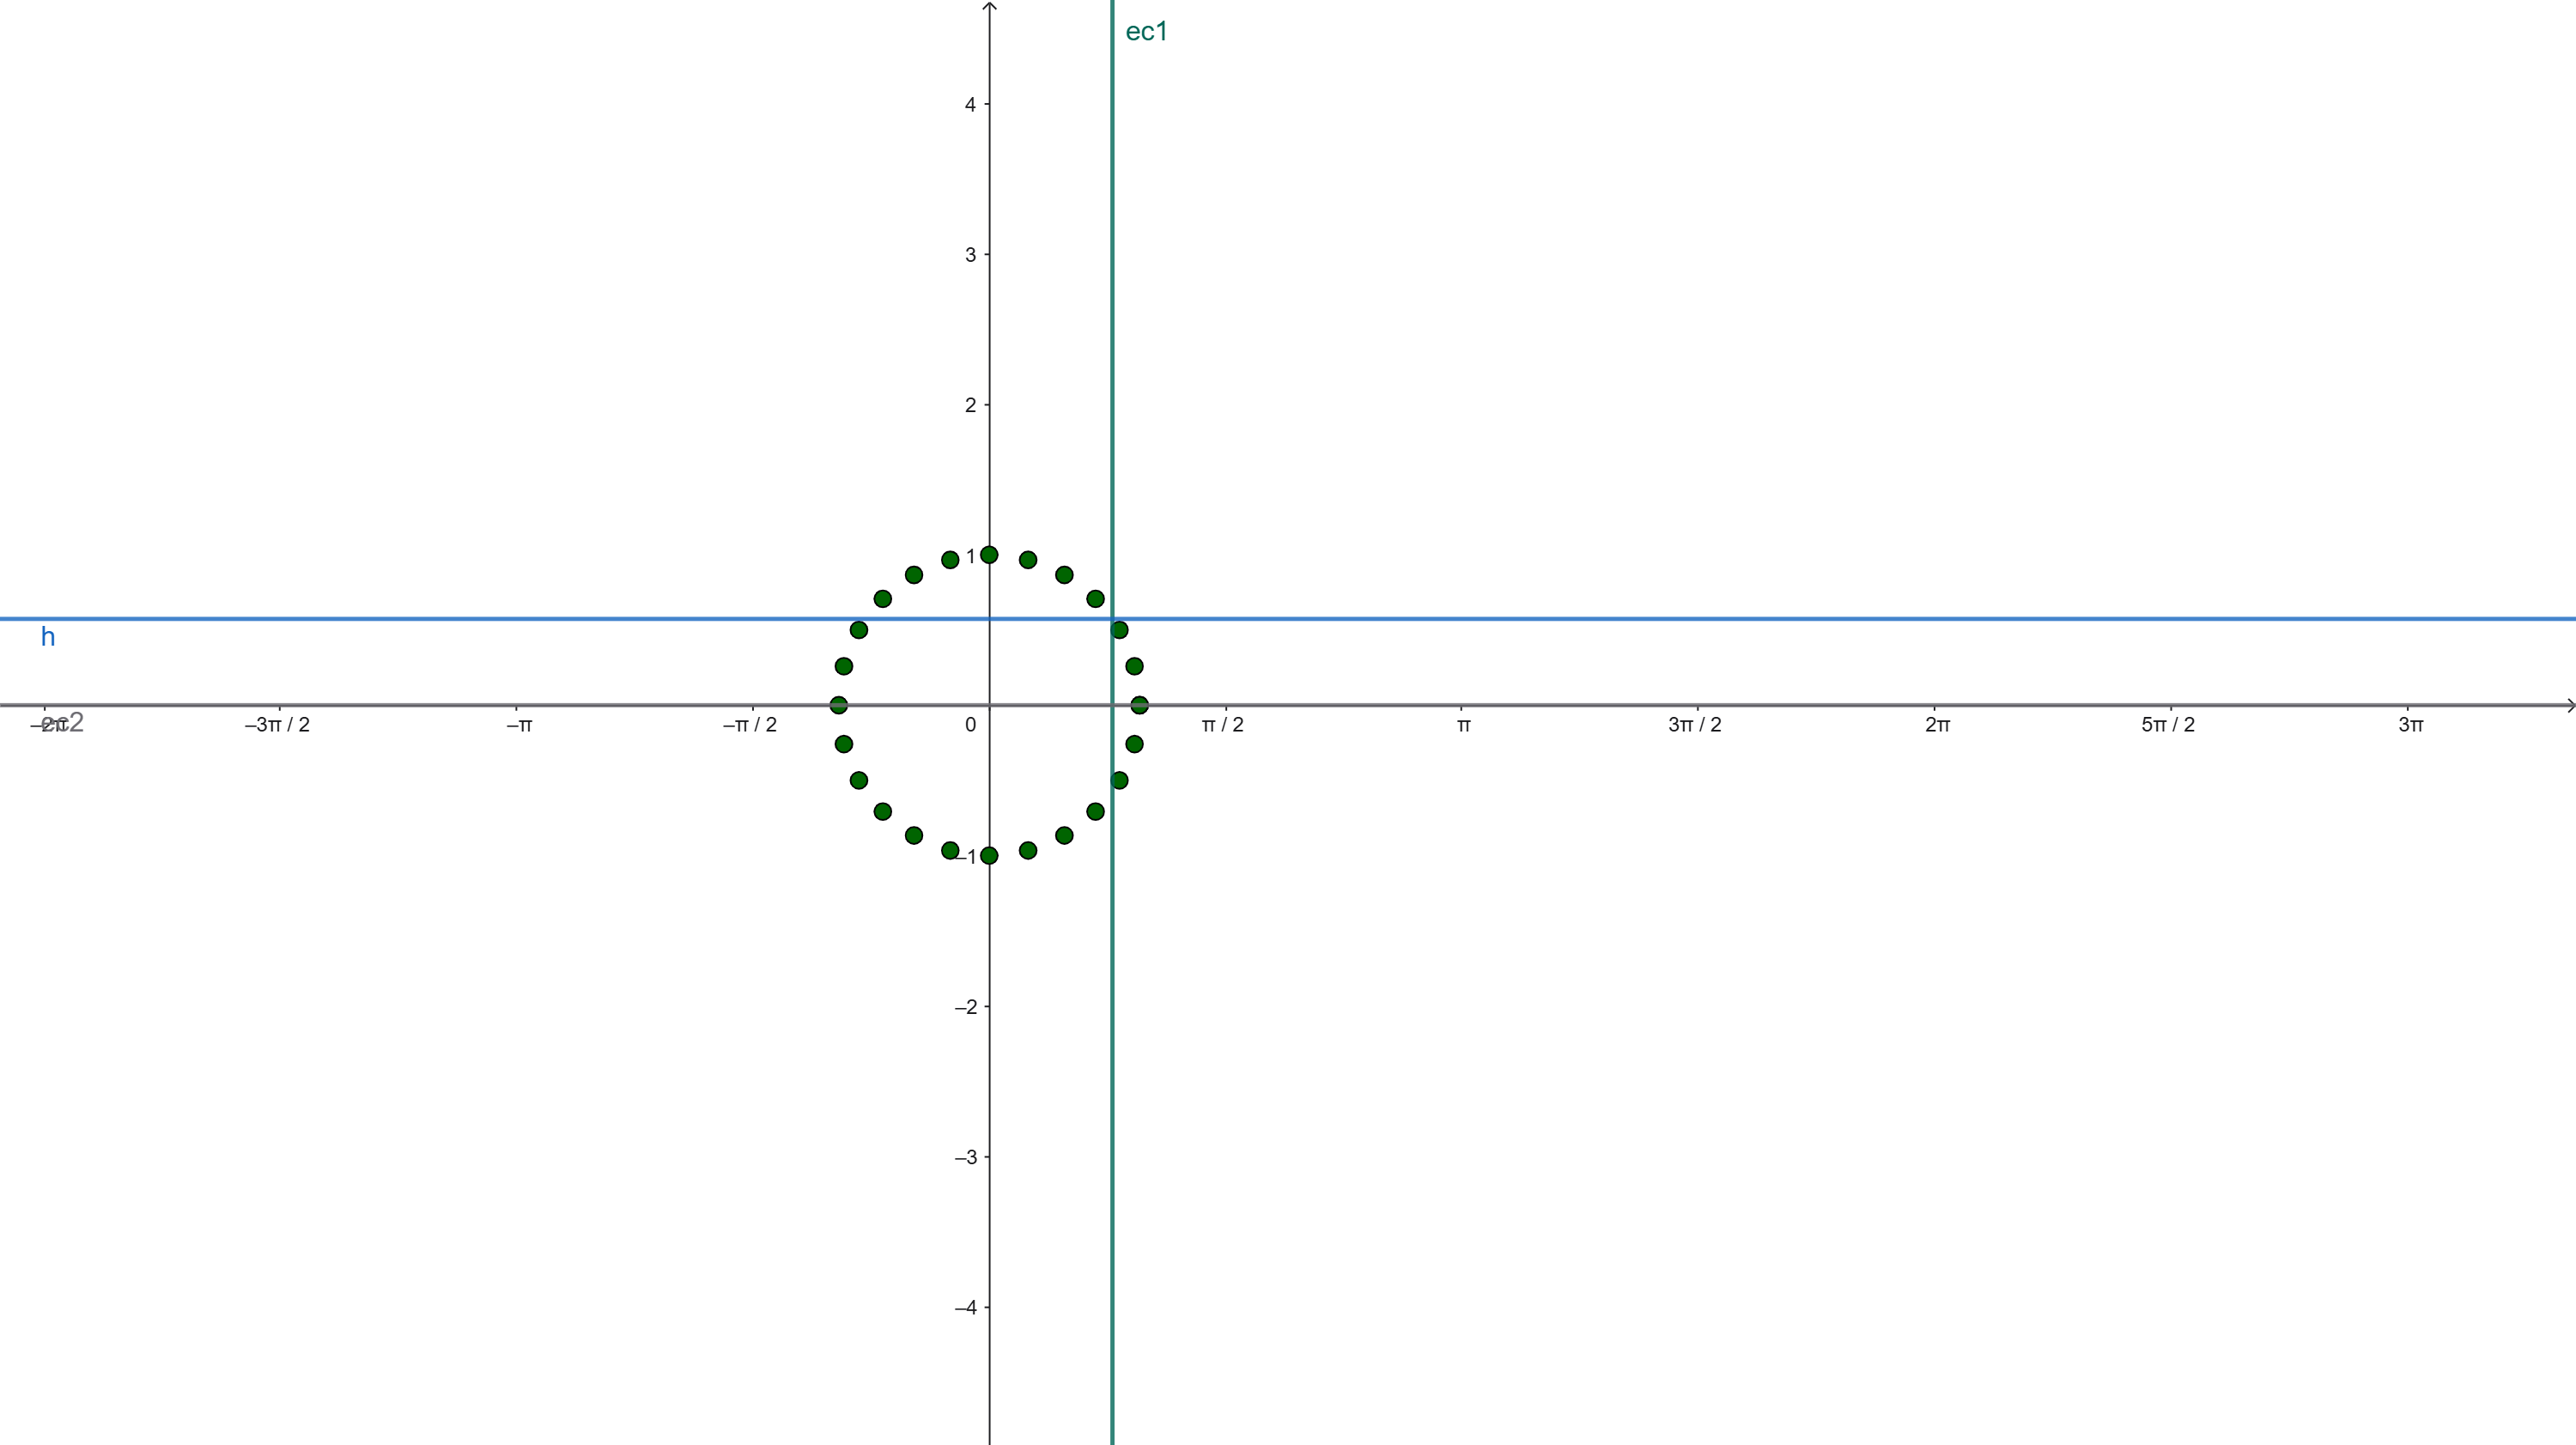
\includegraphics[width=0.55\textwidth]{Apendices/rc.png}
  \caption{Visualización discreta del comportamiento cíclico del tiempo} 
  \caption*{GeoGebra: Generación de puntos discretos sobre la circunferencia usando la expresión: \newline
  \texttt{Sequence((cos(2$\pi$ * n / 86400), sin(2$\pi$ * n / 86400)), n, 0, 86400, 3600)}}
  \caption*{La figura incluye dos líneas auxiliares que recorren la circunferencia: una horizontal (coseno) y una vertical (seno), generadas dinámicamente mediante un deslizador \( t \) con paso de 600 segundos. Estas líneas intersectan en el punto \( (x, y) \), representando la posición temporal proyectada en coordenadas trigonométricas.}
  \label{fig:representacion-ciclica-tiempo}
\end{figure}

\begin{figure}[ht!]
  \centering
  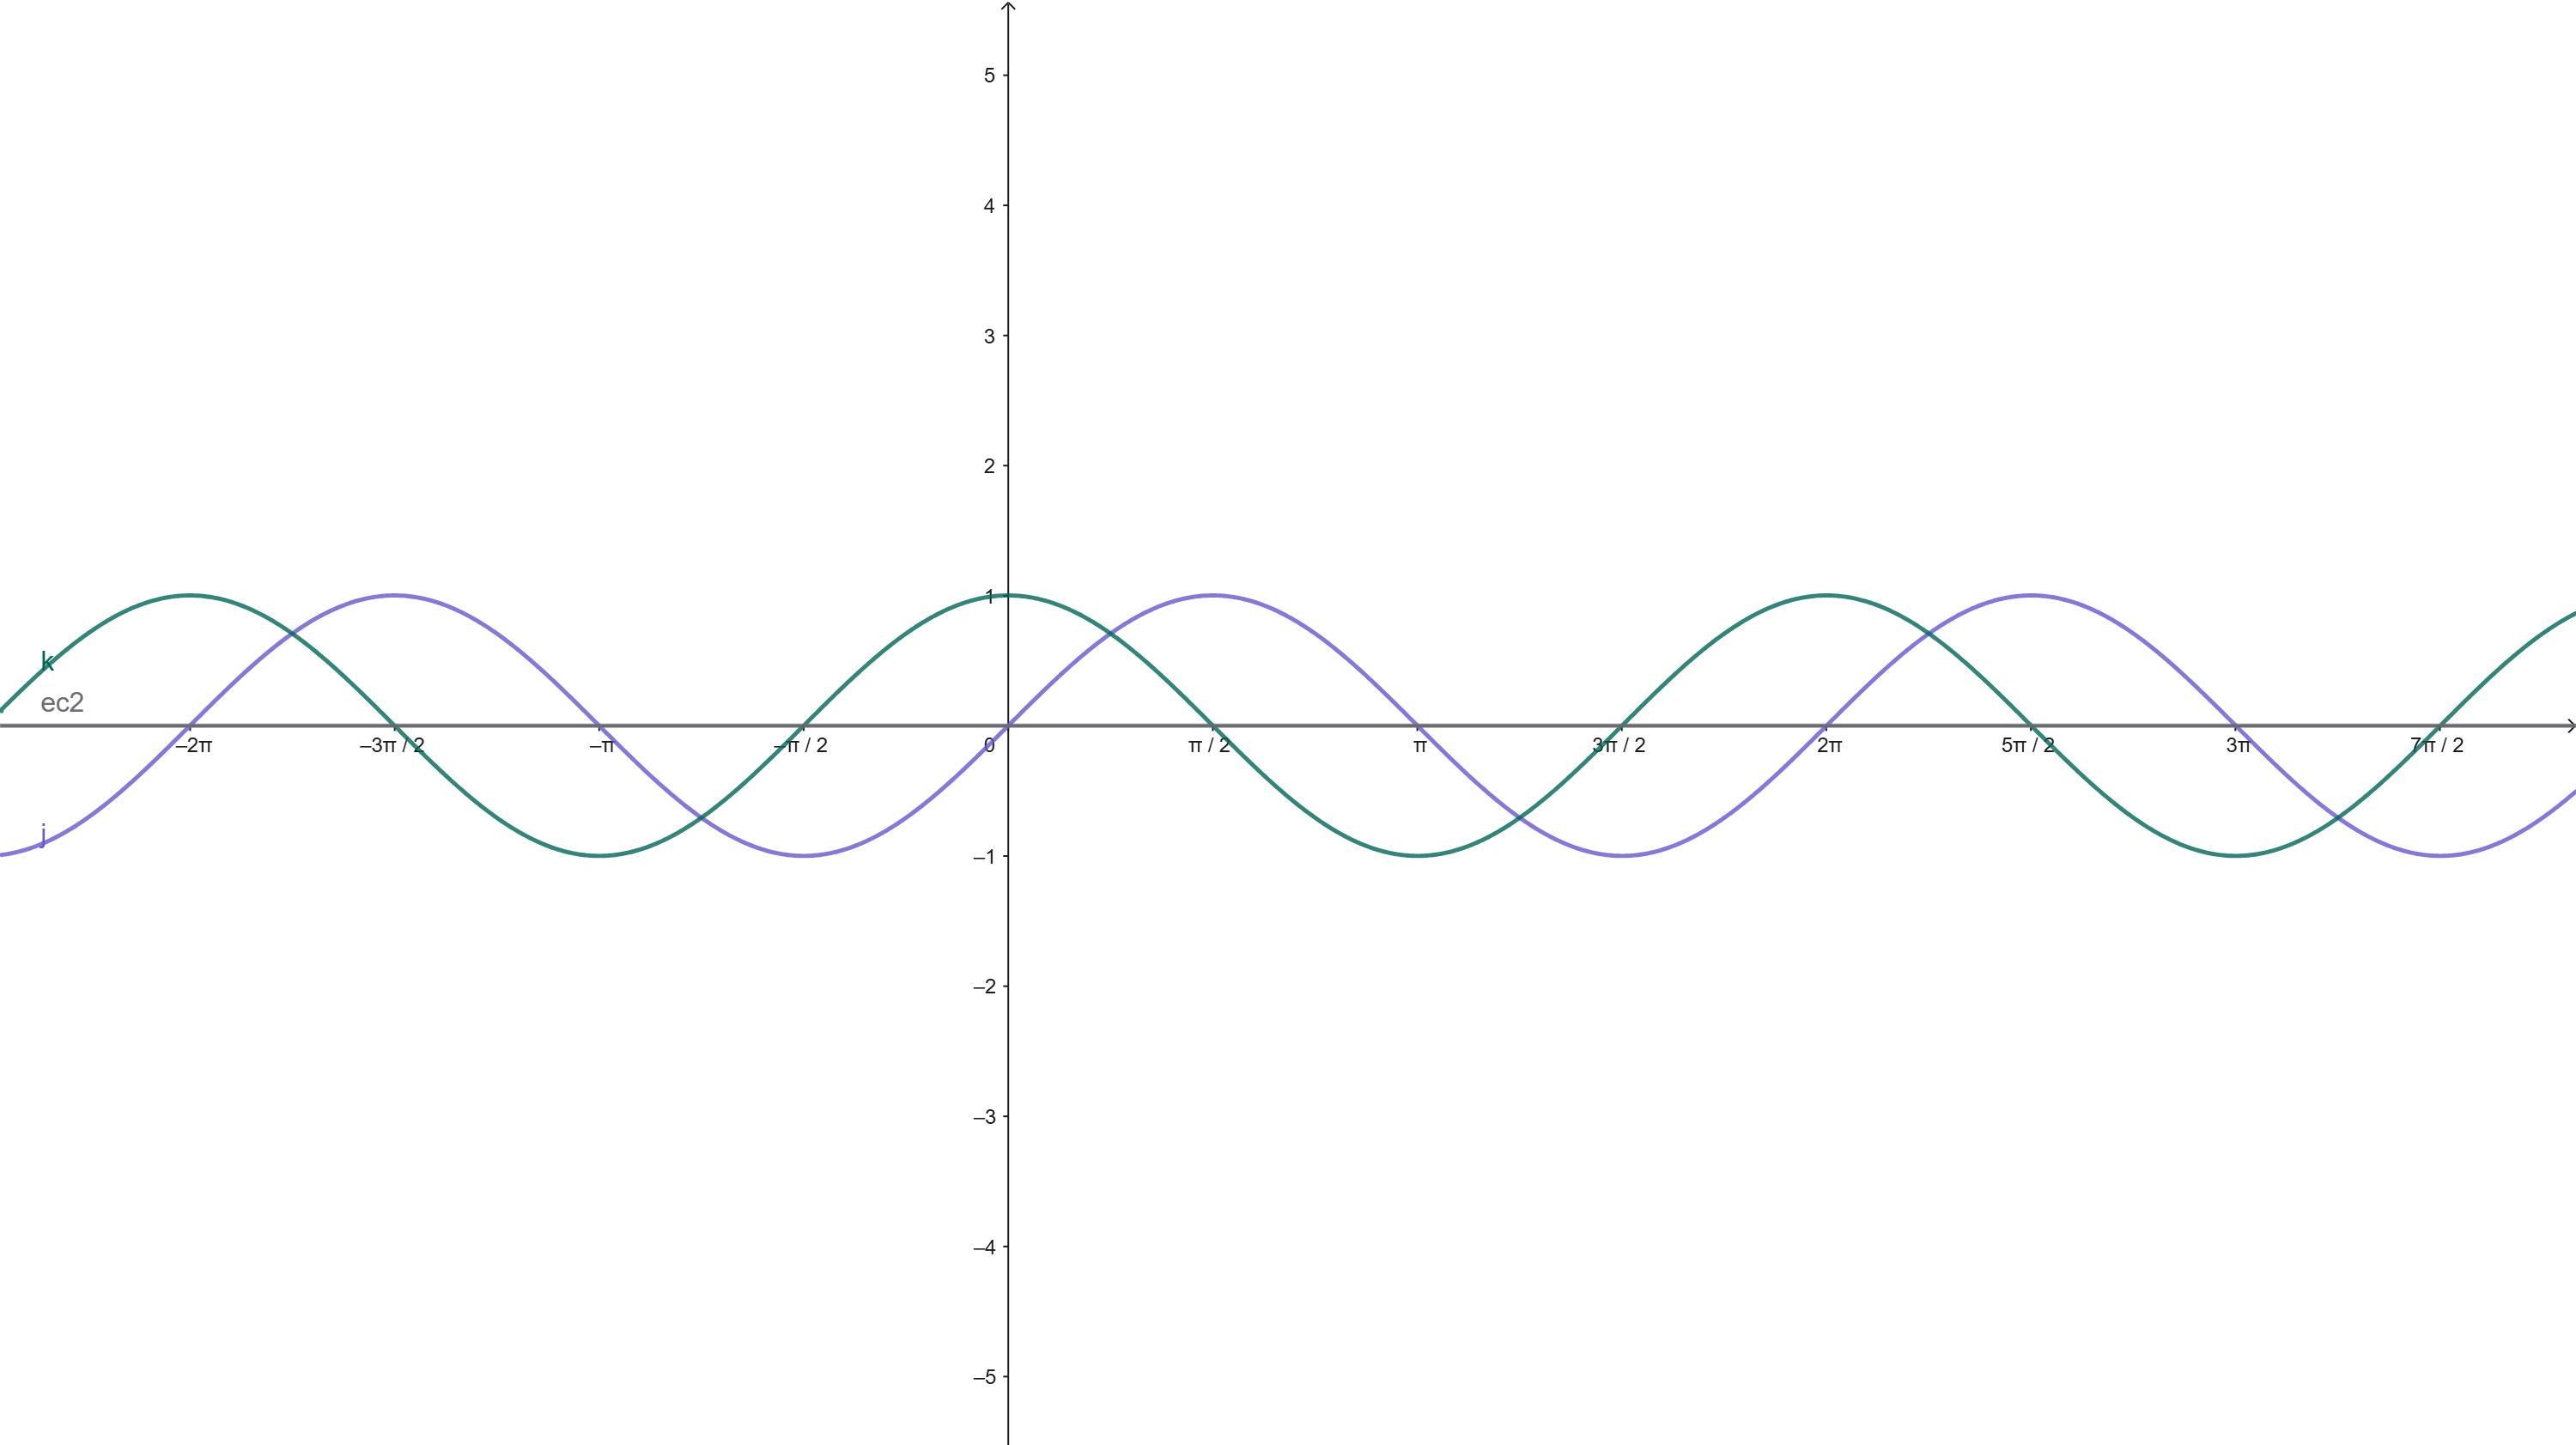
\includegraphics[width=0.55\textwidth]{Apendices/sencos.png}
  \caption{Visualización de las funciones seno y coseno  } 
  \caption*{GeoGebra: Generación de las funciones seno y coseno usando las expresiones: \newline
  \texttt{Sequence((x, sin(x)), x, 0, 2$\pi$, $\pi$/6)} y \newline
  \texttt{Sequence((x, cos(x)), x, 0, 2$\pi$, $\pi$/6)}}
  \label{fig: seno-coseno}
\end{figure}

\begin{figure}[ht!]
  \centering
  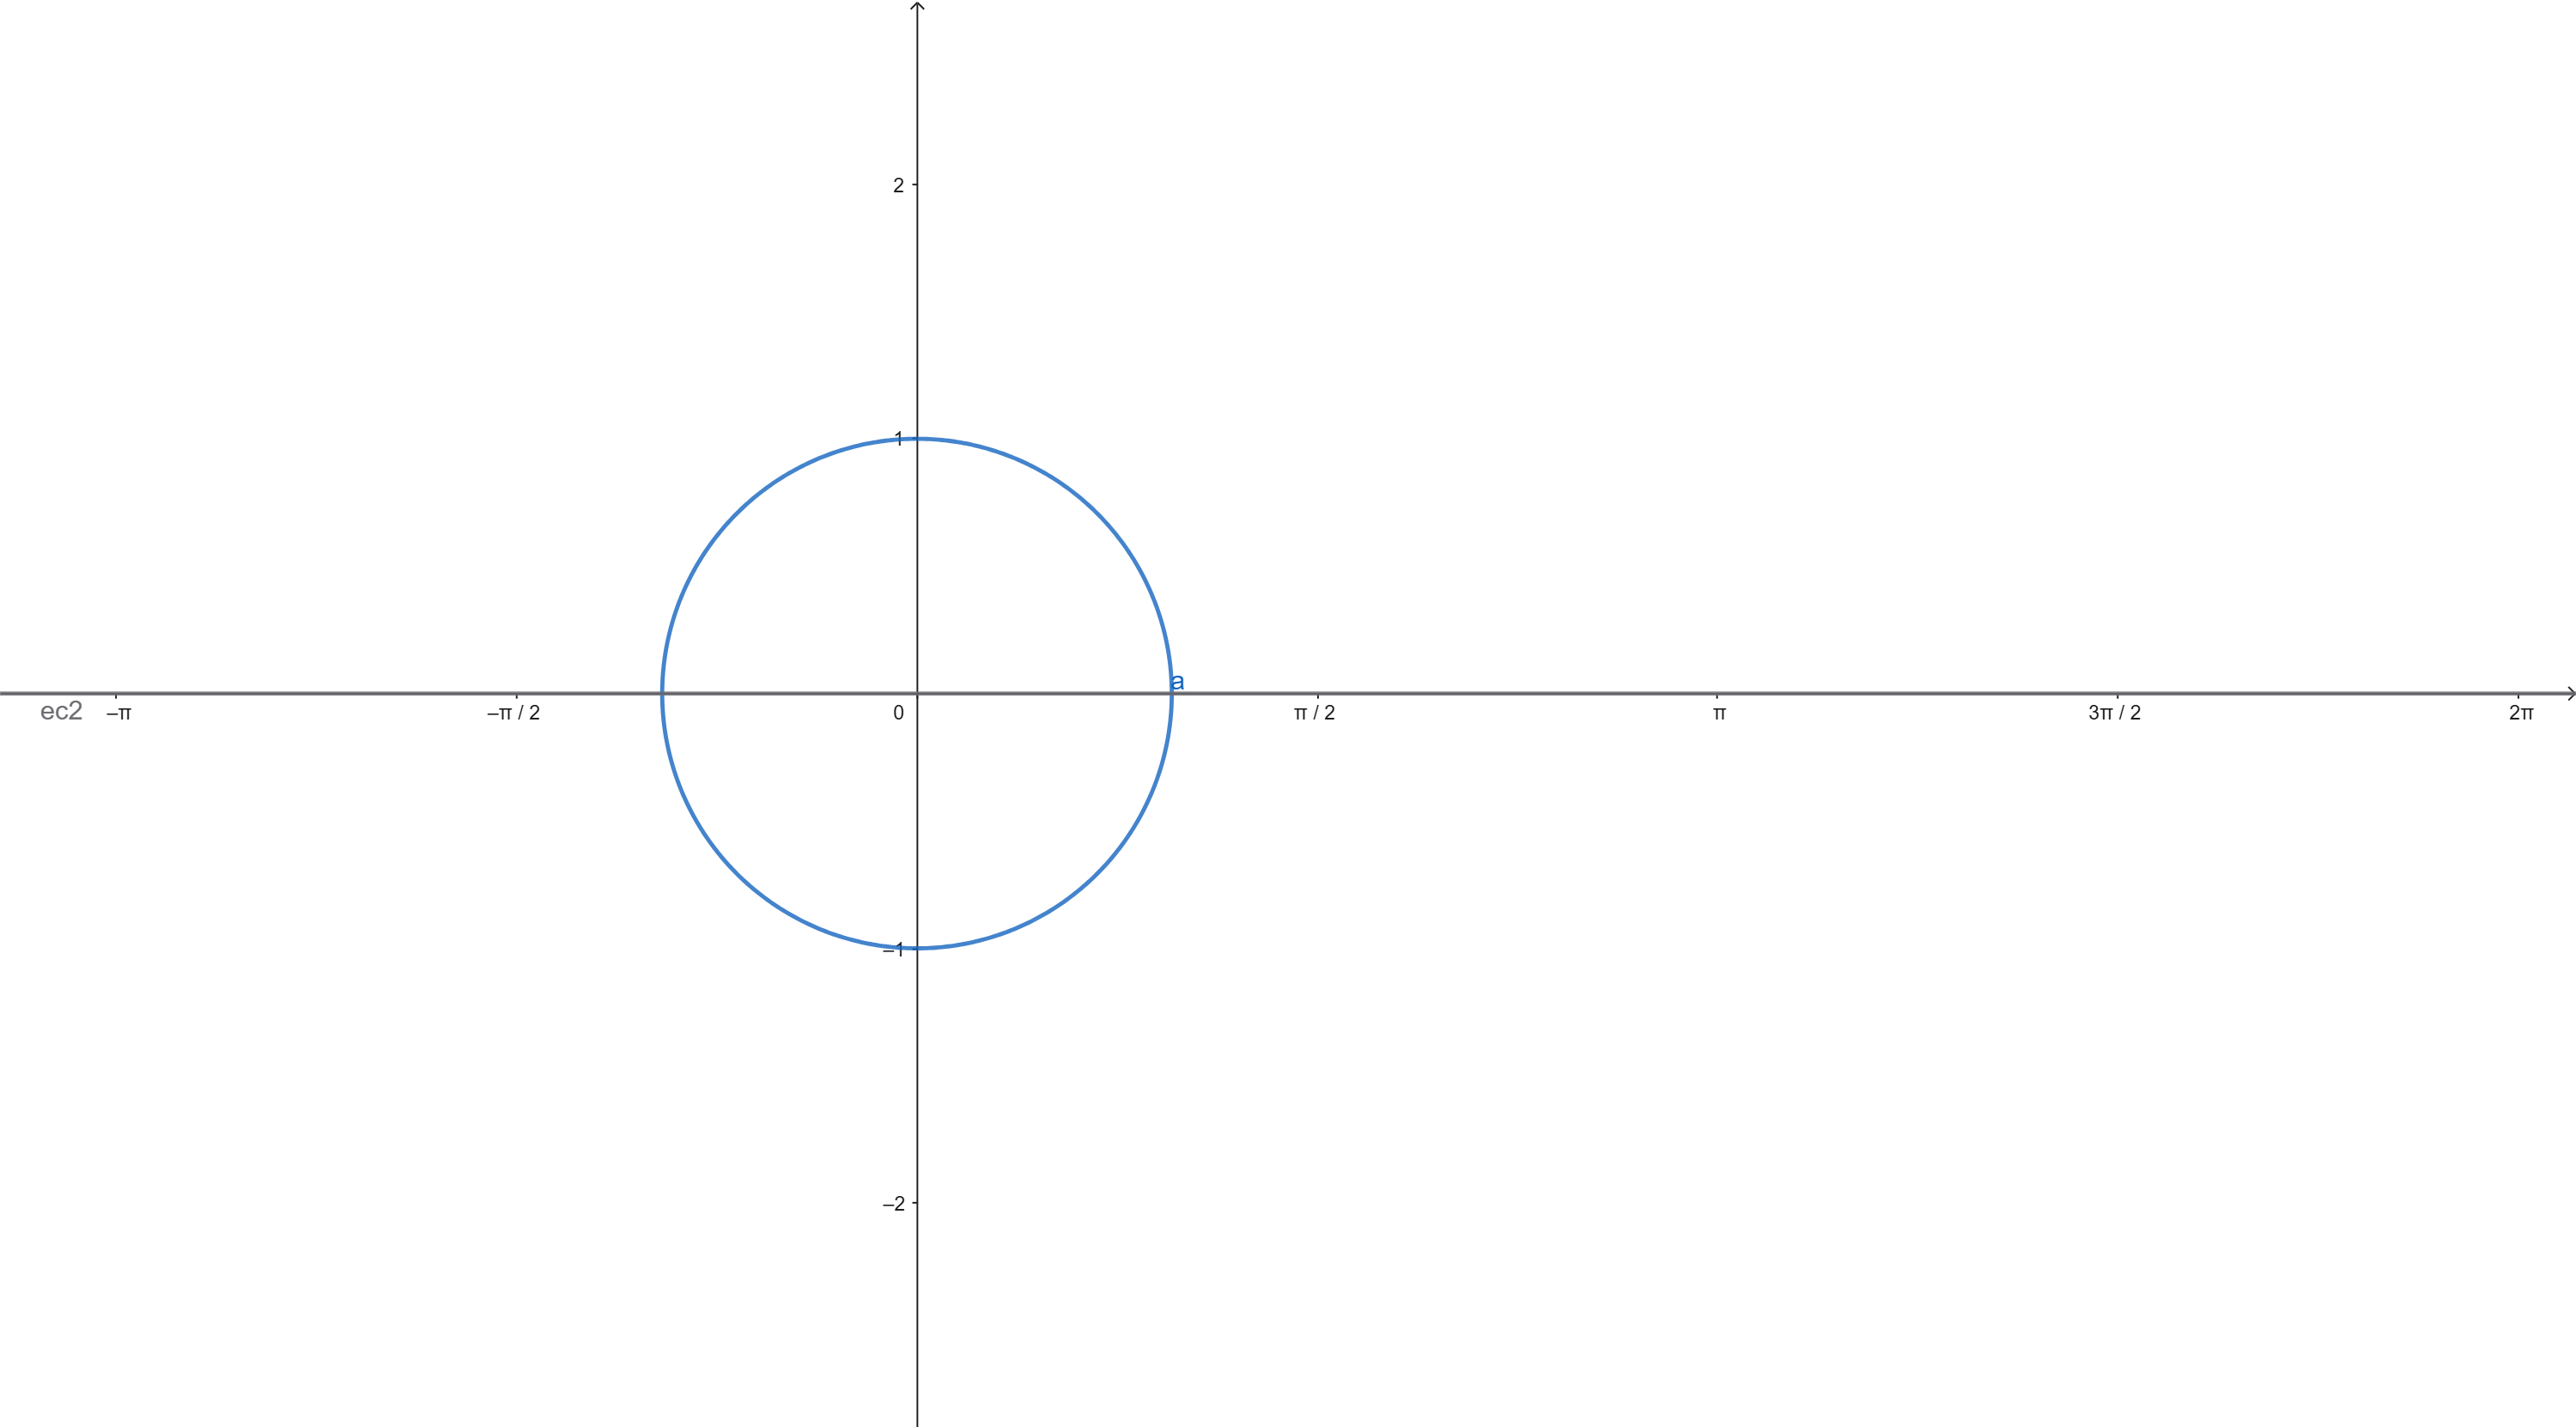
\includegraphics[width=0.55\textwidth]{Apendices/curve.png}
  \caption{Curva paramétrica continua del tiempo sobre el círculo unitario}
  \caption*{GeoGebra: Generación de la curva mediante las expresiones: \newline
  \texttt{x(t) = cos(2$\pi$ * t / 86400)}, \quad
  \texttt{y(t) = sin(2$\pi$ * t / 86400)}, \quad
  \texttt{Curve(x(t), y(t), t, 0, 86400)}}
  \caption*{La figura muestra una curva paramétrica continua que representa el tiempo sobre el círculo unitario mediante funciones trigonométricas. Cada instante se proyecta como un punto único definido por \( x(t) = \cos\left(\frac{2\pi t}{86400}\right) \) y \( y(t) = \sin\left(\frac{2\pi t}{86400}\right) \), donde \( t \) es el número de segundos desde las 00:00. Esta codificación garantiza continuidad angular, permitiendo que modelos de simulación o aprendizaje automático interpreten correctamente la naturaleza cíclica del tiempo sin ambigüedades en los extremos del día.}
  \label{fig:curva-tiempo-circular}
\end{figure}
\uextra{Apendice}{Verificación del sistema de monitoreo acústico}

{\small
  \begin{longtable}[c]{c p{3.5cm} p{2.2cm} p{2.2cm} p{3.5cm}}
    \hline
    \textbf{Requerimiento} & \textbf{Descripción}                                                                                    & \textbf{Entrada}                                                  & \textbf{Salida}                                                       & \textbf{Criterio de Aceptación}                                                       \\
    \hline
    \endfirsthead

    \hline
    \textbf{Requerimiento} & \textbf{Descripción}                                                                                    & \textbf{Entrada}                                                  & \textbf{Salida}                                                       & \textbf{Criterio de Aceptación}                                                       \\
    \hline
    \endhead
    \endfoot
    \endlastfoot

    R1                     & Captura continua del audio ambiental a través de micrófonos.                                            & Señales de audio del entorno a través del hardware del micrófono. & Eventos discretos etiquedados del audio.                              & El sistema debe estar activo y registrando datos en todo momento.                     \\
    \addlinespace
    R2                     & Procesamiento del audio para clasificarlo en eventos sonoros predefinidos.                              & Flujo de datos de audio.                                          & Clasificación del sonido (ej. voz, silencio, golpe).                  & El sistema debe etiquetar correctamente la señal de audio que recibe en todo momento. \\
    \addlinespace
    R3                     & El sistema debe conocer en todo momento el estado de actividad del entorno.                             & Señal de audio.                                                   & Hay ruido o silencio.                                                 & El sistema reconoce cuando hay ruido o silencio.                                      \\
    \addlinespace
    R4                     & Comparación de la actividad en tiempo real con el perfil de normalidad para detectar patrones anómalos. & Secuencia de eventos en tiempo real                               & Identificación de una anomalía o evento atípico.                      & Detectar si una secuencia de eventos es normal o anómala.                             \\
    \addlinespace
    R5                     & El sistema realiza una consulta verbal al usuario al detectar una anomalía.                             & Señal de audio.                                                   & Emisión de una pregunta de voz pregrabada (ej. ``¿Está todo bien?''). & El sistema consulta el estado del usuario antes de enviar una alerta.                 \\
    \addlinespace
    R6                     & Permitir cancelar una alerta de emergencia por comando de voz.                                          & Respuesta de voz del usuario (ej. ``Estoy bien'').                & No se envía alerta.                                                   & El sistema cancela la alerta.                                                         \\
    \addlinespace
    R7                     & El sistema envía notificaciones de emergencia si la anomalía es crítica o el usuario no responde.       & Falta de respuesta del usuario o gravedad de la anomalía          & Envío de notificaciones.                                              & El sistema es capaz de enviar una alerta sin la intervención del usuario.             \\
    \bottomrule
    \addlinespace

    \caption{Requerimientos del sistema acústico}
    \label{tab:requerimientos_sistema_acustico}
  \end{longtable}
}

\titleformat{\chapter}
{\normalfont\fontsize{12}{15}\centering}{Anexos \thechapter.}{0.3em}{}[]

\clearpage
\thispagestyle{empty}
\begin{center}
  \vspace*{\fill}
  \phantomsection
  Apéndices
  \addcontentsline{toc}{chapter}{Anexos}
  \vspace*{\fill}
\end{center}
\clearpage

\appendix
% \uextra{Apendice}{Dispositivo Raspberry Pi 4 Model B}
% \begin{figure}[ht!]
%   \centering
%   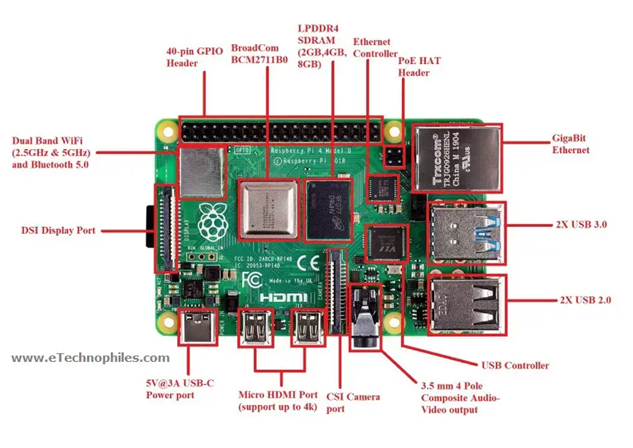
\includegraphics[width=0.95\textwidth]{Anexos/1.arquitectura-raspberry.png}
%   \caption{Arquitectura del Raspberry Pi 4 Model B}
%   \label{fig:raspberry-architecture}
% \end{figure}

\uextra{Apendice}{Representación cíclica del tiempo mediante funciones trigonométricas}
\begin{figure}[ht!]
  \centering
  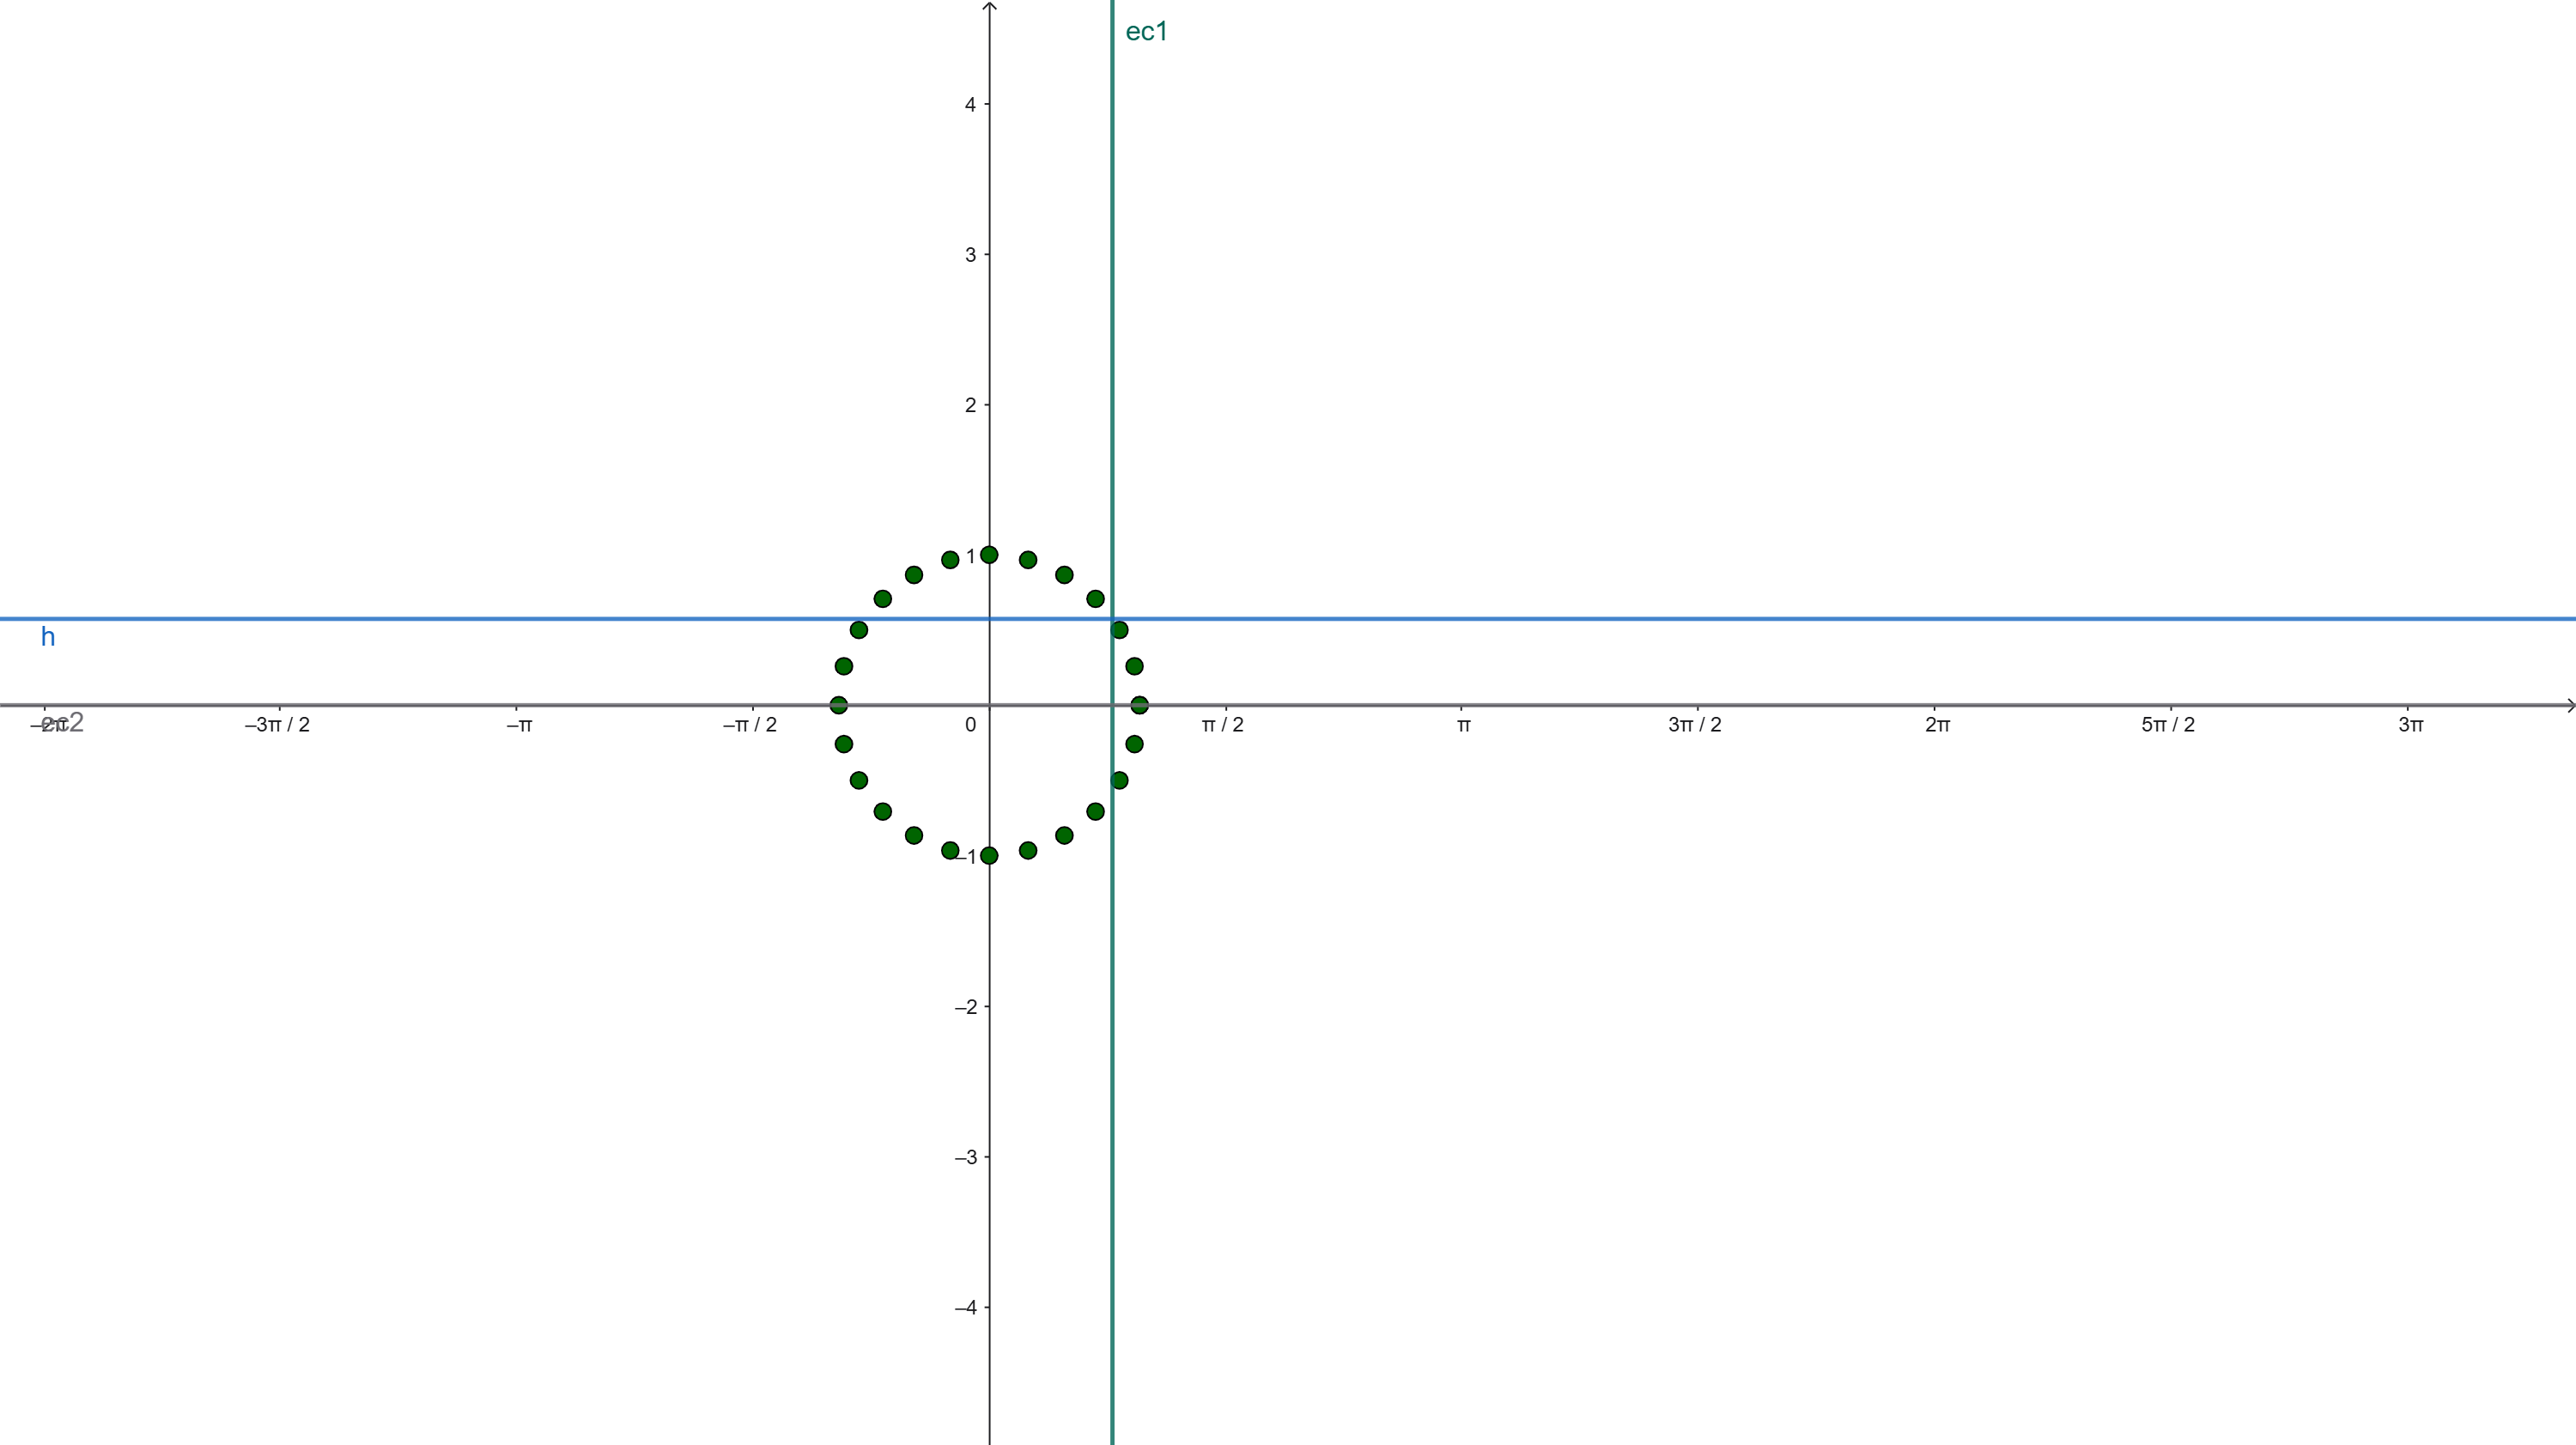
\includegraphics[width=0.55\textwidth]{Apendices/rc.png}
  \caption{Visualización discreta del comportamiento cíclico del tiempo} 
  \caption*{GeoGebra: Generación de puntos discretos sobre la circunferencia usando la expresión: \newline
  \texttt{Sequence((cos(2$\pi$ * n / 86400), sin(2$\pi$ * n / 86400)), n, 0, 86400, 3600)}}
  \caption*{La figura incluye dos líneas auxiliares que recorren la circunferencia: una horizontal (coseno) y una vertical (seno), generadas dinámicamente mediante un deslizador \( t \) con paso de 600 segundos. Estas líneas intersectan en el punto \( (x, y) \), representando la posición temporal proyectada en coordenadas trigonométricas.}
  \label{fig:representacion-ciclica-tiempo}
\end{figure}

\begin{figure}[ht!]
  \centering
  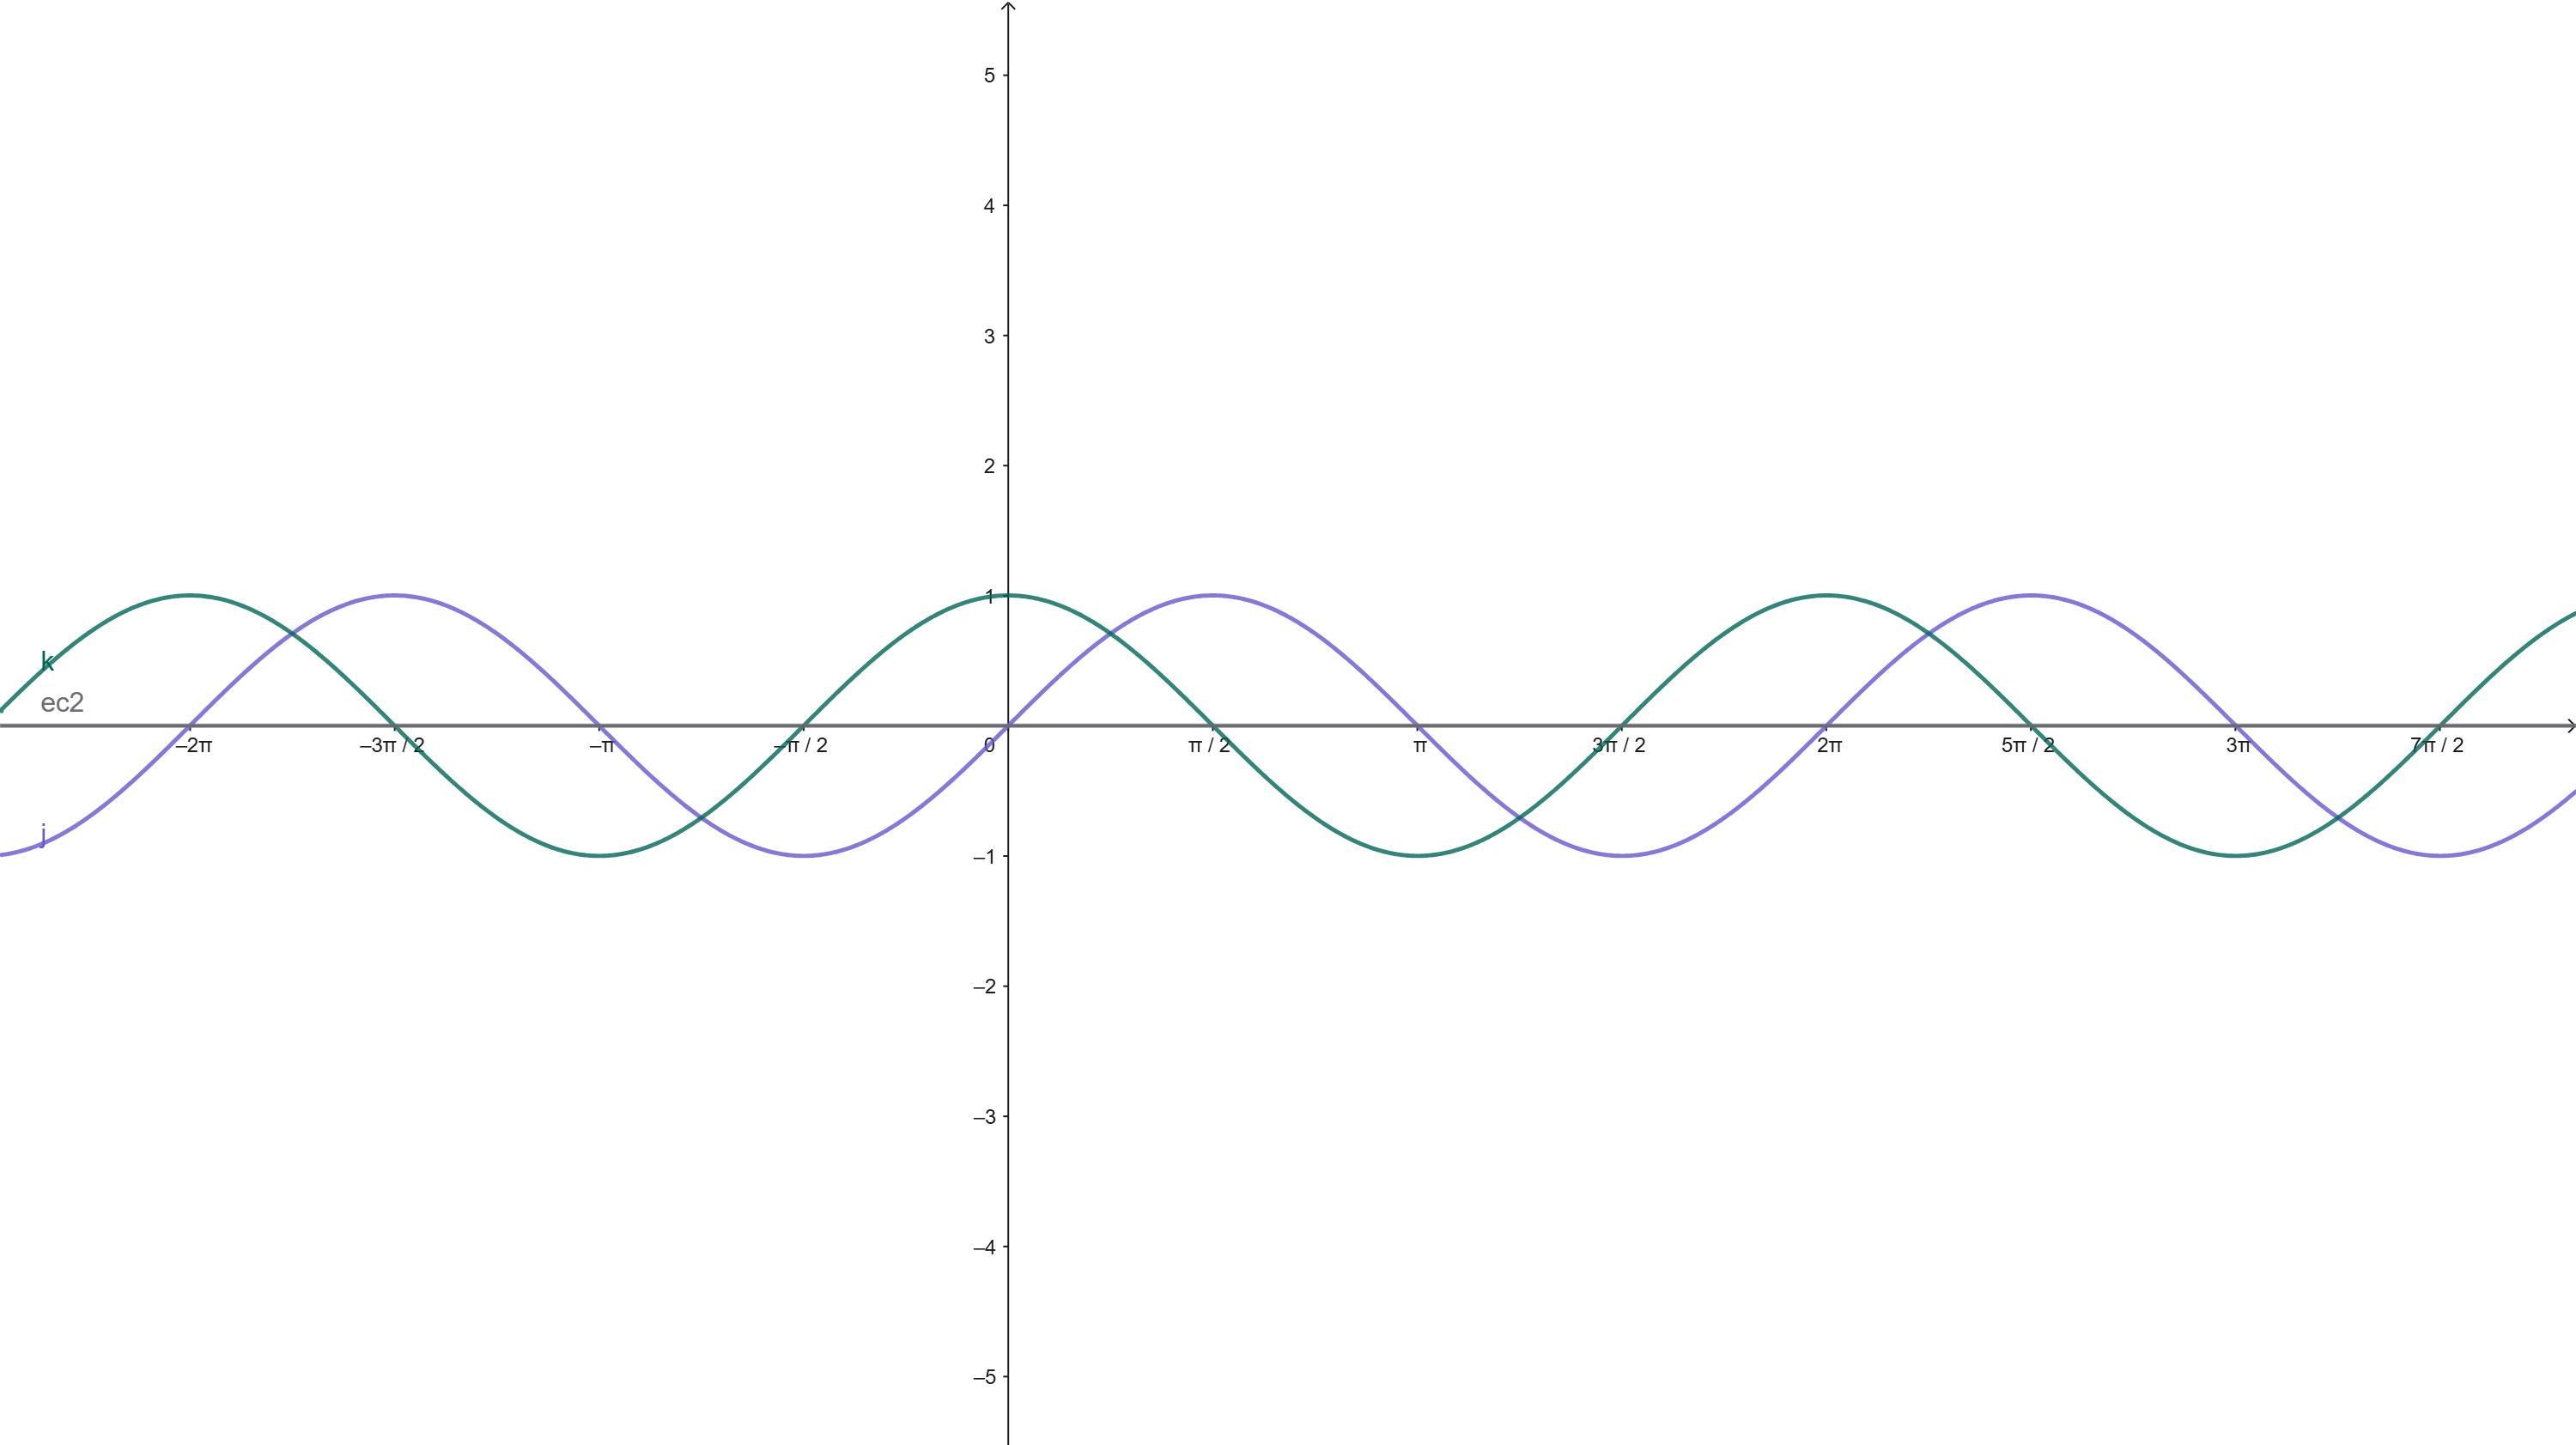
\includegraphics[width=0.55\textwidth]{Apendices/sencos.png}
  \caption{Visualización de las funciones seno y coseno  } 
  \caption*{GeoGebra: Generación de las funciones seno y coseno usando las expresiones: \newline
  \texttt{Sequence((x, sin(x)), x, 0, 2$\pi$, $\pi$/6)} y \newline
  \texttt{Sequence((x, cos(x)), x, 0, 2$\pi$, $\pi$/6)}}
  \label{fig: seno-coseno}
\end{figure}

\begin{figure}[ht!]
  \centering
  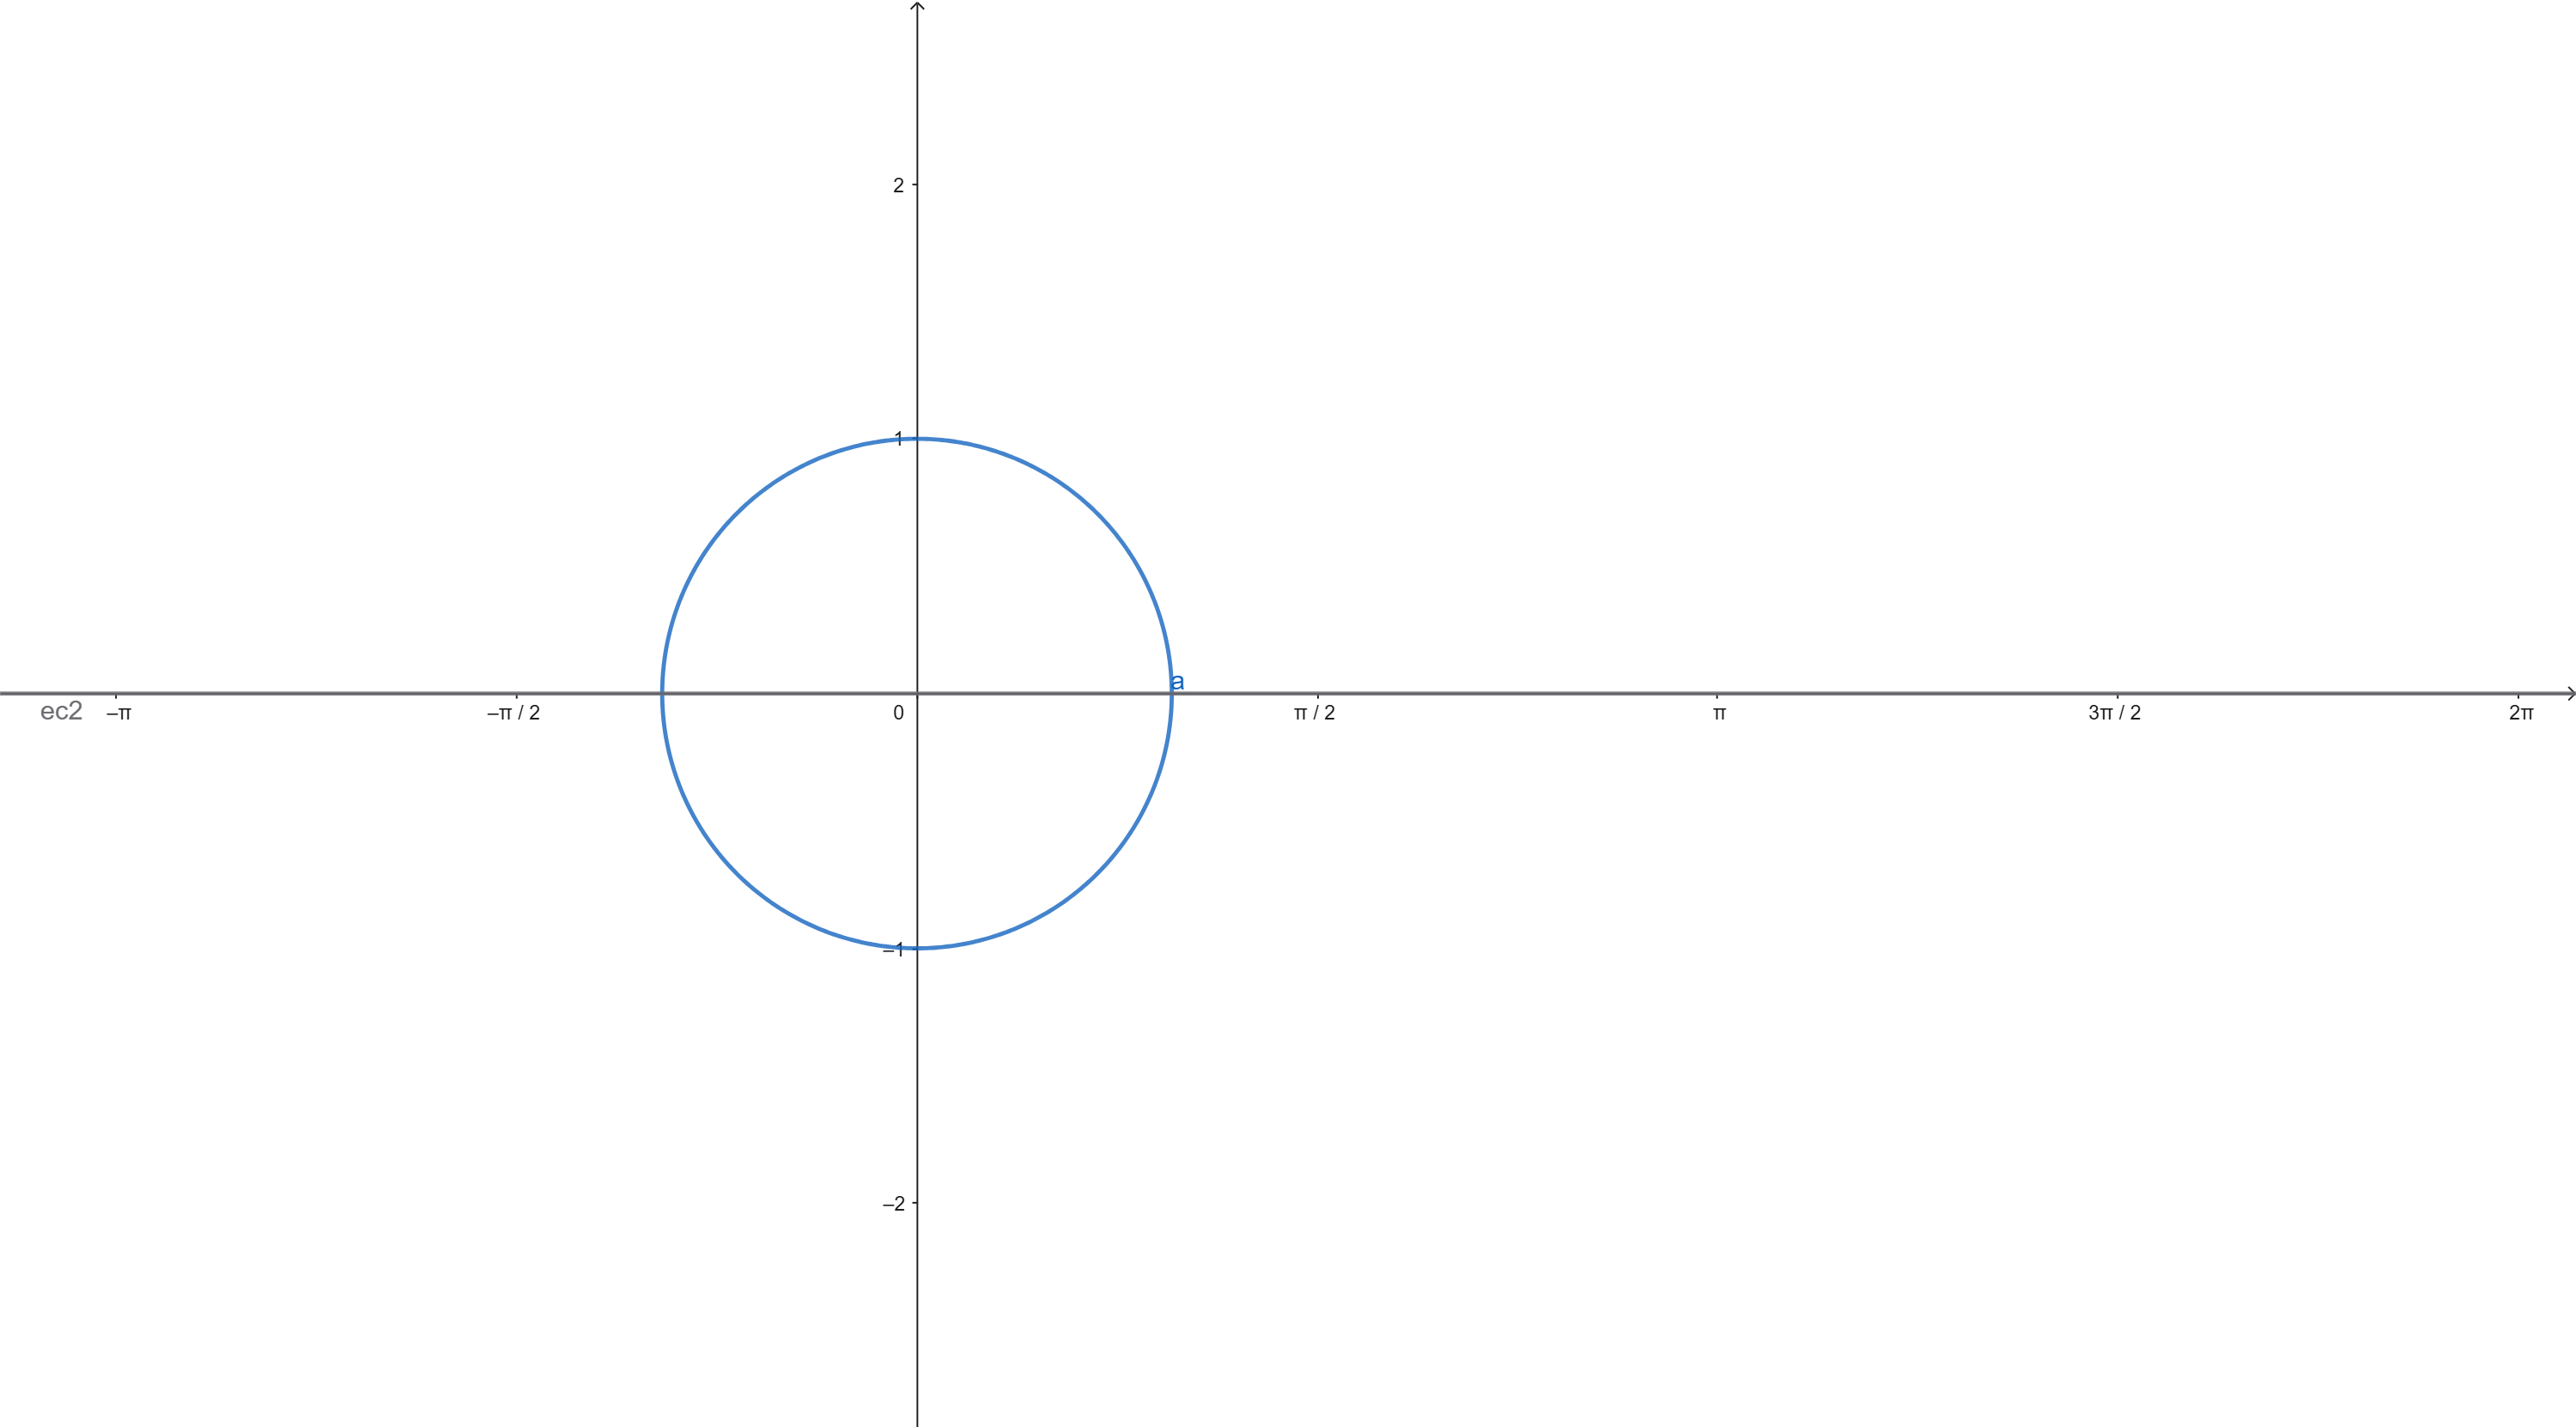
\includegraphics[width=0.55\textwidth]{Apendices/curve.png}
  \caption{Curva paramétrica continua del tiempo sobre el círculo unitario}
  \caption*{GeoGebra: Generación de la curva mediante las expresiones: \newline
  \texttt{x(t) = cos(2$\pi$ * t / 86400)}, \quad
  \texttt{y(t) = sin(2$\pi$ * t / 86400)}, \quad
  \texttt{Curve(x(t), y(t), t, 0, 86400)}}
  \caption*{La figura muestra una curva paramétrica continua que representa el tiempo sobre el círculo unitario mediante funciones trigonométricas. Cada instante se proyecta como un punto único definido por \( x(t) = \cos\left(\frac{2\pi t}{86400}\right) \) y \( y(t) = \sin\left(\frac{2\pi t}{86400}\right) \), donde \( t \) es el número de segundos desde las 00:00. Esta codificación garantiza continuidad angular, permitiendo que modelos de simulación o aprendizaje automático interpreten correctamente la naturaleza cíclica del tiempo sin ambigüedades en los extremos del día.}
  \label{fig:curva-tiempo-circular}
\end{figure}
\uextra{Apendice}{Verificación del sistema de monitoreo acústico}

{\small
  \begin{longtable}[c]{c p{3.5cm} p{2.2cm} p{2.2cm} p{3.5cm}}
    \hline
    \textbf{Requerimiento} & \textbf{Descripción}                                                                                    & \textbf{Entrada}                                                  & \textbf{Salida}                                                       & \textbf{Criterio de Aceptación}                                                       \\
    \hline
    \endfirsthead

    \hline
    \textbf{Requerimiento} & \textbf{Descripción}                                                                                    & \textbf{Entrada}                                                  & \textbf{Salida}                                                       & \textbf{Criterio de Aceptación}                                                       \\
    \hline
    \endhead
    \endfoot
    \endlastfoot

    R1                     & Captura continua del audio ambiental a través de micrófonos.                                            & Señales de audio del entorno a través del hardware del micrófono. & Eventos discretos etiquedados del audio.                              & El sistema debe estar activo y registrando datos en todo momento.                     \\
    \addlinespace
    R2                     & Procesamiento del audio para clasificarlo en eventos sonoros predefinidos.                              & Flujo de datos de audio.                                          & Clasificación del sonido (ej. voz, silencio, golpe).                  & El sistema debe etiquetar correctamente la señal de audio que recibe en todo momento. \\
    \addlinespace
    R3                     & El sistema debe conocer en todo momento el estado de actividad del entorno.                             & Señal de audio.                                                   & Hay ruido o silencio.                                                 & El sistema reconoce cuando hay ruido o silencio.                                      \\
    \addlinespace
    R4                     & Comparación de la actividad en tiempo real con el perfil de normalidad para detectar patrones anómalos. & Secuencia de eventos en tiempo real                               & Identificación de una anomalía o evento atípico.                      & Detectar si una secuencia de eventos es normal o anómala.                             \\
    \addlinespace
    R5                     & El sistema realiza una consulta verbal al usuario al detectar una anomalía.                             & Señal de audio.                                                   & Emisión de una pregunta de voz pregrabada (ej. ``¿Está todo bien?''). & El sistema consulta el estado del usuario antes de enviar una alerta.                 \\
    \addlinespace
    R6                     & Permitir cancelar una alerta de emergencia por comando de voz.                                          & Respuesta de voz del usuario (ej. ``Estoy bien'').                & No se envía alerta.                                                   & El sistema cancela la alerta.                                                         \\
    \addlinespace
    R7                     & El sistema envía notificaciones de emergencia si la anomalía es crítica o el usuario no responde.       & Falta de respuesta del usuario o gravedad de la anomalía          & Envío de notificaciones.                                              & El sistema es capaz de enviar una alerta sin la intervención del usuario.             \\
    \bottomrule
    \addlinespace

    \caption{Requerimientos del sistema acústico}
    \label{tab:requerimientos_sistema_acustico}
  \end{longtable}
}


\phantomsection
\bibliography{references}

\titleformat{\chapter}
{\normalfont\fontsize{12}{15}\centering}{Anexos \thechapter.}{0.3em}{}[]

\clearpage
\thispagestyle{empty}
\begin{center}
  \vspace*{\fill}
  \phantomsection
  Apéndices
  \addcontentsline{toc}{chapter}{Anexos}
  \vspace*{\fill}
\end{center}
\clearpage

\appendix
% \uextra{Apendice}{Dispositivo Raspberry Pi 4 Model B}
% \begin{figure}[ht!]
%   \centering
%   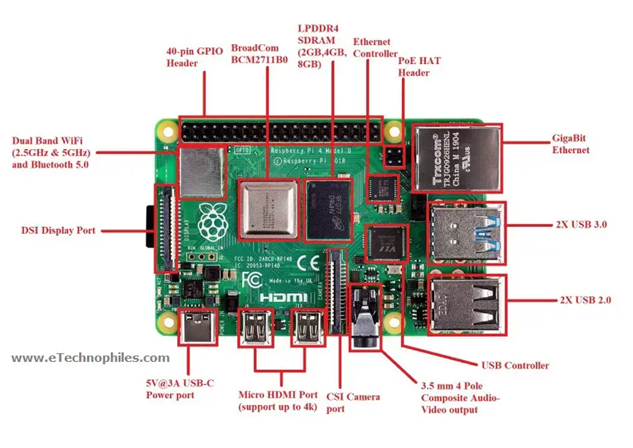
\includegraphics[width=0.95\textwidth]{Anexos/1.arquitectura-raspberry.png}
%   \caption{Arquitectura del Raspberry Pi 4 Model B}
%   \label{fig:raspberry-architecture}
% \end{figure}

\uextra{Apendice}{Representación cíclica del tiempo mediante funciones trigonométricas}
\begin{figure}[ht!]
  \centering
  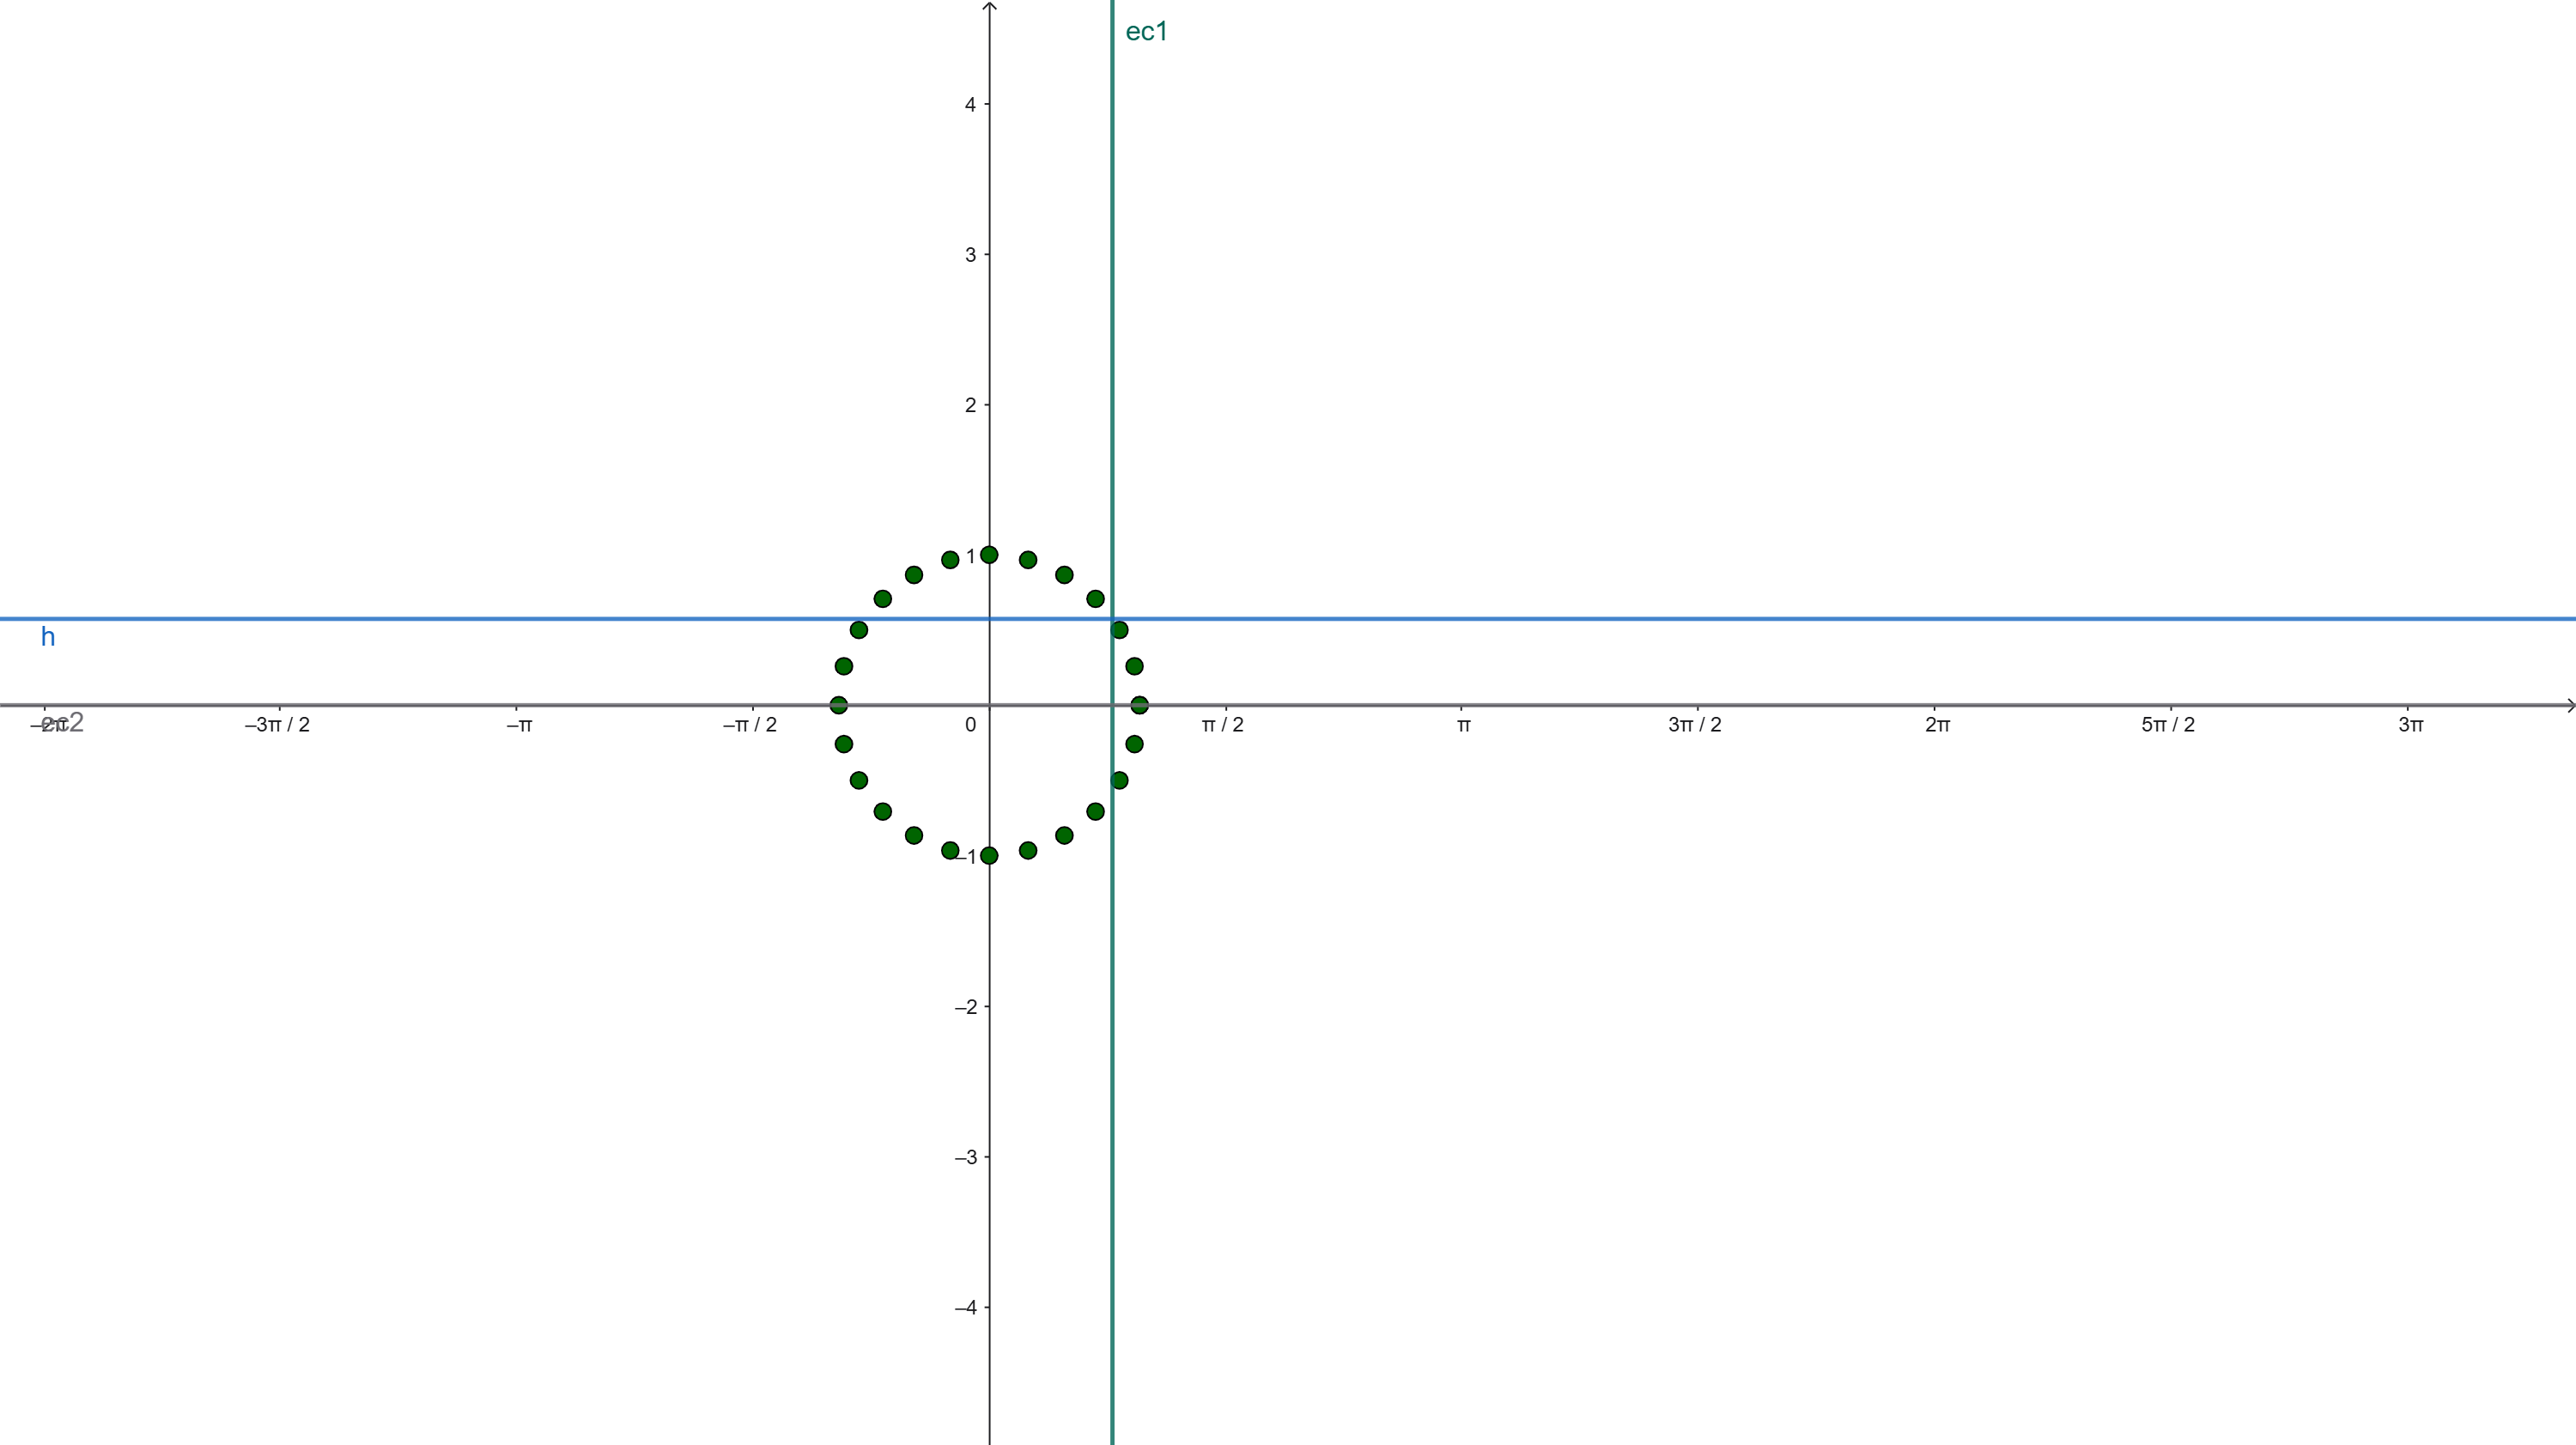
\includegraphics[width=0.55\textwidth]{Apendices/rc.png}
  \caption{Visualización discreta del comportamiento cíclico del tiempo} 
  \caption*{GeoGebra: Generación de puntos discretos sobre la circunferencia usando la expresión: \newline
  \texttt{Sequence((cos(2$\pi$ * n / 86400), sin(2$\pi$ * n / 86400)), n, 0, 86400, 3600)}}
  \caption*{La figura incluye dos líneas auxiliares que recorren la circunferencia: una horizontal (coseno) y una vertical (seno), generadas dinámicamente mediante un deslizador \( t \) con paso de 600 segundos. Estas líneas intersectan en el punto \( (x, y) \), representando la posición temporal proyectada en coordenadas trigonométricas.}
  \label{fig:representacion-ciclica-tiempo}
\end{figure}

\begin{figure}[ht!]
  \centering
  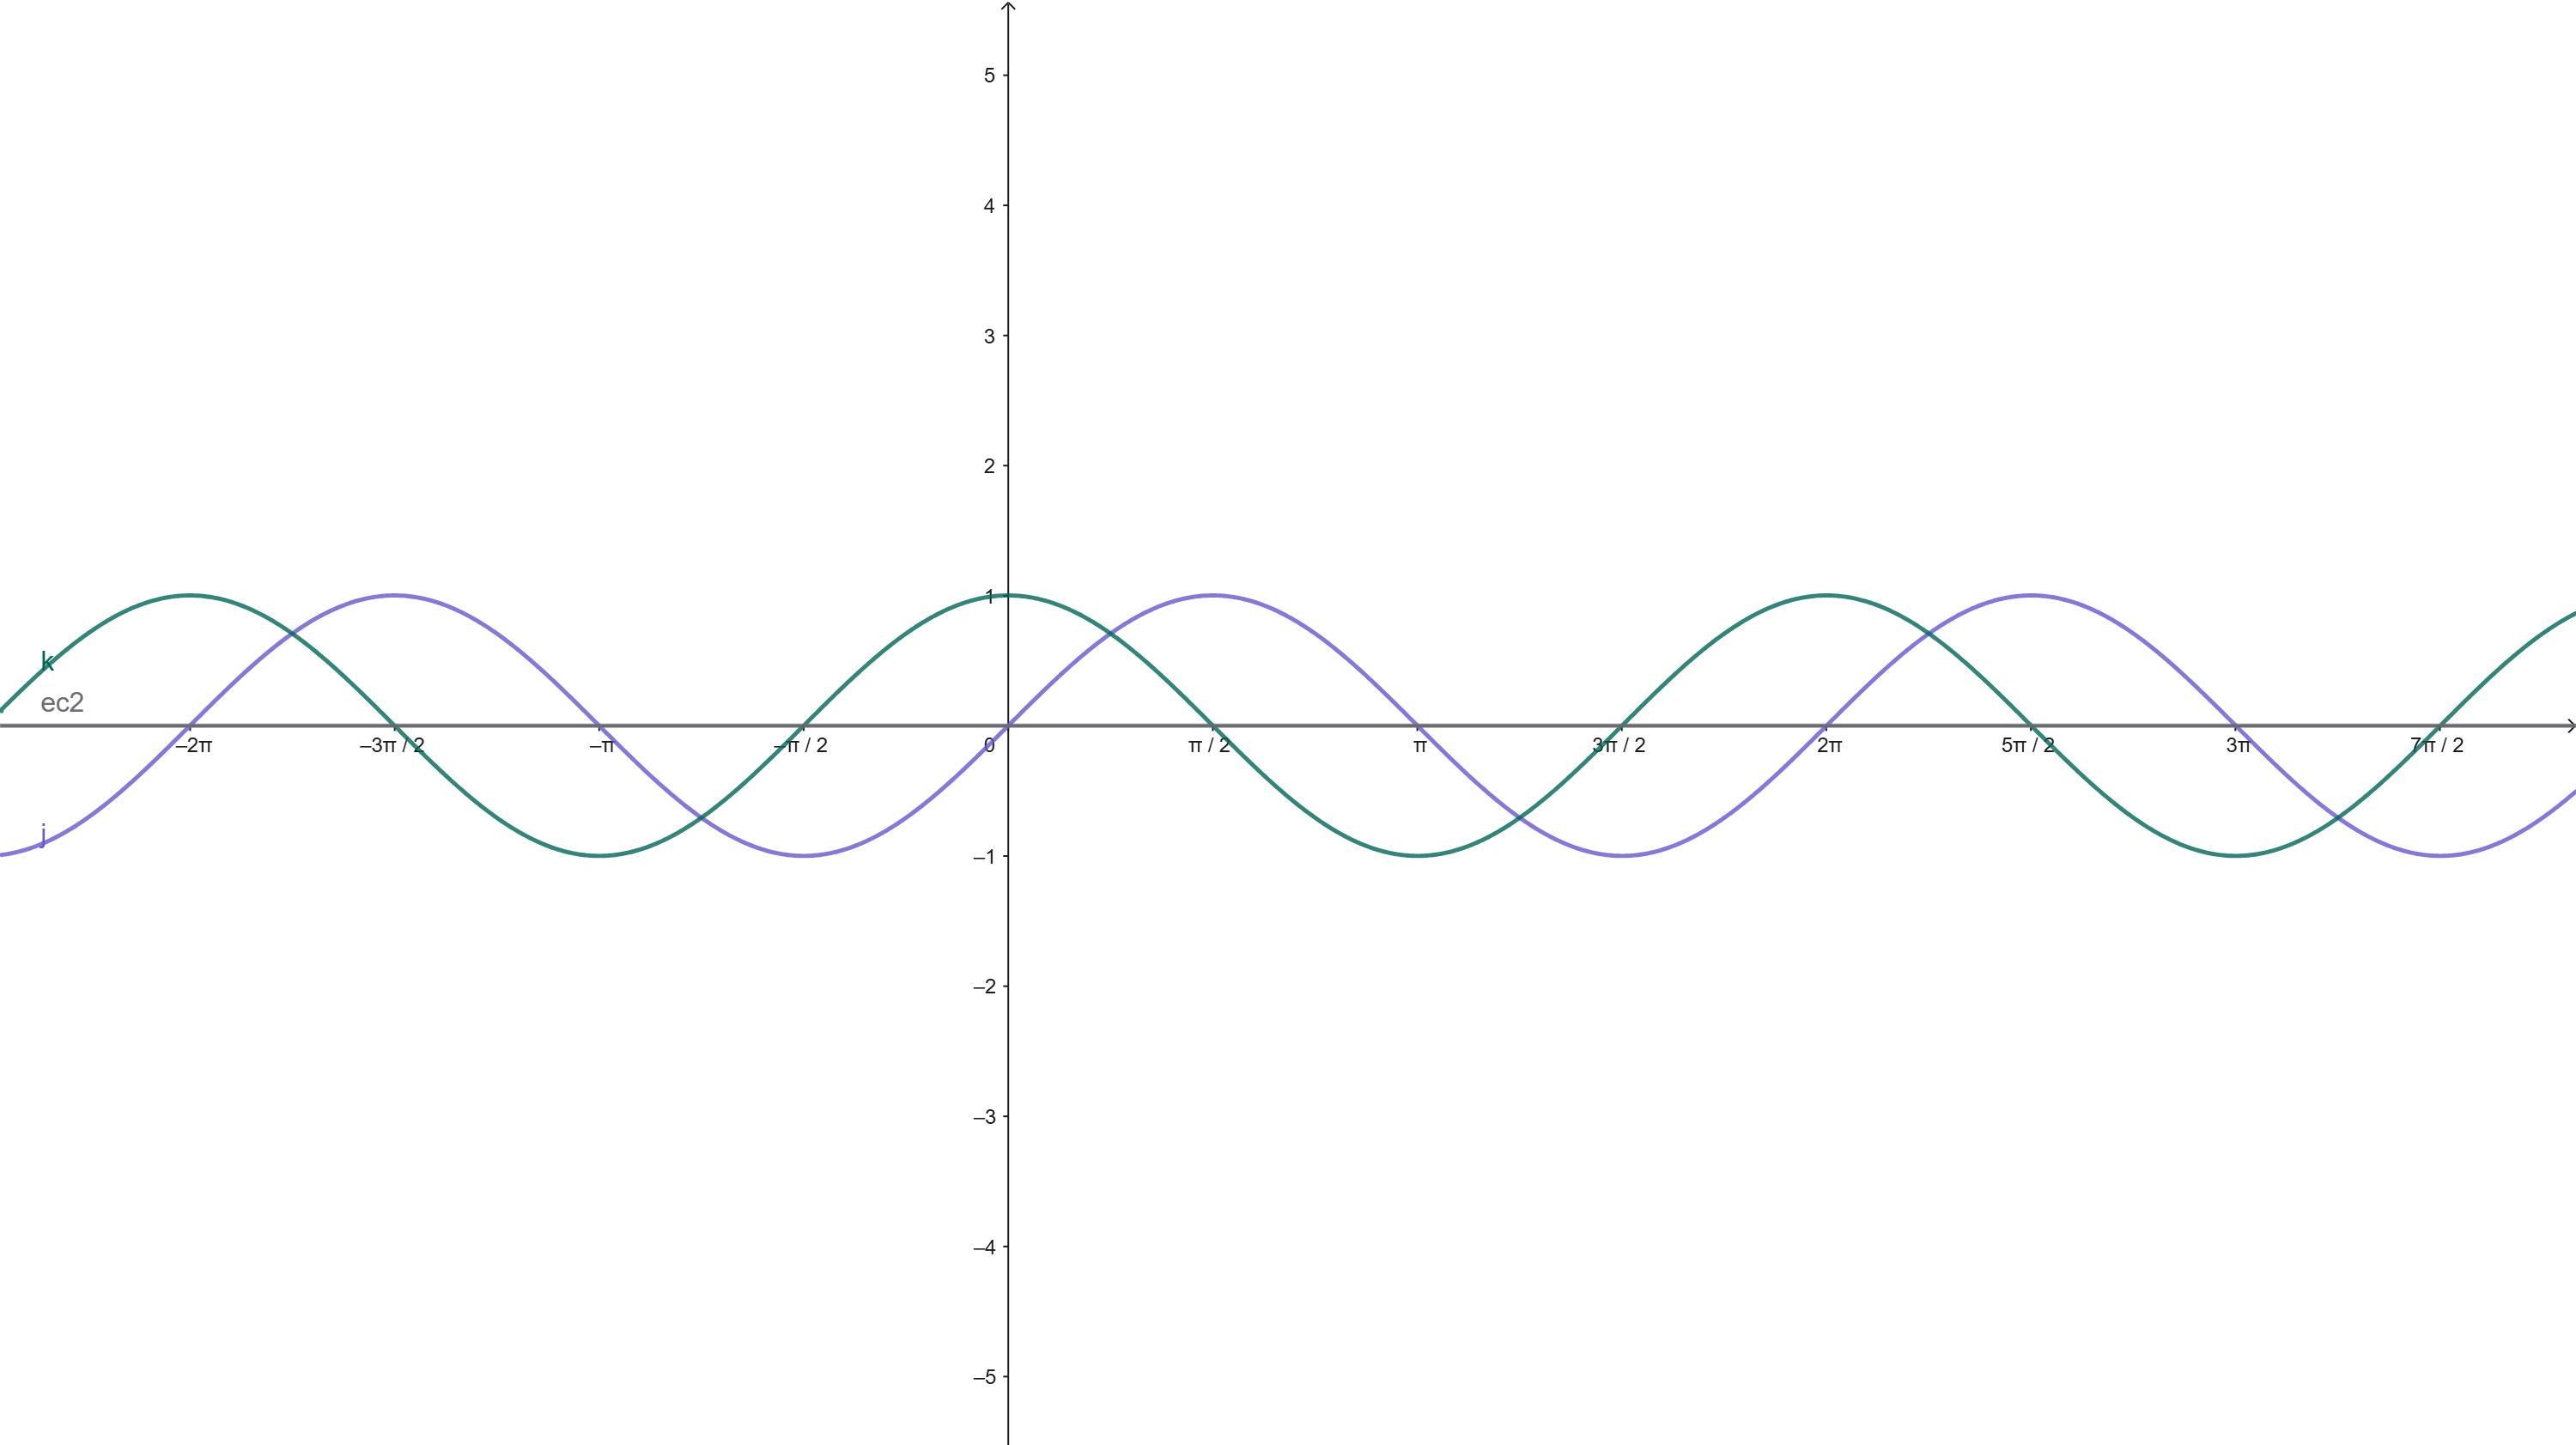
\includegraphics[width=0.55\textwidth]{Apendices/sencos.png}
  \caption{Visualización de las funciones seno y coseno  } 
  \caption*{GeoGebra: Generación de las funciones seno y coseno usando las expresiones: \newline
  \texttt{Sequence((x, sin(x)), x, 0, 2$\pi$, $\pi$/6)} y \newline
  \texttt{Sequence((x, cos(x)), x, 0, 2$\pi$, $\pi$/6)}}
  \label{fig: seno-coseno}
\end{figure}

\begin{figure}[ht!]
  \centering
  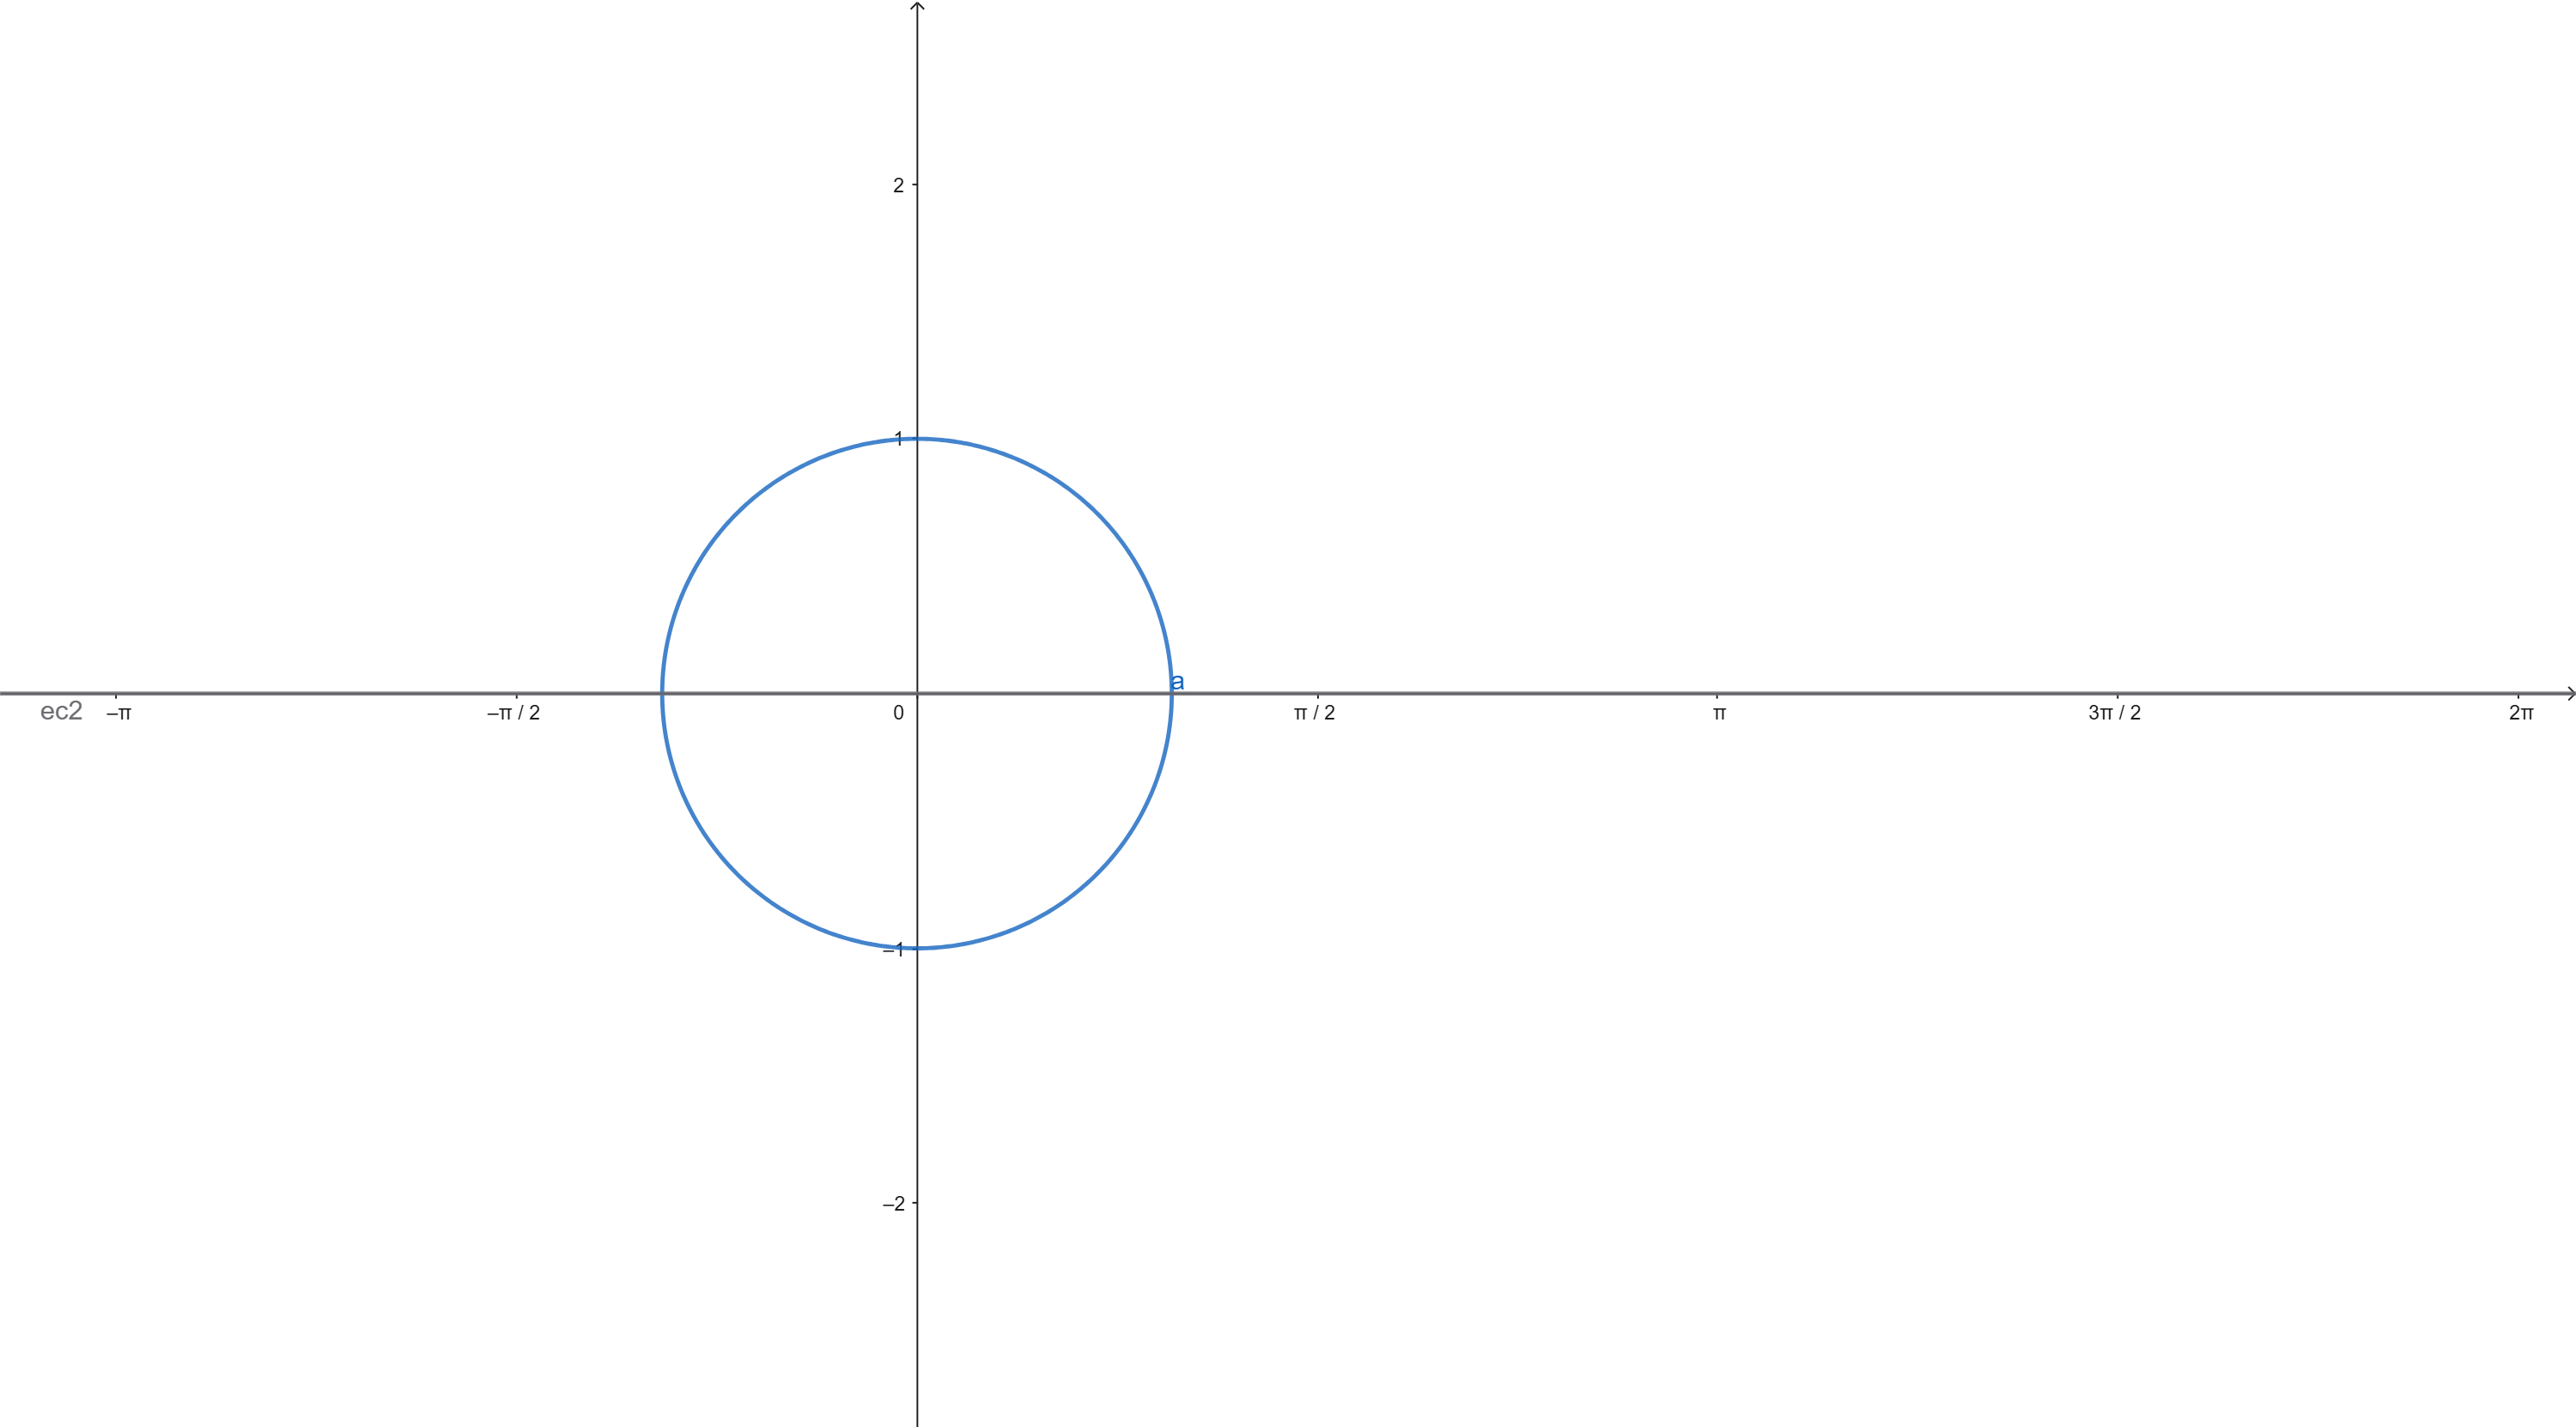
\includegraphics[width=0.55\textwidth]{Apendices/curve.png}
  \caption{Curva paramétrica continua del tiempo sobre el círculo unitario}
  \caption*{GeoGebra: Generación de la curva mediante las expresiones: \newline
  \texttt{x(t) = cos(2$\pi$ * t / 86400)}, \quad
  \texttt{y(t) = sin(2$\pi$ * t / 86400)}, \quad
  \texttt{Curve(x(t), y(t), t, 0, 86400)}}
  \caption*{La figura muestra una curva paramétrica continua que representa el tiempo sobre el círculo unitario mediante funciones trigonométricas. Cada instante se proyecta como un punto único definido por \( x(t) = \cos\left(\frac{2\pi t}{86400}\right) \) y \( y(t) = \sin\left(\frac{2\pi t}{86400}\right) \), donde \( t \) es el número de segundos desde las 00:00. Esta codificación garantiza continuidad angular, permitiendo que modelos de simulación o aprendizaje automático interpreten correctamente la naturaleza cíclica del tiempo sin ambigüedades en los extremos del día.}
  \label{fig:curva-tiempo-circular}
\end{figure}
\uextra{Apendice}{Verificación del sistema de monitoreo acústico}

{\small
  \begin{longtable}[c]{c p{3.5cm} p{2.2cm} p{2.2cm} p{3.5cm}}
    \hline
    \textbf{Requerimiento} & \textbf{Descripción}                                                                                    & \textbf{Entrada}                                                  & \textbf{Salida}                                                       & \textbf{Criterio de Aceptación}                                                       \\
    \hline
    \endfirsthead

    \hline
    \textbf{Requerimiento} & \textbf{Descripción}                                                                                    & \textbf{Entrada}                                                  & \textbf{Salida}                                                       & \textbf{Criterio de Aceptación}                                                       \\
    \hline
    \endhead
    \endfoot
    \endlastfoot

    R1                     & Captura continua del audio ambiental a través de micrófonos.                                            & Señales de audio del entorno a través del hardware del micrófono. & Eventos discretos etiquedados del audio.                              & El sistema debe estar activo y registrando datos en todo momento.                     \\
    \addlinespace
    R2                     & Procesamiento del audio para clasificarlo en eventos sonoros predefinidos.                              & Flujo de datos de audio.                                          & Clasificación del sonido (ej. voz, silencio, golpe).                  & El sistema debe etiquetar correctamente la señal de audio que recibe en todo momento. \\
    \addlinespace
    R3                     & El sistema debe conocer en todo momento el estado de actividad del entorno.                             & Señal de audio.                                                   & Hay ruido o silencio.                                                 & El sistema reconoce cuando hay ruido o silencio.                                      \\
    \addlinespace
    R4                     & Comparación de la actividad en tiempo real con el perfil de normalidad para detectar patrones anómalos. & Secuencia de eventos en tiempo real                               & Identificación de una anomalía o evento atípico.                      & Detectar si una secuencia de eventos es normal o anómala.                             \\
    \addlinespace
    R5                     & El sistema realiza una consulta verbal al usuario al detectar una anomalía.                             & Señal de audio.                                                   & Emisión de una pregunta de voz pregrabada (ej. ``¿Está todo bien?''). & El sistema consulta el estado del usuario antes de enviar una alerta.                 \\
    \addlinespace
    R6                     & Permitir cancelar una alerta de emergencia por comando de voz.                                          & Respuesta de voz del usuario (ej. ``Estoy bien'').                & No se envía alerta.                                                   & El sistema cancela la alerta.                                                         \\
    \addlinespace
    R7                     & El sistema envía notificaciones de emergencia si la anomalía es crítica o el usuario no responde.       & Falta de respuesta del usuario o gravedad de la anomalía          & Envío de notificaciones.                                              & El sistema es capaz de enviar una alerta sin la intervención del usuario.             \\
    \bottomrule
    \addlinespace

    \caption{Requerimientos del sistema acústico}
    \label{tab:requerimientos_sistema_acustico}
  \end{longtable}
}


\end{document}
